%%%%%%%%%%%%%%%%%%%%%%%%%%%%%%%%%%%%%%%%%
% Diploma Thesis
% George Kouros
% August 2016
%%%%%%%%%%%%%%%%%%%%%%%%%%%%%%%%%%%%%%%%%

%----------------------------------------------------------------------------------------
%	PACKAGES AND OTHER DOCUMENT CONFIGURATIONS
%----------------------------------------------------------------------------------------

\documentclass[
11pt, % The default document font size, options: 10pt, 11pt, 12pt
twoside, % Two side (alternating margins) for binding by default, uncomment to switch to one side
%chapterinoneline,% Have the chapter title next to the number in one single line
english,
%singlespacing, % Single line spacing, alternatives: onehalfspacing or doublespacing
%draft, % Uncomment to enable draft mode (no pictures, no links, overfull hboxes indicated)
%nolistspacing, % If the document is onehalfspacing or doublespacing, uncomment this to set spacing in lists to single
%liststotoc, % Uncomment to add the list of figures/tables/etc to the table of contents
%toctotoc, % Uncomment to add the main table of contents to the table of contents
%parskip, % Uncomment to add space between paragraphs
%nohyperref, % Uncomment to not load the hyperref package
headsepline, % Uncomment to get a line under the header
]{MastersDoctoralThesis} % The class file specifying the document structure

\usepackage{xltxtra}
\usepackage{xgreek}	
\setmainfont[Mapping=tex-text]{GFS Didot}
\usepackage{amsfonts}
\usepackage[backend=biber]{biblatex}
\usepackage[autostyle=true]{csquotes} % Required to generate language-dependent quotes in the bibliography

\addbibresource{references.bib} % The filename of the bibliography

%----------------------------------------------------------------------------------------
%	MARGIN SETTINGS
%----------------------------------------------------------------------------------------

\geometry{
	paper=a4paper, % Change to letterpaper for US letter
	inner=2.5cm, % Inner margin
	outer=3.8cm, % Outer margin
	bindingoffset=2cm, % Binding offset
	top=1.5cm, % Top margin
	bottom=1.5cm, % Bottom margin
	%showframe, show how the type block is set on the page
}

%----------------------------------------------------------------------------------------
%	THESIS INFORMATION
%----------------------------------------------------------------------------------------

\thesistitle{Ανάπτυξη Αυτόνομου Ρομποτικού Οχήματος 4WS}
\thesisengtitle{Development of an Autonomous 4WS Robotic Vehicle}
\supervisor{Πέτρου Λουκάς\\ Αναπληρωτής Καθηγητής}
\degree{Δίπλωμα Ηλεκτρολόγου Μηχανικού και Μηχανικού Ηλεκτρονικών Υπολογιστών}
\author{Κούρος Γεώργιος}

\university{ΑΡΙΣΤΟΤΕΛΕΙΟ ΠΑΝΕΠΙΣΤΗΜΙΟ ΘΕΣΣΑΛΟΝΙΚΗΣ}
\department{Τμήμα Ηλεκτρολόγων Μηχανικών και Μηχανικών Υπολογιστών}
\group{Τομέας Ηλεκτρονικής και Υπολογιστών}
\faculty{ΠΟΛΥΤΕΧΝΙΚΗ ΣΧΟΛΗ}

\subject{Robotics}
\keywords{robotics, 4WS, autonomous, navigation, kinematics, path, planning, motion, fuzzy, Car, sensors}

\hypersetup{pdftitle=\ttitle}
\hypersetup{pdfauthor=\authorname}
\hypersetup{pdfkeywords=\keywordnames}

\begin{document}

\frontmatter % Use roman page numbering style (i, ii, iii, iv...) for the pre-content pages
\pagestyle{plain}

%----------------------------------------------------------------------------------------
%	TITLE PAGE
%----------------------------------------------------------------------------------------

\begin{titlepage}
\begin{center}

% University/department logo - uncomment to place it

\includegraphics{images/auth_logo.png}\\[0.2cm]
% university name
{\Large \univname}\\ [0.2cm]
% faculty name
{\Large \facname}\\ [0.2cm]
% department name
\deptname\\
% group of department name
\groupname\\[3cm]


{\LARGE Διπλωματική Εργασία}\\[1cm] % Thesis type

\HRule \\[0.4cm] % Horizontal line
{\huge \bfseries \ttitle\par}\vspace{0.4cm} % Thesis title
\HRule \\[3cm] % Horizontal line

\begin{minipage}[t]{0.4\textwidth}
\begin{flushleft} \large
\emph{\textbf{Εκπόνηση:}}\\ 
\authorname\\
ΑΕΜ: 7456
\end{flushleft}
\end{minipage}
\begin{minipage}[t]{0.4\textwidth}
\begin{flushright} \large
\emph{\textbf{Επιβλέπων:}} \\
\supname % Supervisor name - remove the \href bracket to remove the link
\end{flushright}
\end{minipage}\\[3cm]


\vfill
{\large Θεσσαλονίκη, Αύγουστος, 2016} % Date
\end{center}
\end{titlepage}

\let\cleardoublepage\clearpage

%----------------------------------------------------------------------------------------
%	SUMMARY PAGE
%----------------------------------------------------------------------------------------

\begin{summary}
%\addchaptertocentry{\summaryname} % Add the summary to the table of contents
<summary>

\end{summary}


%----------------------------------------------------------------------------------------
%	ABSTRACT PAGE
%----------------------------------------------------------------------------------------

\begin{abstract}
%\addchaptertocentry{\abstractname} % Add the abstract to the table of contents

<abstract>\\[1cm]


\begin{flushright}
{\normalsize Kouros Georgios \par} % Author name	
{\normalsize Electrical and Computer Engineering Department \par} % Department name
{\normalsize Aristotle University of Thessaloniki, Greece \par} % University name in capitals
{\normalsize August, 2016}
\end{flushright}

\end{abstract}

%----------------------------------------------------------------------------------------
%	ACKNOWLEDGEMENTS
%----------------------------------------------------------------------------------------

\begin{acknowledgements}
%\addchaptertocentry{\acknowledgementname} % Add the acknowledgements to the table of contents

\par\bigskip
Αρχικά θα ήθελα να ευχαριστήσω τον επιβλέπων καθηγητή μου, κ. Λουκά Πέτρου, για την συνεχή
υποστήριξη και εμπιστοσύνη που μου έδειξε, τόσο στα πλαίσια εκπόνησης της παρούσας διπλωματικής, αλλά και κατά την συμμετοχή μου στην ομάδα P.A.N.D.O.R.A..\\
\par
Ένα ξεχωριστό ευχαριστώ, οφείλω στην ομάδα P.A.N.D.O.R.A., τους υπεύθυνους-επιβλέποντες καθηγητές και τους συμφοιτητές, μέλη της ομάδας, που μου έδωσαν την ευκαιρία να γνωρίσω,
να ασχοληθώ και να αγαπήσω τον τομέα της ρομποτικής, αλλά και ταυτόχρονα να βιώσω ανεκτίμητες εμπειρίες, μέσα σε ένα περιβάλλον εξερεύνησης, δημιουργικότητας και συλλογικότητας.\\
\par
Τέλος, θα ήθελα να εκφράσω ένα μεγάλο ευχαριστώ στους γονείς μου, Αντώνη και Κατερίνα, όπως
επίσης και στα αδέρφια μου, Δημήτρη και Αλέξανδρο για την υπομονή και αμέριστη υποστήριξη τους, τόσο κατά την διάρκεια εκπόνησης της παρούσας διπλωματικής, αλλά και ακόμα περισσότερο, κατά την διάρκεια των σπουδών μου.\\


\end{acknowledgements}

%----------------------------------------------------------------------------------------
%	LIST OF CONTENTS/FIGURES/TABLES PAGES
%----------------------------------------------------------------------------------------

\renewcommand{\contentsname}{Πίνακας Περιεχομένων}
\tableofcontents % Prints the main table of contents

\renewcommand{\listfigurename}{Λίστα Σχημάτων}
\listoffigures % Prints the list of figures

\renewcommand{\listtablename}{Λίστα Πινάκων}
\listoftables % Prints the list of tables

%----------------------------------------------------------------------------------------
%	ABBREVIATIONS
%----------------------------------------------------------------------------------------

%\begin{abbreviations}{ll} % Include a list of abbreviations (a table of two columns)
%
%\textbf{LAH} & \textbf{L}ist \textbf{A}bbreviations \textbf{H}ere\\
%\textbf{WSF} & \textbf{W}hat (it) \textbf{S}tands \textbf{F}or\\
%
%\end{abbreviations}

%----------------------------------------------------------------------------------------
%	SYMBOLS
%----------------------------------------------------------------------------------------

%\begin{symbols}{lll} % Include a list of Symbols (a three column table)
%
%$a$ & distance & \si{\meter} \\
%$P$ & power & \si{\watt} (\si{\joule\per\second}) \\
%%Symbol & Name & Unit \\
%
%\addlinespace % Gap to separate the Roman symbols from the Greek
%
%$\omega$ & angular frequency & \si{\radian} \\
%
%\end{symbols}

%----------------------------------------------------------------------------------------
%	THESIS CONTENT - CHAPTERS
%----------------------------------------------------------------------------------------

\mainmatter % Begin numeric (1,2,3...) page numbering

\pagestyle{thesis} % Return the page headers back to the "thesis" style

% change chapter label
\renewcommand{\chaptername}{Κεφάλαιο}

% include chapters
% Chapter Template

\chapter{Εισαγωγή} % Main chapter title

%Από την αρχαιότητα, ο άνθρωπος, καταβάλει μεγάλη προσπάθεια για την ανάπτυξη εργαλείων και τεχνικών, τα οποία θα διευκολύνουν την ζωή του. Σήμερα, η τεχνολογία έχει φτάσει, σε σημείο, όπου, ένα μεγάλο μέρος των δύσκολων, απαιτητικών και επικίνδυνων εργασιών, που, κάποτε, πραγματοποιούσε ο άνθρωπος, έχουν επιταχυνθεί, αυτοματοποιηθεί και γενικότερα, διευκολυνθεί με χρήση μηχανών.

\label{Chapter1} % Change X to a consecutive number; for referencing this chapter elsewhere, use \ref{ChapterX}

%----------------------------------------------------------------------------------------
%	SECTION 1
%----------------------------------------------------------------------------------------

\section{Περιγραφή του Προβλήματος}
%Η παρούσα διπλωματική εξετάζει το πρόβλημα της αυτόνομης πλογήσης ρομποτικών οχημάτων που παρουσιάζουν μη ολονομικούς περιορισμούς. Στην κατηγορία αυτή, ανήκουν τα συμβατικά αυτοκίνητα,  κυρίως, στην περίπτωση του οχήματος με 4-Wheel-Steering, το οποίο μπορεί να στρέψει και τους μπροστινούς και τους πίσω τροχούς.

%----------------------------------------------------------------------------------------
%	SECTION 2
%----------------------------------------------------------------------------------------

\section{Συνεισφορά της Διπλωματικής}

%----------------------------------------------------------------------------------------
%	SECTION 3
%----------------------------------------------------------------------------------------

\section{Διάρθρωση της Διπλωματικής}

%% Chapter Template

\chapter{Ρομποτική Πλατφόρμα} % Main chapter title


\label{Chapter2} % Change X to a consecutive number; for referencing this chapter elsewhere, use \ref{ChapterX}

%----------------------------------------------------------------------------------------
%	SECTION 1
%----------------------------------------------------------------------------------------

\section{Το Ρομποτικό Όχημα Monstertruck}
\par
Το ρομποτικό όχημα Monstertruck αποτελεί μία ρομποτική πλατφόρμα, που αναπτύχθηκε στα πλαίσια 
της ομάδας P.A.N.D.O.R.A., για συμμετοχή σε διαγωνισμό με θεματολογία την διάσωση θυμάτων σε 
συνθήκες καταστροφής. Η ρομποτική πλατφόρμα είναι κατάλληλη για εφαρμογές χαρτογράφησης, 
εξερεύνησης άγνωστων χώρων και αναζήτησης σημείων ενδιαφέροντος, όπως για παράδειγμα, ανθρώπινα 
θύματα.

\bigskip\par
Για την κατασκευή της ρομποτικής πλατφόρμας, χρησιμοποιήθηκε, σαν βάση, το τηλεκατευθυνόμενο 
όχημα GroundPounder της εταιρείας Redcat Racing. Ανήκει στην κατηγορία φορτηγών οχημάτων 
Monstertruck, με κλίμακα 1:10 και περιλαμβάνει σκελετό από αλουμίνιο, τετρακίνηση, όπως επίσης, 
και ρυθμιζόμενες αναρτήσεις. Επιπλέον, περιλαμβάνει δύο σερβοκινητήρες, για τον ανεξάρτητο 
έλεγχο στρέψης των μπροστινών και πίσω τροχών, προσφέροντας μεγαλύτερη ευελιξία, συγκριτικά με 
τα συμβατικά αυτοκίνητα.\\

\begin{figure}[!h]
	\begin{center}
		\includegraphics[width=10cm]{Chapters/Chapter2/Figures/groundpounder_chassis.jpg}
		\caption{Το τηλεκατευθυνόμενο φορτηγό όχημα 1:10 GroundPounder}
		\label{fig:groundpounder_chassis}
	\end{center}
\end{figure}

\bigskip\par
Όπως, προαναφέρθηκε, στα πλαίσια της ομάδας P.A.N.D.O.R.A, το παραπάνω τηλεκατευθυνόμενο όχημα 
χρησιμοποιήθηκε σαν βάση, για το τελικό ρομποτικό όχημα Monstertruck. Σχεδιάστηκαν, λοιπόν, και κατασκευάστηκαν, δύο κουτιά, τα οποία τοποθετήθηκαν επάνω στο υπάρχον όχημα, με σκοπό, να περιλάβουν τα ηλεκτρονικά συστήματα του ρομπότ.

\subsection{Κινητήρες}
\subsection{Αισθητήρες}

\section{Κινηματική Ανάλυση}
\subsection{Κινηματικό Ackermann}
\subsection{Κινηματικό 4WS}
\subsection{Προσαρμογή Κινηματικού 4WS στο όχημα Monstertruck}
%% Chapter Template

\chapter{Αυτόνομη Πλοήγηση σε Άγνωστο Περιβάλλον} % Main chapter title
\label{Chapter3} % Change X to a consecutive number; for referencing this chapter elsewhere, use \ref{ChapterX}

Στο παρόν κεφάλαιο θα παρουσιαστούν μέθοδοι και αλγόριθμοι που χρησιμοποιήθηκαν στη ρομποτική πλατφόρμα Monstertruck, για να καταστεί δυνατή η αυτόνομη πλοήγηση της σε ένα άγνωστο περιβάλλον. Θα μας απασχολήσουν θέματα σχετικά με τον εντοπισμό της θέσης του ρομποτικού οχήματος στον χώρο και την χαρτογράφηση του χώρου αυτού, μέσω μετρήσεων από τους αισθητήρες του ρομπότ αλλά και την ασφαλή και κινηματικά εφικτή αυτόνομη πλοήγηση μέσα σε αυτόν, αποσκοπώντας στην άφιξη σε έναν δεδομένο στόχο, ή την πλήρη εξερεύνηση του χώρου.

%----------------------------------------------------------------------------------------
%	SECTION 1: State Estimation, Mapping and SLAM
%----------------------------------------------------------------------------------------
\section{Εντοπισμός Θέσης και Χαρτογράφηση} \label{sec:localization_and_mapping}
Κατά την αυτόνομη πλοήγηση, ένα ρομποτικό όχημα θα πρέπει να γνωρίζει την θέση και τον προσανατολισμό του, δηλαδή την \textit{πόζα} του, ως προς ένα συγκεκριμένο αδρανειακό πλαίσιο. Το πρόβλημα εντοπισμού θέσης (localization), συνήθως λύνεται βάσει ενός συνόλου μεθόδων που παρέχουν πληροφορία, σχετικά με την πόζα του ρομπότ. Η πληροφορία αυτή μπορεί να είναι είτε \textit{απόλυτη}(global localization), είτε \textit{σχετική} (local localization) \cite{autonomous_land_vehicles}. Για παράδειγμα, αισθητήρες GPS, παρέχουν απόλυτη πληροφορία για την πόζα ενός ρομποτικού οχήματος. Αντίθετα, αισθητήρες, που μετρούν ταχύτητες ή ανιχνεύουν οπτικά χαρακτηριστικά στο περιβάλλον, παρέχουν μία σχετική πληροφορία της νέας πόζας του ρομποτικού οχήματος, ως προς την προηγούμενη.

\bigskip
Συνήθως, στις σύγχρονες ρομποτικές εφαρμογές, χρησιμοποιείται πληθώρα αισθητήρων και άρα πηγών πληροφορίας, είτε σχετική, είτε απόλυτη, σχετικά με την πόζα του ρομποτικού οχήματος και επομένως απαιτούνται μέθοδοι συνδυασμού και συγχώνευσης της πληροφορίας από όλες τις πηγές, για την παραγωγή μίας πιο αξιόπιστης εκτίμησης της κατάστασης του. Για την εξυπηρέτηση του σκοπού αυτού, ιδιαίτερα δημοφιλή λύση, αποτελεί η χρήση πιθανοτικών μεθόδων, όπως τα {Φίλτρα Kalman}, ο {Εντοπισμός Θέσης Markov} ({Markov Localization}) και \textit{Monte Carlo} ({Monte Carlo Localization}).

\bigskip
Για να μπορεί ένα ρομπότ να ξέρει ανά πάσα στιγμή την θέση του και να μπορεί να πλοηγηθεί σε ένα άγνωστο περιβάλλον για να φτάσει σε κάποιον στόχο, αποφεύγοντας, ταυτόχρονα, τυχόν εμπόδια, θα πρέπει να διαθέτει μία μέθοδο χαρτογράφησης του περιβάλλοντος του. Επομένως, η χαρτογράφηση αποτελεί μία απαραίτητη ικανότητα για κάθε αυτόνομο ρομπότ, που προορίζεται για χρήση σε άγνωστο περιβάλλον. Μία αξιόπιστη μέθοδος χαρτογράφησης, όμως, προϋποθέτει και μία αποδοτική και εύρωστη μέθοδο εντοπισμού θέσεις. Γι αυτό το λόγο, υπάρχει το ευρέως μελετημένο αντικείμενο αλγορίθμων {Ταυτόχρονης Χαρτογράφησης και Εντοπισμού Θέσης} ({SLAM}).

\bigskip
\subsection{Οδομετρία} \label{ssec:odometry}
%--------------------%
Η Οδομετρία είναι μία μέθοδος υπολογισμού της μεταβολής της {πόζας} ενός ρομποτικού οχήματος. Οι πιο δημοφιλείς μέθοδοι οδομετρίας, σε ρομποτικές εφαρμογές, είναι η {οδομετρία τροχών (wheel odometry)} και η {οπτική οδομετρία (visual odometry)}. Η {οδομετρία τροχών} χρησιμοποιεί τις μετρήσεις των ταχυτήτων των τροχών ενός ρομποτικού οχήματος για την εξαγωγή της ταχύτητας αυτού και μέσω ολοκλήρωσης της ταχύτητας, υπολογίζει την μεταβολή της πόζας του οχήματος. Αντίστοιχα, η {οπτική οδομετρία}, χρησιμοποιεί μία κάμερα για τον υπολογισμό της μεταβολής της πόζας του οχήματος, μέσω των μεταβολών, μεταξύ διαδοχικών εικόνων. Στην προκειμένη περίπτωση, παρόλα αυτά, θα μας απασχολήσει μόνο η περίπτωση της {οδομετρίας τροχών}.

\bigskip
Η {οδομετρία τροχών} απαιτεί την μέτρηση της ταχύτητας κάθε τροχού και με βάση το κινηματικό μοντέλο την εξαγωγή των ταχυτήτων του οχήματος. Παρόλα αυτά, η ρομποτική πλατφόρμα {Monstetruck}, δεν περιλαμβάνει ξεχωριστούς κινητήρες και αισθητήρες μέτρησης ταχύτητας για κάθε τροχό, αλλά μόνο έναν κινητήρα του συστήματος {τετρακίνησης}, που μεταδίδει την κίνηση και στους τέσσερις τροχούς. Επομένως, θα λάβουμε την παραδοχή, ότι οι ταχύτητες κάθε τροχού υπακούν στις εξισώσεις (\ref{eq:monst_vif})-(\ref{eq:monst_vor}) του κινηματικού μοντέλου της ρομποτικής πλατφόρμας {Monstertruck}, με βάση την μέτρηση της ταχύτητας που παρέχει ο εν λόγω κινητήρας.

\bigskip
Η γραμμική ταχύτητα του οχήματος προκύπτει από την μέτρηση της ταχύτητας του κινητήρα, ως
\begin{equation}
	v_c = \frac{\omega_{motor}}{644 \cdot r}
\end{equation}

\bigskip\noindent
ενώ  οι γωνίες στρέψης $\delta_{lf}, \delta_{rf}, \delta_{lr}, \delta_{rr}$ των τροχών, υπολογίζονται από τις γωνίες στρέψεις των σερβοκινητήρων και τις σχέσεις (\ref{eq:polynoms}).

\bigskip
Με βάση τις γωνίες στρέψης των τροχών, μπορούμε να υπολογίσουμε τις γωνίες στρέψης $\delta_f, \delta_r$ του {ισοδύναμου κινηματικού μοντέλου ποδηλάτου τετραδιεύθυνσης}, μέσω των τύπων  (\ref{eq:df}),(\ref{eq:dr}) και, επομένως, την γωνία πλευρικής ολίσθησης $\beta$ του κέντρου μάζας $C$ του οχήματος, βάσει του τύπου (\ref{eq:neg_4ws_beta}).

\bigskip
Έπειτα, μέσω της γωνίας πλευρικής ολίσθησης $\beta$, των γωνιών στρέψης $\delta_f, \delta_r$ και της συνισταμένης γραμμικής ταχύτητας του κέντρου μάζας $C$ του οχήματος $v_c$, μπορούμε να υπολογίσουμε τις συνιστώσες της γραμμική ταχύτητας $v_x, v_y$, αλλά και την γωνιακή ταχύτητα $\omega_c$ του οχήματος, μέσω των τύπων (\ref{eq:lin_vel_x})-(\ref{eq:ang_vel}).

\bigskip
Με βάση τους K. Bohlmann et al. \cite{automated_odometry}, μέσω γεωμετρικής προσέγγισης των κυκλικών τροχιών για μικρά διαστήματα Δt, ως γραμμικές τροχιές, η νέα πόζα του οχήματος, μπορεί να υπολογιστεί, σε σχέση με την προηγούμενη, βάσει των ακόλουθων τύπων.

\begin{align}
	X_{i} &= X_{i-1} + \Delta d \cdot \cos(\Theta_{i-1} + \frac{\Delta\Theta}{2} + \beta_{i-1} + \frac{\Delta\beta}{2})\\
	Y_{i} &= Y_{i-1} + \Delta d \cdot \sin(\Theta_{i-1} + \frac{\Delta\Theta}{2} + \beta_{i-1} + \frac{\Delta\beta}{2})\\
	\Theta_{i} &= \Theta_{i-1} + \Delta\Theta
\end{align}

\noindent
όπου
\begin{align}
	\Delta d &= v_c \cdot \Delta T\\
	\Delta\Theta &= \omega_c \cdot \Delta T
\end{align}

\bigskip
Τέλος, το γενικό πρόβλημα με την οδομετρία έγκειται στην ολοκλήρωση των ταχυτήτων, όπου, λόγω, ολίσθησης, σφαλμάτων μετρήσεων και ατελειών κινηματικού ή δυναμικού μοντέλου, εισάγεται ολοκληρωτικό σφάλμα που αυξάνεται όλο και περισσότερο με το πέρασμα του χρόνου. Το γεγονός αυτό, καθιστά την μέθοδο της οδομετρίας τροχών, ανεπαρκή ως αυτοτελή μέθοδο εντοπισμού θέσης.

\bigskip
Πολλές φορές παράλληλα, με την οδομετρία τροχών χρησιμοποιούνται και αισθητήρες κατεύθυνσης (πυξίδα, IMU), που μπορεί να παρέχουν μετρήσεις της γωνιακής ταχύτητας, γραμμικής επιτάχυνσης και απόλυτου προσανατολισμού ως προς τους άξονες x,y,z.

\bigskip
Στην ρομποτική πλατφόρμα {Monstertruck}, όπως προαναφέρθηκε στην ενότητα \ref{ssec:electronic_equipment}, χρησιμοποιείται μία πυξίδα {Compass OS4000}, που διαθέτει μαγνητόμετρο και επιταχυνσιόμετρο και άρα παρέχει πληροφορία για τον απόλυτο προσανατολισμό $yaw, pitch, roll$ και την γραμμική επιτάχυνση $a_x, a_y, a_z$, ως προς τους άξονες x,y,z. Επίσης, οι γραμμικές επιταχύνσεις, μπορούν να ολοκληρωθούν, για τον υπολογισμό της μεταβολής των γραμμικών ταχυτήτων $u_x, u_y, u_z$ του οχήματος, ενώ με δεύτερη ολοκλήρωση, για τον υπολογισμό της μεταβολής της θέσης $X, Y, Z$. Παρόλα αυτά, οι εν λόγω μετρήσεις, δεν είναι αρκετά αξιόπιστες και είναι επιρρεπείς σε συσσωρευτικά σφάλματα.

\bigskip
Οι μετρήσεις της πυξίδας, μπορούν να χρησιμοποιηθούν, συμπληρωματικά με τις μετρήσεις της {οδομετρίας τροχών}, με στόχο την εξαγωγή της 5D κατάστασης $q = [x, y, roll, pitch, yaw]$  του οχήματος και τον πιο αξιόπιστο εντοπισμό θέσης.

\bigskip
\subsection{Εκτίμηση Κατάστασης με Συνδυαστική Αντίληψη} 
\label{ssec:state_estimation_and_sensor_fusion}
Για την εκτίμηση της \textit{κατάστασης} ενός ρομπότ, μπορούν να χρησιμοποιηθούν μία πληθώρα αλγόριθμων που αξιοποιούν διαφορετικούς αισθητήρες, όπως κωδικοποιητές τροχών, πυξίδες, IMU, GPS, κάμερες, σαρωτές λέιζερ  κ.α., που καθένας, παρόλα αυτά, παρουσιάζει αβεβαιότητα στις εκτιμήσεις του. Η \textit{συνδυαστική αντίληψη} ({sensor fusion}) χρησιμοποιεί τις εκτιμήσεις που παράγονται με βάση τους διάφορους αισθητήρες που χρησιμοποιούνται και παράγει μία βελτιωμένη εκτίμηση της κατάστασης του ρομπότ. Μία δημοφιλής μέθοδος συνδυαστικής αντίληψης αποτελεί η χρήση πιθανοτικών φίλτρων για την εκτίμηση του μέσου διανύσματος κατάστασης και του πίνακα συμμεταβλητότητας.

\bigskip
Τα φίλτρα Kalman αποτελούν μία εξαιρετικά δημοφιλή επιλογή για εκτίμηση κατάστασης σε ρομποτικές εφαρμογές. Στη ρομποτική, τα {Φίλτρα Kalman} περιλαμβάνουν ένα μοντέλο κίνησης και ένα μοντέλο μετρήσεων, όπου το μοντέλο κίνησης αναπαριστά την σχέση μεταξύ των εντολών κίνησης και της κατάστασης του ρομπότ, ενώ το μοντέλο μετρήσεων αποτελείται από τα δεδομένα που προέρχονται από τους αισθητήρες, όσον αφορά την θέση του ρομπότ. Τα φίλτρα Kalman, χρησιμοποιούν έναν αλγόριθμο πρόβλεψης δύο σταδίων που επαναλαμβάνεται μετά από κάθε χρονικό βήμα και ανανέωση των μετρήσεων. Πρώτον, προβλέπει την εκτίμηση κατάστασης και τον πίνακα συμμεταβλητότητας με βάση τις προηγούμενες καταστάσεις για την εκτίμηση της νέας κατάστασης. Έπειτα, όταν έρθει κάποια μέτρηση από τους αισθητήρες, διορθώνει την προβλεπόμενη εκτίμηση.

\bigskip
Τα παραδοσιακά φίλτρα Kalman μπορούν να χειριστούν μονάχα γραμμικά συστήματα και επειδή τα περισσότερα ρομποτικά συστήματα είναι άκρως μη γραμμικά, η χρήση τους είναι προβληματική. Γι αυτό το λόγο αναπτύχθηκαν παραλλαγές των φίλτρων Kalman, όπως τα {Εκτεταμένα Φίλτρα Kalman} ({EKF}). Για τον χειρισμό των μη γραμμικών συστημάτων, τα {EKF} γραμμικοποιούν τους μη γραμμικούς μετασχηματισμούς και αντικαθιστούν τους Ιακωβιανούς Πίνακες με τους γραμμικούς μετασχηματισμούς στα παραδοσιακά Φίλτρα Kalman. Παρόλα αυτά, οι μέθοδοι αυτοί είναι ανεπαρκής για τον εκ νέου εντοπισμό της θέσης του ρομπότ, ενώ, επίσης, είναι επιρρεπείς σε αποκλίσεις σε περίπτωση προβληματικής αρχικοποίησης και επομένως δεν μπορούν να επανέλθουν σε περίπτωση αποτυχίας.

\bigskip
Στην ρομποτική πλατφόρμα {Monstertruck} χρησιμοποιείται ένα EKF για την πιθανοτική εκτίμηση της κατάστασης του ρομπότ, βάσει των μετρήσεων του συστήματος οδομετρίας των τροχών και των μετρήσεων της πυξίδας που αναφέρθηκαν στην προηγούμενη ενότητα.

\bigskip
\subsection{Ταυτόχρονη Χαρτογράφηση και Εντοπισμός Θέσης} \label{ssec:slam}
%--------------------------------------------------------%
Στην βιβλιογραφία, συναντάται πληθώρα αλγορίθμων SLAM, ενώ τα τελευταία χρόνια, έχουν κυκλοφορήσει και αρκετές υλοποιήσεις ανοικτού κώδικα. Σημαντική εξέλιξη, επίσης, τα τελευταία χρόνια αποτελεί και η εμφάνιση αλγορίθμων 3D SLAM, που πραγματοποιούν χαρτογράφηση και εντοπισμό θέσης στον χώρο, αντί για το επίπεδο, περίπτωση που παρόλα αυτά δε μας απασχόλησε στα πλαίσια της παρούσας διπλωματικής.

\bigskip
Οι περισσότεροι δισδιάστατοι αλγόριθμοι SLAM χρησιμοποιούν, βασικά, ένα σύνολο μετρήσεων από αισθητήρες απόστασης και δεδομένα οδομετρίας με στόχο την εκτίμηση της θέσης του ρομπότ και παραγωγή ενός χάρτη του περιβάλλοντος.  Αυτά επιτυγχάνονται, μέσω τεχνικών, όπως τα {Φίλτρα Kalman} ({Kalman Filters}), τα {Φίλτρα Σωματιδίων} ({Particle Filters}) και η {Αντιστοίχιση Σκαναρισμάτων} απόστασης ({Scan Matching}).

\bigskip
Υπάρχουν δύο βασικοί τύποι χάρτη, που παράγονται από αλγορίθμους {SLAM}. Ο τοπολογικός χάρτης είναι μία αναπαράσταση του περιβάλλοντος που στοχεύει στην αποτύπωση της συνδετικότητας του περιβάλλοντος και όχι στην παραγωγή ενός γεωμετρικά ακέραιου χάρτη. Αντίθετα, οι Χάρτες Πλέγματος Κατάληψης (OGM) χρησιμοποιούν πίνακες με διακριτά κελιά, για μετρική αναπαράσταση του περιβάλλοντος, όπου κάθε κελί εκφράζεται από έναν αριθμό που δηλώνει την πεποίθηση για την κατάσταση κατάληψης του κελιού, δηλαδή κατειλημμένο, ελεύθερο ή άγνωστο.

\begin{figure}[!ht]
	\centering
	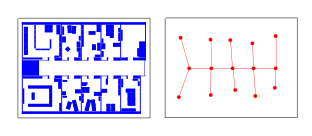
\includegraphics[width=0.7\linewidth]{Chapters/Chapter3/Figures/ogm_and_tm.png}
	\label{fig:ogm_and_tm}
	\caption[Μετρικός 2D χάρτης και αντίστοιχος τοπολογικός χάρτης σε μορφή γράφου.]{Μετρικός 2D χάρτης και αντίστοιχος τοπολογικός χάρτης σε μορφή γράφου \cite{probabilistic_robotics}.}
\end{figure}

\begin{figure}[!ht]
	\centering
	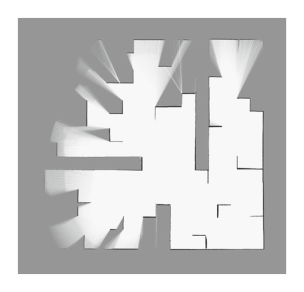
\includegraphics[width=0.4\linewidth]{Chapters/Chapter3/Figures/ogm.jpg}
	\label{fig:ogm}
	\caption[Χάρτης πλέγματος κατάληψης κελιού.]{Χάρτης πλέγματος κατάληψης κελιού \cite{crsm}.}
\end{figure}

\bigskip
Στην παρούσα διπλωματική εξετάστηκαν δύο αλγόριθμοι 2D SLAM, οι οποίοι χρησιμοποιούν αισθητήρες απόστασης και στην προκειμένη περίπτωση έναν {σαρωτή λέιζερ} και παράγουν χάρτες πλέγματος κατάληψης (Occupancy Grid Maps). Πρόκειται για τους αλγορίθμους CRSM-SLAM \cite{crsm} και GMapping \cite{gmapping}.

\bigskip
\subsubsection{CRSM-SLAM} \label{sssec:crsm_slam}
Ο αλγόριθμος CRSM-SLAM βασίζεται στην τεχνική της αντιστοίχισης σκαναρισμάτων απόστασης, που παρέχει ένας {σαρωτής λέιζερ}. Με βάση την τεχνική αυτή, η πόζα ενός ρομπότ και ο χάρτης, μπορούν να υπολογιστούν, χρησιμοποιώντας τον δισδιάστατο μετασχηματισμό μεταξύ διαδοχικών σκαναρισμάτων ενός σαρωτή λέιζερ. Ο αλγόριθμος CRSM-SLAM, πραγματοποιεί αντιστοίχιση σκαναραρισμάτων, σε σκαναρίσματα που έχουν υποστεί προεπεξεργασία, μέσω μίας μεθόδου επιλογής κρίσιμων, για την επιλογή, ακτίνων (ray selection method). Με αυτόν τον τρόπο, επιτυγχάνεται μείωση της πολυπλοκότητας και του χρόνου που απαιτείται για την διαδικασία αντιστοίχισης. Επίσης, πραγματοποιεί και αντιστοίχιση του τρέχοντος σκαναρίσματος, με τον ολικό χάρτη, που έχει κατασκευασθεί, με στόχο την μείωση των συσσωρευτικών σφαλμάτων.

\begin{figure}[!ht]
	\centering
	\includegraphics[width=0.4\linewidth]{Chapters/Chapter3/Figures/crsm_slam_diagram.png}
	\label{fig:crsm_slam_diagram.png}
	\caption[Διάγραμμα σταδίων του αλγορίθμου CRSM-SLAM.]{Διάγραμμα σταδίων του αλγορίθμου CRSM-SLAM \cite{crsm}.}
\end{figure}


\bigskip
Ο αλγόριθμος {CRSM-SLAM} αποτελεί μία αποδοτική και αξιόπιστη υλοποίηση, που μπορεί να χρησιμοποιηθεί σε υπολογιστικά συστήματα, με χαμηλή υπολογιστική ισχύ και απαιτεί μόνο έναν {σαρωτή λέιζερ} για την παροχή πληροφορίας για το περιβάλλον, για την χαρτογράφηση και τον εντοπισμό θέσης του ρομπότ. Παρόλα αυτά, προϋποθέτει ένα δομημένο περιβάλλον με αρκετά {κρίσιμα} χαρακτηριστικά (γωνίες, τελειώματα ή ασυνέχειες τοίχων κλπ.), έτσι ώστε να μπορεί να κάνει αξιόπιστη αντιστοίχιση των διαδοχικών σκαναρισμάτων. Επομένως, δεν είναι κατάλληλος για ανοιχτό περιβάλλον, ή μεγάλους ομοιόμορφους διαδρόμους, όπου δεν αρκεί η εμβέλεια του {σαρωτή λέιζερ}. 

\subsubsection{GMapping} \label{sssec:gmapping}
Ο αλγόριθμος {GMapping} αποτελεί έναν αλγόριθμο {SLAM}, που βασίζεται σε {Rao-Blackwellized φίλτρα σωματιδίων} για την παραγωγή {χαρτών πλέγματος κατάληψης}. Παράλληλα, χρησιμοποιεί, προσαρμοστικές τεχνικές για την μείωση του αριθμού των σωματιδίων, ενώ λαμβάνει υπόψιν την κίνηση του ρομπότ και τις πιο πρόσφατες μετρήσεις των αισθητήρων απόστασης, για την μείωση της αβεβαιότητας σχετικά με την πόζα του ρομπότ, κατά το στάδιο της πρόβλεψης.

\bigskip
Στην παρούσα διπλωματική, ο αλγόριθμος GMapping, χρησιμοποιήθηκε σε συνδυασμό με σκαναρίσματα από έναν σαρωτή λέιζερ και οδομετρία από ένα εκτεταμένο φίλτρο Kalman, που συνδυάζει πληροφορία οδομετρίας τροχών και πυξίδας για την παραγωγή μίας πιο εύρωστης εκτίμησης της κατάστασης του ρομπότ, σε αντίθεση με την χρήση απλής οδομετρίας. Το δεδομένο σύστημα, θα μπορούσε να επεκταθεί περαιτέρω με προσθήκη οπτικής οδομετρίας από κάμερα, αλλά και πληροφορία από αισθητήρα {GPS}. Η συμπερίληψη της οδομετρίας, κατά τον εντοπισμό θέσης, σε αντίθεση με τον αλγόριθμο {CRSM-SLAM}, καταστεί τον αλγόριθμο {GMapping} κατάλληλο και για εσωτερικούς και εξωτερικούς χώρους, αλλά με το μειονέκτημα των μεγαλύτερων απαιτήσεων σε πηγές πληροφορίας και μία υψηλή εξάρτηση από ένα εξωτερικό σύστημα εκτίμησης κατάστασης και της αντίστοιχης αξιοπιστίας αυτού. 

%----------------------------------------------------------------------------------------
%	SECTION 2: Autonomous Navigation
%----------------------------------------------------------------------------------------
\section{Αυτόνομη Πλοήγηση} \label{sec:autonomous_navigation}
Στις προηγούμενες ενότητες ασχοληθήκαμε με την κινηματική ανάλυση, την ρομποτική αντίληψη, την χαρτογράφηση και τον εντοπισμό θέσης, ικανότητες απαραίτητες για την αυτόνομη πλοήγηση σε άγνωστο περιβάλλον, δηλαδή την ικανότητα ενός ρομποτικού οχήματος να μεταβεί από μία αρχική θέση σε μία τελική, αυτόνομα, αποφεύγοντας, ταυτόχρονα εμπόδια και γενικότερα ανεπιθύμητες καταστάσεις.

\bigskip
Η αυτόνομη πλοήγηση ενός ρομποτικού οχήματος σχετίζεται άμεσα με την ευφυΐα ενός ρομπότ, όσον αφορά την λήψη αποφάσεων και την εκτέλεση στόχων που ορίζονται από λειτουργίες υψηλότερου επιπέδου, όπως για παράδειγμα η λειτουργία της \textit{επιλογής στόχων} (\textit{target selection}). Επομένως, η επάρκεια της ικανότητας αυτόνομης πλοήγησης ενός ρομπότ συνεπάγεται μία εύρωστη ευφυΐα κίνησης, ούτως ώστε με μερική γνώση του περιβάλλοντος και με δεδομένους στόχους να δρα αποδοτικά, αξιόπιστα και με ασφάλεια για την επίτευξη των στόχων αυτών.

\bigskip
Ένας πολύ σημαντικός όρος για τον τομέα της αυτόνομης πλοήγησης αποτελεί ο όρος της \textit{πληρότητας} (\textit{completeness}). Με βάση τον ορισμό της πληρότητας, ένα σύστημα αυτόνομης πλοήγησης είναι \textit{πλήρες}, εάν μπορεί να βρει λύση στο πρόβλημα επίτευξης ενός στόχου, εάν αυτή υπάρχει. Παρόλα αυτά, συνήθως, στις περισσότερες πρακτικές εφαρμογές, η πληρότητα του συστήματος θυσιάζεται για χάρη της υπολογιστικής πολυπλοκότητας. Επομένως, μας ενδιαφέρει η λύση ενός προβλήματος να μπορεί να βρεθεί σε πραγματικό χρόνο (real-time) και να καταναλώνει όσο το δυνατόν λιγότερους υπολογιστικούς πόρους.

\bigskip
Για την αντιμετώπιση του προβλήματος της αυτόνομης πλοήγησης, οι περισσότερες προσεγγίσεις προτείνουν κατανεμημένες αρχιτεκτονικές, που διασπούν το πρόβλημα σε επιμέρους υποπροβλήματα, προς αντιμετώπιση. Με αυτόν τον τρόπο επιτυγχάνεται δραστική μείωση της πολυπλοκότητας, παροχή δυνατότητας πιο αποδοτικής και απλουστευμένης υλοποίησης, ελέγχου και αποσφαλμάτωσης κάθε επιμέρους τμήματος, αλλά και δυνατότητα επαναχρησιμοποίησης τμημάτων σε άλλες προσεγγίσεις.

\bigskip
Η πιο δημοφιλής αρχιτεκτονική αυτόνομης πλοήγησης διασπά το πρόβλημα σε δύο επιμέρους υποπροβλήματα, προβλήματα αντίθετα, αλλά, ταυτόχρονα, συμπληρωματικά \cite{autonomous_mobile_robots}. Το πρώτο πρόβλημα προς επίλυση αποτελεί η \textit{κατασκευή μονοπατιού} (\textit{path planning}), η οποία, κατά το πλείστον, χρησιμοποιεί έναν χάρτη του περιβάλλοντος, τη θέση του ρομπότ και τη θέση του τρέχοντα στόχου, με σκοπό την κατασκευή ενός μονοπατιού που επιτρέπει στο ρομπότ την πλοήγηση προς τον στόχο, αποφεύγοντας στατικά εμπόδια. Το δεύτερο πρόβλημα προς επίλυση αποτελεί η \textit{αποφυγή εμποδίων}(\textit{obstacle avoidance}), η οποία χρησιμοποιεί τις πιο πρόσφατες μετρήσεις αισθητήρων ή και ένα τοπικό τμήμα του παραγομένου χάρτη, με στόχο την παραμόρφωση του κατασκευασμένου μονοπατιού για αποφυγή απρόσμενων εμποδίων και καταστάσεων, αλλά και την παραγωγή εφικτών κινηματικά και δυναμικά τροχιών, από το ρομπότ. Επομένως, η κατασκευή μονοπατιού σχετίζεται με μακροπρόθεσμο σχεδιασμό για την επίτευξη του δοσμένου στόχου, ενώ η αποφυγή εμποδίων σχετίζεται με την βραχυπρόθεσμη λήψη αποφάσεων για την ασφαλή πλοήγηση προς τον δοσμένο στόχο, συνδυάζοντας σχεδιασμό και εκτέλεση, βάσει της πιο πρόσφατης αντίληψης για το περιβάλλον.

\bigskip
Στην παρούσα διπλωματική εξετάζονται δύο αρχιτεκτονικές συστήματος αυτόνομης πλοήγησης. Η πρώτη αρχιτεκτονική επεκτείνει την προσέγγιση, που αναφέρθηκε παραπάνω, διασπώντας τη λειτουργία της αποφυγής εμποδίων σε τρία επιμέρους στάδια. Το σύνολο των σταδίων αυτών, αποτελείται από ένα στάδιο παραμόρφωσης μονοπατιού για απομάκρυνση από εμπόδια, στατικά ή δυναμικά, ένα στάδιο μετατροπής του παραμορφωμένου μονοπατιού σε ένα νέο κινηματικά εφικτό μονοπάτι και ένα τελευταίο στάδιο που είναι υπεύθυνο για την διάσχιση του μονοπατιού, μέσω κινηματικά εφικτών εντολών στο χώρο \textit{ταχύτητας-στρέψης} ($v$, $\delta_f$, $\delta_r$). Αντίθετα, η δεύτερη αρχιτεκτονική που εξετάζεται χρησιμοποιεί έναν αλγόριθμο κατασκευής κινηματικά εφικτών μονοπατιών με δυναμική ανακατασκευή (dynamic replanning), σε περίπτωση δυναμικών εμποδίων ή γενικά απρόσμενων καταστάσεων, σε συνδυασμό με έναν αλγόριθμο διάσχισης μονοπατιού, αντίστοιχο της πρώτης προσέγγισης.

\bigskip
Η κατασκευή μονοπατιών και η αποφυγή εμποδίων πραγματοποιούνται σε μία αναπαράσταση του περιβάλλοντος, μέσω χαρτών κόστους. Οι \textit{χάρτες κόστους} (\textit{costmaps}) είναι μία δομή αναπαράστασης του περιβάλλοντος που συντίθεται από ένα σύνολο \textit{επιπέδων} (\textit{layers}). Στην προκειμένη περίπτωση, χρησιμοποιούνται τρία επίπεδα, το \textit{στατικό επίπεδο} \textit{static layer} που αναπαριστά τα σχετικά αμετάβλητα τμήματα του χάρτη όπως αυτά παράγονται από έναν αλγόριθμο SLAM, το \textit{επίπεδο εμποδίων} (\textit{obstacle layer}) που αποτελεί μία 2D αναπαράσταση των εμποδίων του περιβάλλοντος, όπου τα κελιά των εμποδίων περιγράφονται από ένα \textit{απαγορευτικό κόστος} (\textit{lethal cost}) που δηλώνει μη προσπελασιμότητα και το \textit{επίπεδο διαστολής} (\textit{inflation layer}) που διαδίδει τα απαγορευτικά κόστη ακτινικά με αποσβενόμενο κόστος κατά μία απόσταση που προσδιορίζεται από τον χρήστη κάθετα από τα εμπόδια. Στα κελιά που βρίσκονται σε απόσταση από τα εμπόδια, μικρότερη της ακτίνας εγγεγραμμένου, στο ρομπότ, κύκλου, ανατίθεται ένα υψηλό κόστος, ενώ στα επόμενα το κόστος υπολογίζεται από μία εκθετικά φθίνουσα συνάρτηση, τέτοια ώστε το κόστος μηδενίζεται σε απόσταση ίση με την απόσταση που ορίστηκε από τον χρήστη. Με αυτόν τον τρόπο, το ρομπότ μπορεί να αντιμετωπίζεται σαν σημείο που κινείται στον ελεύθερο χώρο, όπου ως ελεύθερος χώρος ορίζεται το σύνολο των κελιών του χάρτη κόστους με μηδενικό κόστος, ή αρκετά χαμηλό κόστος που προσδιορίζεται από τον χρήστη.

\bigskip
Στην συνέχεια, θα παρουσιαστούν τα αντικείμενα της κατασκευής μονοπατιών, της αποφυγής εμποδίων και της διάσχισης μονοπατιού όπως επίσης και η σχετική βιβλιογραφία, αλλά και οι τελικοί αλγόριθμοι που χρησιμοποιήθηκαν στο σύστημα αυτόνομης πλοήγησης της ρομποτικής πλατφόρμας Monstertruck.

\subsection{Κατασκευή Μονοπατιού} \label{ssec:path_planning}
%-------------------------------%
Το αντικείμενο της κατασκευής μονοπατιών ξεκίνησε με τους βιομηχανικούς ρομποτικούς βραχίονες για την αυτοματοποίηση γραμμών παραγωγής σε εργοστάσια, αλλά από τότε έχει περιλάβει κάθε είδους ρομποτική εφαρμογή, όπως και η κατασκευή μονοπατιών για πλοήγηση ρομπότ στο επίπεδο (2D path planning) ή στο χώρο (3D path planning), πρόβλημα που αποτελεί αρκετά απλούστερο από αυτό των ρομποτικών βραχιόνων, λόγω λιγότερων βαθμών ελευθερίας και άρα λιγότερες διαστάσεις.

\bigskip
Πριν προχωρήσουμε στην κατασκευή μονοπατιών, αυτή καθ' αυτή, θα πρέπει πρώτα να περιγράψουμε την αναπαράσταση του χώρου στον οποίο πραγματοποιείται η εργασία αυτή. Η αναπαράσταση αυτή, ονομάζεται \textit{χώρος καταστάσεων} (\textit{configuration space}) $C$ και έχει τόσες διαστάσεις όσες και οι βαθμοί ελευθερίας (DOF) του ρομπότ. Στην προκειμένη περίπτωση, εφόσον έχουμε ένα ρομποτικό όχημα που κινείται στο επίπεδο, μιλάμε για τρεις βαθμούς ελεθερίας (3-DOF), όσον αφορά τις καρτεσιανές συντεταγμένες θέσης $(x, y)$ και τον προσανατολισμό $\theta$ του ρομπότ. Ο χώρος αυτός αποτελείται από όλες τις δυνατές καταστάσεις (configurations) $(x, y, \theta)$ που μπορεί να βρεθεί το ρομπότ στον χώρο. Στις περισσότερες περιπτώσεις ένας χώρος δεν είναι πλήρως ελεύθερος, αλλά περιλαμβάνει εμπόδια. Επομένως, ως ελεύθερος χώρος $C_{free}$ ορίζεται ο χώρος καταστάσεων μείον τον υποχώρο των εμποδίων $C_O$, δηλαδή $C_{free} = C - C_O$ και αποτελεί το υποσύνολο του χώρου, στο οποίο, το ρομπότ μπορεί να κινηθεί χωρίς να υποστεί συγκρούσεις.

\bigskip
Ο παραπάνω χώρος καταστάσεων $C$ περιορίζεται περαιτέρω, αν αναλογιστεί κανείς, ότι τα περισσότερα ρομπότ χρησιμοποιούν κινηματικά μοντέλα, όπως Differential-Drive, Skid-Steer- Drive, Ackermann ή Four-Wheel Steering, τα οποία παρουσιάζουν \textit{μη ολονομικούς περιορισμούς} (\textit{nonholonomic constraints}) που περιορίζουν τον χώρο ταχυτήτων $(\dot x, \dot y, \dot \theta)$, σε αντίθεση με \textit{ολονομικά} (\textit{holonomic}) \textit{πανκατευθυντικά} (\textit{omnidirectional}) ρομπότ. Παρόλα αυτά, η συνήθης προσέγγιση έγκειται στην αγνόηση της μη ολονομικότητας για την κατασκευή μονοπατιών, καθώς τα πιο συνήθη ρομποτικά κινηματικά μοντέλα Differential-Drive και Skid-Steer-Drive, θεωρούνται ως ψευδο-ολονομικά, καθώς διαθέτουν δυνατότητα επιτόπου στροφής (0-point turn) και μπορούν να ακολουθήσουν ολονομικά μονοπάτια, ενώ ίδια προσέγγιση ακολουθείται και για ρομπότ με Ackermann ή Four-Wheel Steering, αλλά στην συγκεκριμένη περίπτωση, το πρόβλημα της διάσχισης του μονοπατιού λύνεται σε επόμενο στάδιο. Επίσης, στις περισσότερες προσεγγίσεις, για την διευκόλυνση του προβλήματος της κατασκευής μονοπατιών λαμβάνεται η παραδοχή ότι το ρομπότ είναι ένα κινούμενο σημείο στο 2D χώρο $(x, y)$, ενώ αντί για τα πραγματικά εμπόδια, λαμβάνεται μία διασταλμένη εκδοχή αυτών, κατά την ακτίνα ενός κύκλου, στον οποίο εγγράφεται το ίχνος/αποτύπωμα του ρομπότ. Τέλος, όπως είναι φυσικό, έχουν μελετηθεί και αναπτυχθεί και διαφορετικές προσεγγίσεις που λαμβάνουν υπόψιν κινηματικούς και δυναμικούς περιορισμούς στο στάδιο της κατασκευή μονοπατιού, κατάλληλοι για μη ολονομικά οχήματα. Παρακάτω, θα εξεταστούν και οι δύο περιπτώσεις.

\begin{figure}[!ht]
	\centering
	\includegraphics[width = 0.7\linewidth]{Chapters/Chapter3/Figures/point_robot_and_inflated_obstacles.png}
	\caption[Αναπαράσταση ρομπότ ως σημείο και διαστολή εμποδίων, βάσει της ακτίνας του ρομπότ. ]{Αναπαράσταση ρομπότ ως σημείο και διαστολή εμποδίων, βάσει της ακτίνας του ρομπότ \cite{principles_of_robot_motion}.}
	\label{fig:point_robot_and_inflated_obstacles}
\end{figure}

\bigskip
Όπως αναφέρθηκε παραπάνω, η κατασκευή μονοπατιών λαμβάνει χώρα πάνω σε έναν χάρτη κόστους, ο οποίος παράγεται από τον συνολικό τρέχοντα χάρτη πλέγματος κατάληψης, που έχει παραχθεί από έναν αλγόριθμο SLAM και ονομάζεται \textit{ολικός χάρτης κόστους} (\textit{global costmap}). Ο ολικός χάρτης κόστους, έπειτα, αντιμετωπίζεται ως γράφος και επομένως, η κατασκευή μονοπατιού μετασχηματίζεται σε αναζήτηση μονοπατιού σε γράφο.

\bigskip 
\subsubsection{Αναζήτηση Μονοπατιού σε Γράφο} \label{sssec:graph_search}
Ως \textit{γράφος} $G$ ορίζεται μία συλλογή από \textit{κόμβους} $V$ και \textit{ακμές} $E$. Στην κατασκευή μονοπατιών, ένας κόμβος $V$ αναπαριστά μία θέση στον χώρο, ενώ μία ακμή $E$ αναπαριστά την σύνδεση μεταξύ δύο γειτονικών κόμβων, όπου δύο κόμβοι ορίζεται ως \textit{γειτονικοί} εάν είναι προσπελάσιμοι ο ένας από τον άλλο. Μία ακμή είναι \textit{κατευθυνόμενη} εάν επιτρέπει την μονόδρομη μετάβαση από έναν κόμβο $V_i$ σε έναν άλλο $V_j$ ($E_{ij}$ ή $E_{ji}$) ή μη κατευθυνόμενη εάν επιτρέπει αμφίδρομη μετάβαση ($E_{ij}$ και $E_{ij}$). Επίσης, σε κάθε ακμή $E_{ij}$ ανατίθεται μία τιμή που αναπαριστά το κόστος μετάβασης από τον κόμβο $V_i$ προς έναν γειτονικό κόμβο $V_j$ και ονομάζεται βάρος $w_{ij}$ της ακμής.

\begin{figure}[!ht]
	\centering
	\includegraphics[width=0.6\linewidth]{Chapters/Chapter3/Figures/directed_and_non_graph.png}
	\caption[Κατευθυνόμενος (αριστερά) και μη κατευθυνόμενος (δεξιά) γράφος.]{Κατευθυνόμενος (αριστερά) και μη κατευθυνόμενος (δεξιά) γράφος \cite{principles_of_robot_motion}.}
	\label{fig:directed_and_non_graph}
\end{figure}

\bigskip
Ως μονοπάτι στον γράφο ορίζεται μία ακολουθία κόμβων $V_i$, τέτοια ώστε, για κάθε $V_i$, $V_{i+1}$ υπάρχει μία ακμή $E_{i\;i+1}$ που ενώνει τους κόμβους $V_i$, $V_{i+1}$. Αν υπάρχει ακμή $E_ij$ για κάθε συνδυασμό κόμβων $V_i$, $V_j$, τότε ο γράφος είναι \textit{συδεδεμένος}.

\bigskip 
Τα δέντρα αποτελούν μία υποπερίπτωση των γράφων και ορίζονται ως συνδεδεμένοι, καυτευθυντικοί άκυκλοι γράφοι, όπου ένας γράφος θεωρείται \textit{άκυκλος} εάν δεν περιέχει κυκλικά μονοπάτια, δηλαδή μονοπάτια που αποτελούνται από μία ακολουθία $n$ κόμβων, όπου ο πρώτος κόμβος $V_1$ ταυτίζεται με τον τελευταίο $V_n$. Τα δέντρα έχουν έναν αρχικό κόμβο, που ονομάζεται ρίζα και συνδέεται μόνο με εξερχόμενες ακμές (outgoing) και όχι με εισερχόμενες (incoming). Στα δέντρα, επίσης χρησιμοποιείται μία \textit{τοπολογία πατέρα - παιδιού}, όπου κάθε κόμβος έχει πατέρα (εκτός τη ρίζα) και μπορεί να έχει από μηδέν ή περισσότερα παιδιά. Εάν ένας κόμβος δεν περιλαμβάνει παιδιά, αυτό υποδηλώνει ότι είναι τερματικός κόμβος και ονομάζεται \textit{φύλλο} (\textit{leaf}) του δέντρου.

\begin{figure}[!ht]
	\centering
	\includegraphics[width=0.3\linewidth]{Chapters/Chapter3/Figures/tree.png}
	\caption[Δέντρο: συνδεδεμένος, καυτευθυνόμενος και άκυκλος γράφος.]{Δέντρο: συνδεδεμένος, καυτευθυνόμενος και άκυκλος γράφος \cite{principles_of_robot_motion}.}
	\label{fig:tree}
\end{figure}


\bigskip
Η αναζήτηση μονοπατιού από έναν αρχικό κόμβο προς ένα κόμβο - στόχο σε ένα δέντρο, πραγματοποιείται με μεθόδους αναζήτησης μονοπατιού. Υπάρχουν δύο βασικές προσεγγίσεις που διακρίνονται, η \textit{αναζήτηση κατά βάθος} (\textit{depth-first search}) και η \textit{αναζήτηση κατά πλάτος}(\textit{breadth-first search}). Η αναζήτηση κατά βάθος ξεκινά από την ρίζα του δέντρου, επιλέγει ένα παιδί της ρίζας, έπειτα ένα παιδί του παιδιού της ρίζας και ούτω καθεξής, μέχρις ότου να βρεθεί σε φύλλο ή στον στόχο. Εάν βρεθεί σε φύλλο, τότε ανεβαίνει ένα επίπεδο πάνω και προχωράει στο επόμενο παιδί. Η διαδικασία αυτή επαναλαμβάνεται, μέχρις ότου βρεθεί ο στόχο ή καλυφθούν όλοι οι κόμβοι του δέντρου. Αντίθετα, η  αναζήτηση κατά πλάτος, λειτουργεί με την πεποίθηση ότι ο στόχος βρίσκεται κοντά στον αρχικό κόμβο - ρίζα. Έτσι, λοιπόν, ξεκινάει από την ρίζα, επισκέπτεται όλα τα παιδιά της ρίζας και έπειτα όλα τα εγγόνια (παιδιά των παιδιών) της ρίζας και ούτω καθεξής, μέχρις ότου επισκεφθεί τον στόχο, ή μέχρι να καλύψει όλους τους κόμβους του δέντρου.

\begin{figure}[!ht]
	\centering
	\includegraphics[width=0.6\linewidth]{Chapters/Chapter3/Figures/tree_search_methods.png}
	\caption[Μέθοδοι αναζήτησης κατά βάθος (αριστερά) και κατά πλάτος (δεξιά) σε δέντρο.]{Μέθοδοι αναζήτησης κατά βάθος (αριστερά) και κατά πλάτος (δεξιά) σε δέντρο \cite{principles_of_robot_motion}.}
	\label{fig:tree_search_methods}
\end{figure}

\bigskip
Σε ρομποτικές εφαρμογές, συνήθως χρησιμοποιείται ένα \textit{πλέγμα} (\textit{grid}), για την αναπαράσταση του χώρου. Η δομή του πλέγματος, μπορεί να θεωρηθεί ως γράφος, εάν λάβουμε ως κόμβους του γράφου, τα pixels του πλέγματος και ως ακμές τις ενώσεις γειτονικών κελιών. Η γειτονικότητα των κελιών, συνήθως ορίζεται με βάση τον ορισμό της συνδετικότητας του γράφου, όπου επιλέγεται συνήθως συνδετικότητα τεσσάρων σημείων ή οκτώ σημείων, όπως παρουσιάζεται στο σχήμα \ref{fig:graph_connectivity}.

\begin{figure}[!ht]
	\centering
	\includegraphics[width=0.5\linewidth]{Chapters/Chapter3/Figures/graph_connectivity.png}
	\caption[Πλέγμα και γράφοι συνδετικότητας τεσσάρων και οκτώ σημείων (από αριστερά προς τα δεξιά).]{Πλέγμα και γράφοι συνδετικότητας τεσσάρων και οκτώ σημείων (από αριστερά προς τα δεξιά) \cite{principles_of_robot_motion}.}
	\label{fig:graph_connectivity}
\end{figure}

\bigskip
Οι γράφοι πλέγματος, όπως είναι προφανές, δεν αποτελούν δέντρα. Παρόλα αυτά, με κάποιες παραδοχές, γίνεται, δυνατή η χρήση των προαναφερθέντων μεθόδων αναζήτησης κατά βάθος και κατά πλάτος. Συγκεκριμένα, η αναζήτηση κατά βάθος ξεκινάει από τον αρχικό κόμβο, επιλέγει ένα παιδί - κόμβο και μετέπειτα παιδιά - κόμβους με αυξανόμενη απόσταση από τον αρχικό κόμβο, μέχρις ότου βρεθεί σε κόμβο χωρίς παιδιά ή σε κόμβο που έχει ήδη επισκεφθεί. Αντίστοιχα, η αναζήτηση κατά πλάτος επισκέπτεται πρώτα τα κόμβους που ισαπέχουν από τον αρχικό κόμβο και έπειτα μεταβαίνει σε επόμενα επίπεδα κόμβων. Τέλος, υπάρχει και η περίπτωση των άπληστων μεθόδων αναζήτησης γράφων (greedy-search methods) που επεκτείνονται σε κόμβους που βρίσκονται κοντινότερα στον κόμβο, που έχει οριστεί ως στόχος. 

\subsubsection{Αλγόριθμοι Dijkstra και A*} \label{sssec:dijkstra_astar}
Οι πιο γνωστοί και δημοφιλείς αλγόριθμοι αναζήτησης μονοπατιού σε γράφο είναι οι αλγόριθμοι Dijkstra και A*. Ο αλγόριθμος Dijkstra αναπτύχθηκε από τον Edsger W. Dijkstra, το 1956, με στόχο την αναζήτηση του συντομότερου μονοπατιού διάσχισης μεταξύ δύο κόμβων σε έναν γράφο, βάσει αναζήτησης κατά πλάτος. Ο αλγόριθμος Α* αποτελεί μία γενίκευση του αλγορίθμου Dijkstra, που αναπτύχθηκε το 1968 από τους Peter Hart, Nils Nilsson και Bertram Raphael και βασίζεται στην χρήση \textit{ευρετικών} (\textit{heuristics}) μεθόδων για την κατεύθυνση του αναζήτησης, με στόχο την βελτιστοποίηση της όλης διαδικασίας αναζήτησης, όσον αφορά την ελαχιστοποίηση του αριθμού των επισκεπτόμενων κόμβων, την ελαχιστοποίηση του χρόνου εκτέλεσης κλπ.

\bigskip
Το μειονέκτημα των μεθόδων αναζήτησης κατά βάθος και κατά πλάτος, έγκειται στο γεγονός ότι δεν χρησιμοποιούν πληροφορία σχετικά με την θέση του κόμβου, που έχει οριστεί ως στόχος, για να κατευθύνουν την αναζήτηση. Το πρόβλημα αυτό λύνεται, από τον αλγόριθμο A* ο οποίος απαιτεί τον ορισμό μίας ευρετικής μεθόδου για την εκτίμηση του κόστους για την μετάβαση από έναν κόμβο στον δεδομένο στόχο. Η ευρετική αυτή μέθοδος χρησιμοποιείται κατά την επιλογή του νέου κόμβου, βάσει της απόστασης του από τον στόχο. Ο νέος στόχος, επομένως, πρέπει να εκφράζει την υψηλότερη πιθανότητα προσέγγισης του στόχου, με βάση τοπική πληροφορία. Η μέθοδος αυτή, παρόλα αυτά, δεν προσφέρει καμία εγγύηση για την σύγκλιση στο ολικώς βέλτιστο μονοπάτι.

\bigskip
Η απόδοση του αλγορίθμου A* βασίζεται στην επιλογή μίας καλής ευρετικής μεθόδου και επομένως, καθορίζει την πιθανότητα εύρεσης του βέλτιστου μονοπατιού. Μία ευρετική μέθοδος, θεωρείται καλή εάν είναι αισιόδοξη, δηλαδή εάν επιστρέφει κόστος, μικρότερο ή ίσο με το μήκος του βέλτιστου μονοπατιού για την μετάβαση από τον τρέχον κόμβο στον στόχο. Για παράδειγμα, μία αισιόδοξη ευρετική μέθοδος, που χρησιμοποιείται συχνά, είναι η ευκλείδια απόσταση ή απόσταση Manhattan μεταξύ του τρέχοντος κόμβου και του στόχου.

\bigskip
Αν ορίσουμε ως $h(n)$ την ευρετική συνάρτηση και $g(n)$ την συνάρτηση κόστους μετάβασης από τον αρχικό στον τρέχοντα κόμβο, τότε η συνάρτηση $f(n)$ που δηλώνει την εκτίμηση του κόστους μετάβασης από τον αρχικό κόμβο στον τελικό στόχο, μέσω του κόμβου $n$ ορίζεται ως

\begin{equation}\label{eq:astar_cost}
	f(n) = g(n) + h(n)
\end{equation}

\bigskip
Εδώ αξίζει να αναφερθεί, ότι αν λάβουμε $h(n)=0$, η σχέση (\ref{eq:astar_cost}) περιγράφει το κόστος επιλογής νέου κόμβου του αλγορίθμου Dijkstra, ενώ αν λάβουμε $g(n)=0$, τότε παίρνουμε την αντίστοιχη επιλογή νέου κόμβου του άπληστου αλγορίθμου αναζήτησης.

\begin{figure}[!ht]
	\centering
	\subfloat[Dijkstra]{
		\includegraphics[width=0.3\linewidth]{Chapters/Chapter3/Figures/dijkstra.jpg}}
	\subfloat[Greedy]{
		\includegraphics[width=0.3\linewidth]{Chapters/Chapter3/Figures/greedy.jpg}}
	\subfloat[A*]{
		\includegraphics[width=0.3\linewidth]{Chapters/Chapter3/Figures/astar.jpg}}
	\caption[Σύγκριση αλγορίθμων αναζήτησης μονοπατιού σε γράφο πλέγματος Dijkstra, Greedy και A*.]{Σύγκριση αλγορίθμων αναζήτησης μονοπατιού σε γράφο πλέγματος με Dijkstra, Greedy και A* \cite{etsardou_phd}.}
	\label{fig:astar_and_dijkstra_comparison}
\end{figure}

% Τέλος, παρακάτω παρουσιάζεται ο ψευδοκώδικας του αλγορίθμου Α*.
%\begin{algorithm}
%	\label{alg:astar}
%	\caption{Αλγόριθμος A*}
%	\textbf{Input:} Graph\\
%	\textbf{Output:} Path between start and goal nodes
%	\begin{algorithmic}[1]
%		\Do
%			\State Pick $n_{best}$ from $O$ such that $f(n_{best}) \leq f(n),\, \forall  n \in O$.
%			\State Remove $n_{best}$ from $O$ and add to $C$.
%			\If{ $n_{best} = q_{goal}$}
%				 \State Return $O$
%			\EndIf
%			\State Expand $n_best$: $\forall x \in Star(n_{best})$ that are not in $C$.
%			\If{ $x \notin O$}
%				\State Add $x$ to $O$.
%			\Else{ \textbf{if} $g(n_{best}) + c(n_{best},x) < g(x)$\,\textbf{then}}
%				\State Update $x'$s backpointer to point to $n_{best}$.
%			\EndIf
%		\doWhile{ $O$ is not empty}
%	\end{algorithmic}
%\end{algorithm}
%
%\bigskip\noindent
%όπου
%\begin{description}
%	\item[Star(n):] το σετ των κόμβων που είναι γειτονικοί στον κόμβο $n$
%	\item[c(n_1, n_2):] μήκος ακμής μεταξύ κόμβων $n_1$ και $n_2$
%	\item[g(n):] μήκος μονοπατιού από τον κόμβο n μέχρι τον αρχικό κόμβο $q_{start}$
%	\item[h(n):] ευρετική συνάρτηση κόστους που επιστρέφει την εκτίμηση κόστους κοντινότερου μονοπατιού από τον κόμβο $n$ μέχρι τον αρχικό κόμβο $q_{start}$
%	\item[f(n)=g(n)+h(n):] εκτίμηση κόστους κοντινότερου μονοπατιού από τον αρχικό κόμβο $q_{start}$ μέχρι τον τελικό $q_{goal}$, μέσω του κόμβου $n$.
%\end{description}

\bigskip
Οι αλγόριθμοι Dijkstra και A* που εφαρμόζονται στον χώρο καταστάσεων, όπως παρουσιάστηκαν παραπάνω και με βάση τις παραδοχές που αναφέρθηκαν για την γεωμετρία και κινητικότητα του ρομπότ, αγνοούν πλήρως κινηματικούς και δυναμικούς περιορισμούς, που μπορεί να παρουσιάζει αυτό. Επίσης, αποτελούν μεθόδους ακατάλληλες για δυναμικά περιβάλλοντα, όπου ένα μονοπάτι, μπορεί να καταστεί μη προσπελάσιμο, με βάση τις πιο σύγχρονες πληροφορίες σχετικά με το περιβάλλον.



\subsubsection{Αλγόριθμος SBPL Lattice Planner} \label{sssec:sbpl}
Οι Maxim Likhachev και Dave Ferguson \cite{sbpl} προτείνουν έναν αλγόριθμο κατασκευής δυναμικά εφικτών μονοπατιών, μεγάλου μήκους για αυτόνομα οχήματα που κινούνται με υψηλές ταχύτητες (~25kph), ο οποίος χρησιμοποιήθηκε στον διαγωνισμό DARPA Urban Challenge, με πολύ θετικά αποτελέσματα. Ο αλγόριθμος, αυτός, βασίζεται σε μία \textit{χρονικά άμεση} και \textit{σταδιακή} αναζήτηση (\textit{anytime $\&$ incremental search}) σε ένα \textit{πολλαπλής-ανάλυσης δικτύωμα δυναμικά εφικτών καταστάσεων} (\textit{multi-resolution dynamically feasible lattice state space}).

\bigskip
Το \textit{δικτύωμα καταστάσεων} (\textit{state lattice}) ορίζεται ως μία διακριτοποίηση του χώρου καταστάσεων σε ένα σετ καταστάσεων και τις αντίστοιχες συνδέσεις μεταξύ αυτών, όπου μία σύνδεση μεταξύ δύο καταστάσεων, δηλώνει ένα εφικτό μονοπάτι. Επομένως, το πρόβλημα κατασκευής μονοπατιών μετασχηματίζεται και πάλι σε αναζήτηση σε γράφο. Σε αντίθεση με γράφους με συνδετικότητα τεσσάρων ή οκτώ σημείων, ο ορισμός της συνδετικότητας καταστάσεων στα δικτυωμάτα καταστάσεων εγγυάται ότι όποια λύση βρεθεί θα είναι κινηματικά και δυναμικά εφικτή, γεγονός που καθιστά τον εν λόγω αλγόριθμο κατάλληλο για μη ολονομικά οχήματα.

\bigskip
Στην προκειμένη περίπτωση για την αναπαράσταση μίας κατάστασης χρησιμοποιείται το διάνυσμα τεσσάρων μεταβλητών $s=(x, y, \theta, v)$, όπου $(x, y)$ είναι οι καρτεσιανές συντεταγμένες, $\theta$ ο προσανατολισμός και $v$ η ταχύτητα για την δεδομένη κατάσταση. Οι συντεταγμένες και ο προσανατολισμός είναι βασικοί για τον έλεγχο της εγκυρότητας μίας πόζας, δηλαδή κατά πόσο είναι εφικτή, ενώ η ταχύτητα που μπορεί να πάρει μόνο μέγιστη κατά απόλυτο τιμή, χρησιμοποιείται για να λαμβάνεται υπόψιν ο χρόνος που απαιτείται για την αντιστροφή της ταχύτητας, σε περιπτώσεις ελιγμών.

\bigskip
Για την κατασκευή των δικτυωμάτων καταστάσεων λαμβάνονται υπόψιν δύο βασικά σημεία. Πρώτον η  διακριτοποίηση / δειγματοληψία του χώρου καταστάσεων για την αναπαράσταση των καταστάσεων στο δικτύωμα και δεύτερον η κατασκευή ενός \textit{χώρου κινήσεων}(\textit{action space / control set}) που ορίζει τις δυναμικά εφικτές συνδέσεις μεταξύ δυο καταστάσεων. Ο χώρος κινήσεων θα πρέπει να είναι αρκετά πλήρης, ώστε να καθιστά δυνατή την κατασκευή όλων των δυνατών μονοπατιών στο δικτύωμα καταστάσεων, μέσω συνδυασμού ακολουθιών των βασικών δυνατών κινήσεων (motion primitives).

\bigskip
Για την μείωση του κόστους ελέγχου όλων των συνδυασμών των δυνατών κινήσεων για την κατασκευή ενός μονοπατιού μεταξύ δύο καταστάσεων, ο αλγόριθμος χρησιμοποιεί μία προσέγγιση πολλαπλής ανάλυσης, με βάση την οποία χρησιμοποιείται ένας χώρος ελέγχου υψηλής ανάλυσης για περιοχές κοντά στην αρχική και τελική κατάσταση και ένας χώρος ελέγχου χαμηλής ανάλυσης για το ενδιάμεσο τμήμα.

\bigskip
Η αναζήτηση στο δικτύωμα καταστάσεων πραγματοποιείται με βάση τις δυνατές κινήσεις και τα κόστη αυτών. Η πιο δημοφιλής μέθοδος αναζήτησης είναι ο αλγόριθμος A*, ο οποίος είναι αρκετά αποδοτικός και στοχεύει στην εύρεση του βέλτιστου μονοπατιού μεταξύ δύο καταστάσεων. Παρόλα αυτά λόγω του μεγέθους του προβλήματος που καλείται να λύσει, μπορεί να παραβιάζει χρονικούς περιορισμούς και άρα καθίσταται ανεπαρκής. Μία λύση στο πρόβλημα αυτό προσφέρουν παραλλαγές του αλγορίθμου A* που βασίζονται στην προσέγγιση της χρονικής αμεσότητας (Anytime A* variants), όπως ο αλγόριθμος ARA* (Anytime Repairing A*). Οι αλγόριθμοι, που ανήκουν σ' αυτήν την κατηγορία στοχεύουν στην εύρεση μίας αρχικής άκρως μη βέλτιστης λύσης, αλλά σε πολύ μικρό χρόνο, ενώ έπειτα, ασχολούνται με την συνεχή βελτίωση της λύσης αυτής, όσο επιτρέπεται από τους χρονικούς περιορισμούς.

\begin{figure}[!ht]
	\centering
	\includegraphics[width=\linewidth]{Chapters/Chapter3/Figures/arastar.png}
	\caption[Αναζήτηση σε γράφο πλέγματος με Α* (αριστερά) και ARA* (δεξιά) για μειούμενο παράγοντα διαστολής $\epsilon$.]{Αναζήτηση σε γράφο πλέγματος με Α* (αριστερά) και ARA* (δεξιά) για φθίνοντα παράγοντα διαστολής $\epsilon$ \cite{arastar}.}
	\label{fig:arastar}
\end{figure}

\bigskip
Ο αλγόριθμος Α* και οι παραλλαγές του δουλεύουν αποτελεσματικότερα, όταν το περιβάλλον εργασίας είναι γνωστό από πριν και δεν μεταβάλλεται, κάτι αρκετά απίθανο στις περισσότερες ρομποτικές εφαρμογές. Ένα ρομπότ, δέχεται συνεχώς δεδομένα από τους αισθητήρες του μπορεί να μεταβάλλουν την αντίληψη του για το περιβάλλον και άρα μία λύση να καθίσταται μη εφικτή. Επίσης, τα περισσότερα περιβάλλοντα είναι \textit{δυναμικά}, δηλαδή περιλαμβάνουν κινούμενα αντικείμενα, όπως άλλα ρομπότ, οχήματα, ανθρώπους κα., στα οποία θα πρέπει να μπορεί να αντιδράσει το ρομπότ για να αποφύγει πιθανές συγκρούσεις. Το πρόβλημα αυτό θα μπορούσε να λυθεί χρησιμοποιώντας συνεχής ανανέωση του μονοπατιού, λύση που αποτελεί ιδιαίτερα κοστοβόρα και μπορεί να μην είναι χρονικά εφικτή. Επομένως, απαιτείται μία λύση που να στοχεύει στην \textit{επιδιόρθωση} τμημάτων της υπάρχουσας λύσης και όχι στην αντικατάστασης της από νέα, όπως για παράδειγμα ο αλγόριθμος D* και οι παραλλαγές του.

\bigskip
Ο αλγόριθμος αναζήτησης που προτείνουν οι Likhachev και Ferguson, είναι ο αλγόριθμος AD* (Anytime Dynamic A*). Ο αλγόριθμος AD* συνδυάζει τα θετικά και των δύο παραπάνω κατηγοριών, παραλλαγών Anytime A* και D* αλγορίθμων. Συγκεκριμένα, πραγματοποιεί μη βέλτιστες αναζητήσεις A*, μέσω διαστολής του κόστους λύσης κατά έναν μειούμενο παράγοντα $\epsilon > 1$, χρησιμοποιώντας παράλληλα πληροφορία από την προηγούμενη αναζήτηση. Επίσης, δανείζεται ιδέες από τον αλγόριθμο D* και τις παραλλαγές του, βάσει των οποίων, χρησιμοποιεί καινούργιες πληροφορίες, μόνο για τμήματα του χώρου αναζήτησης, που αφορούν την τρέχουσα κατάσταση και αναζήτηση. Αυτό επιτυγχάνεται με ανανέωση του μονοπατιού, μέσω αναζήτησης από την τελική κατάσταση (στόχος) προς τα πίσω μέχρι την τρέχουσα κατάσταση του ρομπότ.

\bigskip
Η απόδοση του αλγορίθμου AD*, όπως και του αλγοριμου Α*, βασίζεται απόλυτα στην επιλογή μίας αποδοτικής ευρετικής συνάρτησης $h(n)$ για την κατεύθυνση της αναζήτησης, η οποία μπορεί να μειώσει της απαιτήσεις της αναζήτησης σε χρόνο και μνήμη κατά τουλάχιστον μία τάξη μεγέθους. Μία γενική αισιόδοξη ευρετική συνάρτηση που μπορεί να χρησιμοποιηθεί αποτελεί η βέλτιστη λύση σε περιβάλλον χωρίς εμπόδια, που μπορεί να υπολογιστεί \textit{offline} και να αποθηκευθεί σε έναν ευρετικό πίνακα για ένα δεδομένο περιβάλλον. Παρόλα αυτά, η λύση αυτή δεν είναι πρακτική για διάφορα περιβάλλοντα. Αντίθετα, προτιμότερη είναι η \textit{online} λύση ενός απλοποιημένου προβλήματος αναζήτησης και η χρήση του αποτελέσματος για την κατεύθυνση του πιο σύνθετου προβλήματος αναζήτησης. Μία τέτοια λύση, αποτελεί η χρήση του αλγορίθμου αναζήτησης Dijkstra για την εύρεση του κόστους μονοπατιού από την κατάσταση του ρομπότ σε κάθε άλλη εφικτή κατάσταση στο περιβάλλον. Η ευρετική συνάρτηση Dijkstra μπορεί, παρόλα αυτά, να υπερεκτιμήσει το κόστος του μονοπατιού, αφού εκτιμάει την μετακίνηση του κέντρου του ρομπότ μόνο και άρα δεν είναι πάντα αισιόδοξη, όπως απαιτείται από τον αλγόριθμο. Για την επίλυση του προβλήματος αυτού, το κόστος κάθε κελιού στο δισδιάστατο πλέγμα (grid) που χρησιμοποιείται για την εξαγωγή του ευρετικού κόστους, ορίζεται ως ο μέσος όρος των κοστών των κελιών που βρίσκονται μέσα σε ένα κύκλο, με κέντρο το κελί που εξετάζεται και ακτίνα, την ακτίνα του κύκλου στον οποίο εγγράφεται το αποτύπωμα (footprint) του ρομπότ. Επομένως, το κόστος της μετάβασης $c(s,s')$ από μία κατάσταση $s$ σε μία κατάσταση $s'$ προκύπτει ως το μήκος του μονοπατιού μετάβασης επί του μέγιστου εκ των (α) μέσος όρος κόστους κελιών κατά την μετάβαση $c(s,s')$ και (β) μέγιστο κόστος κελιών, "τιμωρώντας" έτσι μεταβάσεις υψηλού κόστους (κοντά σε εμπόδια). Κάθε μια από τις δύο ευρετικές συναρτήσεις που αναφέρθηκαν, έχουν πλεονεκτήματα, ανά περίπτωση και γενικά λειτουργούν συμπληρωματικά. Επομένως, επιλέχθηκε ένας συνδυασμός τους, μέσω μίας νέας ευριστικής συνάρτησης $h(n)=max(h_{fsh}(s), h_{2D}(s))$, όπου $h_{fsh}(s)$ είναι η ευρετική συνάρτηση στον ελεύθερο από εμπόδια χώρο, ενώ η $h_{2D}(s)$ είναι η ευρετική συνάρτηση με βάση τα εμπόδια στο περιβάλλον.

\begin{figure}[!ht]
	\centering
	\includegraphics[width=\linewidth]{Chapters/Chapter3/Figures/adstar.png}
	\caption[Αναζήτηση σε γράφο πλέγματος με AD* για μειούμενο παράγοντα διαστολής $\epsilon$.]{Αναζήτηση σε γράφο πλέγματος με ΑD* για φθίνοντα παράγοντα διαστολής $\epsilon$ \cite{adstar}.}
	\label{fig:adstar}
\end{figure}

\subsection{Αποφυγή Εμποδίων} \label{ssec:obstacle_avoidance}
%------------------------------------------------------------------------%
Η λειτουργία ενός αλγορίθμου δυναμικής αποφυγής εμποδίων είναι να χρησιμοποιεί τις πιο πρόσφατες μετρήσεις των αισθητήρων του ρομπότ για την ανανέωση της πεποίθησης του, για την θέση του, τη θέση του τρέχοντα στόχου και την τοπολογία του περιβάλλοντος, έτσι ώστε να μπορεί να προσαρμόζεται σε απρόσμενες καταστάσεις, αλλά ταυτόχρονα να μην αποκλίνει σημαντικά από τον δεδομένο στόχο.

\bigskip
Η αυτόνομη αποφυγή εμποδίων για ρομπότ, αποτελεί ένα εξαιρετικά μελετημένο αντικείμενο, με μεγάλο ερευνητικό ενδιαφέρον και συνεχή παραγωγή νέων μεθόδων και αλγορίθμων. Ένας από τους πιο απλοϊκούς αλγορίθμους αποφυγής εμποδίων είναι ο αλγόριθμος Bug, όπως επίσης και η εξέλιξη του Bug 2, οι οποίοι βασίζονται στην ακολούθηση του συνόρου των εμποδίων καθώς το ρομπότ κινείται προς τον δοσμένο στόχο. Όπως είναι προφανές, η συγκεκριμένη μέθοδος, δεν είναι πρακτική για πιο απαιτητικές εφαρμογές και επομένως έχουν αναπτυχθεί πολλές πιο ευφυείς μέθοδοι, κάποιες από τις οποίες εξετάστηκαν για την παρούσα υλοποίηση και παρουσιάζονται συνοπτικά στη συνέχεια.

\begin{itemize}
	
\item 	Ο αλγόριθμος \textbf{VFH} (Vector Field Histogram) που αναπτύχθηκε από τους \citeauthor{vfh} \cite{vfh}, βασίζεται στην παραγωγή ενός πολικού ιστογράμματος με βάση την πιθανότητα ύπαρξης εμποδίων ανά κατεύθυνση γύρω από το ρομπότ, μέσα σε ένα τοπικό τμήμα του περιβάλλοντος (ενεργό παράθυρο). Το ιστόγραμμα που παράγεται περιλαμβάνει "βουνά" και "κοιλάδες", που δηλώνουν την ύπαρξη εμποδίων και ελεύθερου χώρου, αντίστοιχα. Τελικά, επιλέγει την κατεύθυνση που παρουσιάζει την μικρότερη πιθανότητα ύπαρξης εμποδίων, χωρίς παράλληλα να αποκλίνει σημαντικά από τον στόχο. Αργότερα, οι \citeauthor{vfhp} επέκτειναν τον αλγόριθμο VFH στις εκδοχές VFH+\cite{vfhp} και VFH*\cite{vfhs}, για βελτίωση της ομαλότητας των μονοπατιών και εκμετάλλευση πληροφορίας από μονοπάτια, που παράγονται μέσω του αλγορίθμου A*, βάσει της ολικής διαθέσιμης πληροφορίας για το περιβάλλον.

\begin{figure}[!ht]
	\centering
	\includegraphics[width=0.8\linewidth]{Chapters/Chapter3/Figures/vfh.jpg}
	\caption[Πολικό Ιστόγραμμα Πυκνότητας Εμποδίων βάσει του εμποδίων που βρίσκονται μέσα στο ενεργό παράθυρο.]{Πολικό Ιστόγραμμα Πυκνότητας Εμποδίων βάσει του εμποδίων που βρίσκονται μέσα στο ενεργό παράθυρο. \cite{vfh}.}
	\label{fig:vfh}
\end{figure}
	
\item	Ο αλγόριθμος \textbf{DWA} (Dynamic Window Approach) που αναπτύχθηκε από τους \citeauthor{dwa} \cite{dwa} και βασίζεται στην κατασκευή ενός χώρου ταχυτήτων (velocity space). Ο χώρος ταχυτήτων ορίζει τις κινηματικά και δυναμικά εφικτές ταχύτητες $(v,\omega)$, με τις οποίες μπορεί να κινηθεί το ρομπότ, λαμβάνοντας υπόψιν τα εμπόδια του περιβάλλοντος. Από τον χώρο ταχυτήτων, επιλέγει σε κάθε χρονικό βήμα, ένα \textit{δυναμικό παράθυρο} (\textit{Dynamic Window}), το οποίο ορίζει τις εφικτές ταχύτητες που μπορεί να φτάσει μέσα σε ένα χρονικό βήμα, με βάση την γραμμική και γωνιακή επιτάχυνση και επιβράδυνση. Τελικά, η επιλογή του ζεύγους ταχυτήτων $(v,\omega)$, πραγματοποιείται βάσει μίας αντικειμενικής συνάρτησης, που εφαρμόζεται σε όλα τα ζεύγη $(v, \omega)$ του δυναμικού παραθύρου. Η αντικειμενική αυτή συνάρτηση, γενικά, προτιμάει τροχιές που μειώνουν το σφάλμα προσανατολισμού του ρομπότ ως προς το στόχο, περιγράφονται από υψηλή ταχύτητα και κρατούν ασφαλή απόσταση από τα εμπόδια του περιβάλλοντος. Ο αλγόριθμος DWA, έχει μελετηθεί και επεκταθεί από αρκετούς ερευνητές, με την εξαιρετικά σημαντική περίπτωση του Global DWA, που αναπτύχθηκε από τους \citeauthor{gdwa} \cite{gdwa}. Ο αλγόριθμος Global DWA χρησιμοποιεί ολική πληροφορία (global information) για το περιβάλλον και όχι μόνο τοπική, αποφεύγοντας έτσι το πρόβλημα \textit{τοπικών ελαχίστων} (\textit{local minima}), που μπορεί να οδηγεί το ρομπότ σε αδιέξοδες καταστάσεις. Ο αλγόριθμος DWA και ιδιαίτερα η Global εκδοχή του αποτελούν μία εξαιρετικά δημοφιλής επιλογή για ρομποτικές εφαρμογές, λόγω του γεγονότος ότι λαμβάνει υπόψιν κινηματικούς και δυναμικούς περιορισμούς, χρησιμοποιεί ολική πληροφόρηση και μπορεί να κινείται, αποφεύγοντας εμπόδια σε υψηλές ταχύτητες.

\begin{figure}[!ht]
	\centering
	\includegraphics[width=0.4\linewidth]{Chapters/Chapter3/Figures/dwa.png}
	\caption[Ενδεικτικός χώρος ταχυτήτων και δυναμικό παράθυρο του αλγορίθμου DWA.]{ Ενδεικτικός χώρος ταχυτήτων και δυναμικό παράθυρο του αλγορίθμου DWA \cite{dwa}. Η γκρίζα περιοχή δηλώνει τις περιοχές που προκαλούν σύγκρουση με εμπόδια.}
	\label{fig:dwa}
\end{figure}	

\item Ο αλγόριθμος \textbf{CVM} (Curvature Velocity Method) αναπτύχθηκε από τον \citeauthor{cvm} \cite{cvm}. Ο αλγόριθμος λαμβάνει υπόψιν κινηματικούς και δυναμικούς περιορισμούς, όπως επίσης και περιβαλλοντικούς περιορισμούς (εμπόδια), μέσω ενός χώρου ταχυτήτων $(v,\omega)$, αντίστοιχα, όπως και ο αλγόριθμος DWA. Ο αλγόριθμος CVM, όμως, αναπαριστά τα εμπόδια ως κύκλους ακτίνας r και ορίζει μη εφικτές τροχιές $c=\omega/v$, βάσει της ανισότητας $c_{min}<c<c_{max}$, όπου $c_{min}, c_{max}$ είναι οι εφαπτομενικές τροχιές στον κύκλο που αναπαριστά το εμπόδιο. Ο αλγόριθμος CVM, είναι επιρρεπείς στο πρόβλημα τοπικών ελαχίστων, καθώς λαμβάνει υπόψιν μόνο τοπική πληροφορία του χώρου. Μία βελτίωση του αλγορίθμου CVM, αποτελεί ο αλγόριθμος \textbf{LCM} (Lane Curvature Method), που αναπτύχθηκε από τους \citeauthor{lcm} \cite{lcm}. Σε αντίθεση με τον αλγόριθμο CVM, ο αλγόριθμος LCM χωρίζει τον χώρο σε λωρίδες (lanes) και επιλέγει την λωρίδα με το μεγαλύτερο μήκος και πλάτος, όσον αφορά τα εμπόδια. Αντίστοιχα, με τον αλγόριθμο DWA, οι αλγόριθμοι CVM Και LCM χρησιμοποιούν αντικειμενικές συναρτήσεις για την εύρεση της καλύτερης δυνατής τροχιάς.

\begin{figure}[!ht]
	\centering
	\subfloat[]{
		\includegraphics[height=5cm]{Chapters/Chapter3/Figures/cvm.png}}
	\subfloat[]{
		\includegraphics[height=5cm]{Chapters/Chapter3/Figures/lcm.png}}
	\caption[(α) Καθορισμός ελεύθερων τροχιών, με βάση τον αλγόριθμο CVM και (β) Χωρισμός του χώρου σε λωρίδες για μετάβαση στην πιο ελεύθερη λωρίδα, με βάση τον αλγόριθμο LCM.]{(α) Καθορισμός ελεύθερων τροχιών, με βάση τον αλγόριθμο CVM \cite{cvm} και (β) Χωρισμός του χώρου σε λωρίδες για μετάβαση στην πιο ελεύθερη λωρίδα, με βάση τον αλγόριθμο LCM \cite{lcm}.}
	\label{fig:cvm_and_lcm}
\end{figure}

\end{itemize}

\bigskip
Οι περισσότεροι αλγόριθμοι αποφυγής εμποδίων, όπως οι παραπάνω, παρότι, έχουν σημαντικά πλεονεκτήματα και αποδοτική συμπεριφορά σε πραγματικές συνθήκες, σχεδιάστηκαν από τους εμπνευστές τους για ολονομικά ή ψευδο-ολονομικά ρομπότ, που μπορούν να ακολουθήσουν μη ομαλές τροχιές ή τροχιές μηδενικής ακτίνας - επί τόπου στροφές (0-point turns). Όμως, τα μη ολονομικά ρομπότ που χρησιμοποιούν κινηματικά μοντέλα Ackermann ή Τετραδιεύθυνσης, παρουσιάζουν κάτω-φραγμένη ακτίνα τροχιάς ($|R| > R_{min}$), το οποίο καθιστά τις παραπάνω μεθόδους ανεπαρκή για την περίπτωση που εξετάζεται.

\bigskip
Για την λύση του προβλήματος της αποφυγής εμποδίων για την ρομποτική πλατφόρμα Monstertruck και γενικότερα για ρομπότ με κινηματικό Ackermann ή Τετραδιεύθυνσης, υλοποιήθηκε ένας αλγόριθμος, βάσει του αλγορίθμου \textbf{Bubble Band} που ανέπτυξαν οι \citeauthor{dpm} \cite{dpm}. Παρόλα αυτά πριν παρουσιαστεί ο αλγόριθμος Bubble Band και η προσεγγιστική υλοποίηση του, θα παρουσιάσουμε πρώτα τον αλγόριθμο της \textit{ελαστικής ζώνης} (\textit{elastic band}) των \citeauthor{eband} \cite{eband}, όπως επίσης και τα μονοπάτια Reeds-Shepp των J.J. Reeds και L.A. Shepp \cite{reeds_shepp}, που είναι απαραίτητες για την κατανόηση του αλγορίθμου Bubble Band.


\subsubsection{Ο αλγόριθμος της Ελαστικής Ζώνης} \label{sssec:eband}
Ο αλγόριθμος της ελαστικής ζώνης αναπτύχθηκε από τους \citeauthor{eband} \cite{eband} με στόχο την πλήρωση του χάσματος μεταξύ της κατασκευής μονοπατιού και του ελέγχου του ρομπότ, με έναν ομαλό και ασφαλή τρόπο. Η ιδέα πίσω από τον αλγόριθμο της ελαστικής ζώνης έχει να κάνει με την ελαστική παραμόρφωση ενός δεδομένου μονοπατιού, βάσει τεχνητών δυνάμεων, με στόχο την αποφυγή εμποδίων και την εξομάλυνση του μονοπατιού.

\bigskip
Ο αλγόριθμος της ελαστικής ζώνης αποσκοπεί στην μίμηση της συμπεριφοράς ενός λάστιχου που παραμορφώνεται, εξαιτίας ενός συνόλου δυνάμεων που ασκούνται σ' αυτό. Οι δυνάμεις αυτές είναι γενικά δύο ειδών, εσωτερικές ελκτικές δυνάμεις συστολής και εξωτερικές απωστικές δυνάμεις, που παραμορφώνουν το λάστιχο, μέχρι να φτάσει σε ένα επίπεδο ηρεμίας, δηλαδή μηδενικών συνισταμένων δυνάμεων. Στην περίπτωση, του αλγορίθμου της ελαστικής ζώνης, ορίζονται τεχνητές απωστικές δυνάμεις που τείνουν να απομακρύνουν την ελαστική ζώνη από εμπόδια και ελκτικές δυνάμεις που τείνουν να  μειώσουν την διαστολή - τέντωμα της.

\bigskip
Το κλειδί για την υλοποίηση του αλγορίθμου της ελαστικής ζώνης, αποτελεί η φούσκα (bubble). Η φούσκα ορίζεται ως το μέγιστο τοπικό, προσβάσιμο τμήμα του ελεύθερου χώρου, γύρω από μία κατάσταση $b$. Αν $\rho(b)$ είναι η ελάχιστη ευκλείδια απόσταση του ρομπότ στην κατάσταση $b$, από το κοντινότερο εμπόδιο, τότε είναι προφανές ότι το ρομπότ μπορεί να κινηθεί για απόσταση $\rho(b)$ προς οποιαδήποτε κατεύθυνση σε μια νέα κατάσταση $q$, χωρίς να έλθει σε σύγκρουση με κάποιο εμπόδιο. Το μέγεθος της φούσκας είναι ανάλογο της απόστασης $\rho(b)$ του ρομπότ σε μία κατάσταση $b$ από το κοντινότερο εμπόδιο, ενώ ουσιαστικά δηλώνει το σύνολο των δυνατών καταστάσεων $q$ στις οποίες μπορεί να διέλθει το ρομπότ από μία κατάσταση $b$. Επομένως, η φούσκα μπορεί να οριστεί μαθηματικά ως

\begin{equation}
	B(b) = \{q: ||b-q|| < \rho(b)\}
\end{equation}

\bigskip
Η ελαστική ζώνη κατασκευάζεται, αρχικά βάσει του ολικού μονοπατιού που παράγεται από έναν αλγόριθμο κατασκευής μονοπατιών (πχ. Α*), τοποθετώντας μία φούσκα σε κάθε ενδιάμεσο σημείο του μονοπατιού. Επομένως, η ελαστική ζώνη αναπαρίσταται από ένα πεπερασμένο σύνολο από φούσκες. Για να είναι τώρα δυνατή η κατασκευή ενός ασφαλούς μονοπατιού, θα πρέπει οι διαδοχικές φούσκες της ελαστικής ζώνης να επικαλύπτονται κατά ένα ποσοστό, δηλαδή όσο το μονοπάτι βρίσκεται εντός των φουσκών, αυτό είναι ασφαλές.

\bigskip
Η παραμόρφωση του μονοπατιού της ελαστικής ζώνης, πραγματοποιείται ασκώντας τις τεχνητές δυνάμεις που αναφέρθηκαν παραπάνω σε κάθε μία από τις φούσκες που αποτελούν την ελαστική ζώνη, σειριακά πάνω κάτω και με έναν πεπερασμένο αριθμό επαναλήψεων. Η άσκηση των τεχνητών δυνάμεων στις φούσκες έχει ως αποτέλεσμα, αυτές να μετακινούνται. Η μετακίνηση αυτή, παρόλα αυτά, έχει ως αποτέλεσμα διαδοχικές φούσκες να μην επικαλύπτονται επαρκώς ή να υπερκαλύπτονται. Επομένως, για να διατηρηθεί η συνθήκη της μερικής επικάλυψης, θα πρέπει να δημιουργούνται καινούργιες φούσκες για την περίπτωση της μη επαρκούς επικάλυψης και να διαγράφονται φούσκες που υπερκαλύπτονται. Με αυτόν τον τρόπο βελτιώνεται η απόδοση του αλγορίθμου.


\begin{figure}[!ht]
	\centering
	\includegraphics[width=\linewidth]{Chapters/Chapter3/Figures/eband.png}
	\caption[]{Παραμόρφωση ελαστικής ζώνης, βάσει ελκτικών δυνάμεων μεταξύ των φουσκών και απωστικών δυνάμεων που ασκούνται από το στατικό και το δυναμικό εμπόδιο \cite{eband}.}
	\label{fig:eband}
\end{figure}


\bigskip
Το μέγεθος και η κατεύθυνση της μετακίνηση μίας φούσκας καθορίζεται από τις τεχνητές ελκτικές  δυνάμεις $f_c$ και απωστικές δυνάμεις $f_r$ που ασκούνται σε αυτή και υπολογίζονται από τις από τις ακόλουθες σχέσεις.

\begin{align}
	\mathbf{f}_c &= k_c \cdot \left( \frac{\mathbf{b}_{i-1} - \mathbf{b}_i}{||\mathbf{b}_{i-1} - \mathbf{b}_i||} + \frac{\mathbf{b}_{i+1} - \mathbf{b}_i}{||\mathbf{b}_{i+1} - \mathbf{b}_i||}  \right)\\[1cm]
	\mathbf{f}_r &= \begin{cases}
				k_r \cdot \left(\rho_0 - \rho \frac{\partial\rho}{\partial \mathbf{b}}\right) \;\; &\rho < \rho_0\\
				0 \;\; &\rho \geq \rho_0
			 \end{cases}
\end{align}

\noindent όπου
\begin{description}
	\item[k_c]: κέρδος ελκτικής δύναμης
	\item[k_r]: κέρδος απωστικής δύναμης
\end{description}

\noindent και
\begin{equation}
	\frac{\partial\rho}{\partial \mathbf{b}} = \frac{1}{2h}
	\begin{bmatrix}
		\rho(b-h_x) - \rho(b+h_x)\\[0.5cm]
		\rho(b-h_y) - \rho(b+h_y)
	\end{bmatrix}
\end{equation}

Έπειτα, η μετατόπιση κάθε φούσκας μπορεί να υπολογιστεί χρησιμοποιώντας την προσεγγιστική σχέση 

\begin{equation}
	\mathbf{b}_{new} = \mathbf{b}_{old} + \alpha \cdot \mathbf{f}_{total} 
\end{equation}

\noindent όπου α είναι ένα κέρδος που μπορεί να οριστεί ως $\rho(\mathbf{b}_{old})$, βάσει της οποίας η μετατόπιση της φούσκας είναι αναλογική του μεγέθους της. Ουσιαστικά, πρόκειται, δηλαδή, για μία μέθοδο μέγιστης καθόδου για την εύρεση του σημείου ισορροπίας των δυνάμεων.



\subsubsection{Τα μονοπάτια Reeds-Shepp}\label{sssec:reeds_shepp}
Το 1990 οι J.A. Reeds και L. A. Shepp εκδώσαν μία επιστημονική έρευνα \cite{reeds_shepp} στην οποία περιγράφουν τα βέλτιστα μονοπάτια για ένα αυτοκίνητο που κινείται και εμπρός και πίσω. Συγκεκριμένα ορίζουν ένα σύνολο μονοπατιών που είναι επαρκές για κάθε συνδυασμό καταστάσεων, βέλτιστο από άποψη μήκους και μικρό σε πλήθος.

\bigskip
Το πρόβλημα που εξετάζεται είναι η κατασκευή βέλτιστου μονοπατιού για ένα αυτοκίνητο που κινείται και μπρος και πίσω με μοναδιαία ταχύτητα και παρουσιάζει άνω φραγμένη γωνία στρέψης των τροχών και άρα κάτω φραγμένη ακτίνα τροχιάς. Το εν λόγω σύστημα περιγράφεται από τις ακόλουθες σχέσεις.

\begin{align}
	\dot x &= u_1 \cdot \cos\theta\\
	\dot y &= u_1 \cdot \sin\theta\\
	\dot\theta &= u_1 \cdot u_2
\end{align}

\noindent όπου
\begin{description}
	\item[u_1:] η ταχύτητα με τιμές $\left\{-1,1\right\}$
	\item[u_2:] η καμπυλότητα της τροχιάς με τιμές στο διάστημα $\left[-\tan\phi_{max}, \tan\phi_{max}\right]$
	\item[\phi:] η γωνία στρέψης των μπροστινών τροχών του αυτοκινήτου με τιμές στο\\ διάστημα $\left[-\phi_{max}, \phi_{max}\right]$
	\item[\phi_{max}:] μέγιστη γωνία στρέψης τροχών με τιμή στο διάστημα $(0, \frac{\pi}{2})$
\end{description}

\bigskip
Ο στόχος, λοιπόν, είναι η ελαχιστοποίηση του μήκους $L$ μονοπατιού μετάβασης από μία κατάσταση $q_{start}$ σε μία κατάσταση $q_{goal}$ και συγκεκριμένα η ελαχιστοποίηση της σχέσης

\begin{equation}
	L(\widetilde q,\widetilde u) = \int_0^{t_F} \sqrt{\dot x^2 (t) + \dot y^2 (t)}\, dt
\end{equation}

\bigskip
Οι J.A. Reeds και L.A. Shepp απέδειξαν ότι τα βέλτιστα μονοπάτια για την εξεταζόμενη περίπτωση είναι το πολύ σαράντα οχτώ και αναπαρίστανται από ένα αντίστοιχο σύνολο λέξεων. Οι εν λόγω λέξεις συντίθενται από ένα σύνολο συμβόλων βασικών κινήσεων. Οι \textit{βασικές κινήσεις} (\textit{motion primitives}) περιγράφονται από τα σύμβολα $S$, $L$, $R$, όπου το σύμβολο $S$ δηλώνει ευθύγραμμη κίνηση, το σύμβολο $L$ δηλώνει αριστερή στροφή, ενώ το σύμβολο $R$ δεξιά στροφή. Επίσης, χρησιμοποιείται το σύμβολο "|" για να δηλώσει την αντιστροφή της φοράς κίνησης, αλλά και άνω δείκτης $\left\{+,-\right\}$ (πχ. $R^+$) που δηλώνουν την φορά κίνησης και κάτω δείκτες (πχ. $S_{1.5}$, $C_\frac{\pi}{2}$) που δηλώνουν το μέτρο του κάθε επιμέρους τμήματος - βασικής κίνησης ενός μονοπατιού. Αναπαριστώντας, τώρα τις βασικές κινήσεις στροφής $R$, $L$ με το σύμβολο $C$, το βέλτιστο μονοπάτι μπορεί να εκφραστεί βάσει των ακόλουθων βασικών λέξεων, για το πολύ πέντε βασικές κινήσεις.

\begin{align}
	\{
		C|C|C,\;
		&CC|C,\;
		C|CC,\;
		CSC,\;
		CC_{\beta}|C_{\beta}C,\;
		C|C_{\beta}C_{\beta}|C,\;\nonumber\\
		&C|C_{\frac{\pi}{2}}SC,\;
		CSC_{\frac{\pi}{2}}|C,\;
		C|C_{\frac{\pi}{2}}SC_{\frac{\pi}{2}}|C
	\}
	\label{eq:rs_base_words}
\end{align}

Χρησιμοποιώντας τις βασικές λέξεις (\ref{eq:rs_base_words}) για κάθε δυνατή περίπτωση, προκύπτουν οι σαράντα οχτώ διαφορετικές λέξεις, που αναπαριστούν τα μονοπάτια Reeds-Shepp, όπως φαίνεται στον πίνακα \ref{tab:rs48}.

\begin{table}[!ht]
	\centering
	\captionof{table}{Τα 48 είδη μονοπατιών Reeds-Shepp.}
	\label{tab:rs48}
	\begin{tabular}{| l | l |}
		\hline
	   \textbf{Βασική Λέξη} & \textbf{Δυνατές Ακολουθίες Βασικών Κινήσεων} \\ \hline
		$C|C|C$ & $(L^+R^-L^+), (L^-R^+L^-), (R^+L^-R^+), (R^-L^+R^-)$ \\ \hline
	   $CC|C$ & $(L^+R^+L^-), (L^-R^-L^+), (R^+L^+R^-), (R^-L^-R^+)$ \\ \hline
      $C|CC$ & $(L^+R^-L^-), (L^-R^+L^+), (R^+L^-R^-), (R^-L^+R^+)$ \\ \hline
      $CSC$ & $(L^+S^+L^+), (L^-S^-L^-), (R^+S^+R^+), (R^-S^-R^-),$ \\ & $(L^+S^+R^+), (L^-S^-R^-), (R^+S^+L^+), (R^-S^-L^-)$\\ \hline
      $CC_{\beta}|C_{\beta}C$ & $(L^+R^+_{\beta}L^-_{\beta}R^-), (L^-R^-_{\beta}L^+_{\beta}R^+), (R^+L^+_{\beta}R^-_{\beta}L^-), (R^-L^-_{\beta}R^+_{\beta}L^+)$\\ \hline
	   $C|C_{\beta}C_{\beta}|C$ & $(L^+R^-_{\beta}L^-_{\beta}R^+), (L^-R^+_{\beta}L^+_{\beta}R^-), (R^++L^-_{\beta}R^-_{\beta}L^+), (R^-L^+_{\beta}R^+_{\beta}L^-)$\\ \hline
	   $C|C_{\frac{\pi}{2}}SC$ & $(L^+R^-_{\frac{\pi}{2}}S^-R^-), (L^-R^+_{\frac{\pi}{2}}S^+R^+), (R^+L^-_{\frac{\pi}{2}}S^-L^-), (R^-L^+_{\frac{\pi}{2}}S^+L^+),$ \\ & $(L^+R^-_{\frac{\pi}{2}}S^-L^-), (L^-R^+_{\frac{\pi}{2}}S^+L^+), (R^+L^-_{\frac{\pi}{2}}S^-R^-), (R^-L^+_{\frac{\pi}{2}}S^+R^+)$ \\ \hline
      $CSC_\frac{\pi}{2}|C$ & $(L^+S^+L^+_\frac{\pi}{2}R^-), (L^-S^-L^-_\frac{\pi}{2}R^+), (R^+S^+R^+_\frac{\pi}{2}L^-), (R^-S^-R^-_\frac{\pi}{2}L^+),$ \\& $(R^+S^+L^+_\frac{\pi}{2}R^-), (R^-S^-L^-_\frac{\pi}{2}R^+), (L^+S^+R^+_\frac{\pi}{2}L^-), (L^-S^-R^-_\frac{\pi}{2}L^+)$ \\ \hline
      $C|C_\frac{\pi}{2}SC_\frac{\pi}{2}|C$ & $(L^+R^-_\frac{\pi}{2}S^-L^-_\frac{\pi}{2}R^+), (L^-R^+_\frac{\pi}{2}S^+L^+_\frac{\pi}{2}R^-), (R^+L^-_\frac{\pi}{2}S^-R^-_\frac{\pi}{2}L^+),$ \\ & $(R^-L^+_\frac{\pi}{2}S^+R^+_\frac{\pi}{2}L^-)$ \\ \hline
	\end{tabular}
\end{table}

\begin{figure}[!ht]
	\centering
	\includegraphics[width=0.4\linewidth]{Chapters/Chapter3/Figures/reeds_shepp_rlr.png}
	\caption[Παράδειγμα μονοπατιού Reeds-Shepp $R^+_{\alpha}L^-_{\beta}R^+_{\gamma}$.]{Παράδειγμα μονοπατιού Reeds-Shepp $R^+_{\alpha}L^-_{\beta}R^+_{\gamma}$ \cite{planning_algorithms}.}
	\label{fig:reeds_shepp_rlr}
\end{figure}

\bigskip
Τέλος, οι H.J. Sussmann και G. Tang \cite{reeds_shepp_46} απέδειξαν ότι οι ακολουθίες $ (L^-R^+L^-)$, $(R^-L^+R^-)$ είναι πλεονάζουσας και μπορούν να παραληφθούν και επομένως προκύπτουν τελικά σαράντα έξι δυνατές ακολουθίες, που μπορούν να περιγράψουν τα βέλτιστα μονοπάτια για ένα αυτοκίνητο όχημα που μπορεί να κινείται και μπρος και πίσω με κάτω φραγμένη ακτίνα τροχιάς.


\subsubsection{Ο Αλγόριθμος Bubble Band} \label{sssec:bubble_band}
Οι M. Khatib, H. Jaouni, R. Chatila και J.P. Laumond \cite{dpm} ανέπτυξαν τον αλγόριθμο Bubble Band με στόχο την δυναμική παραμόρφωση των μονοπατιών μη ολονομικών ρομπότ, ούτως ώστε να προσαρμόζονται σε μεταβολές του περιβάλλοντος, ενώ παράλληλα να υπακούν σε δυναμικούς περιορισμούς του ρομπότ, χωρίς να θυσιάζεται η επίτευξη του τρέχοντα στόχου.

\bigskip
Ο αλγόριθμος Bubble Band, ορίζει την \textit{μη ολονομική φούσκα} (\textit{nonholonomic bubble}), για ένα μη ολονομικό ρομπότ, ως το μέγιστο τοπικά προσβάσιμο τμήμα του χώρου, γύρω από μία κατάσταση, λαμβάνοντας υπόψιν τυχόν εμπόδια, όπως επίσης και τους μη ολονομικούς περιορισμούς του ρομπότ. Ο αλγόριθμος Bubble Band, χρησιμοποιεί ένα μονοπάτι, που έχει κατασκευασθεί από έναν αλγόριθμο που δεν λαμβάνει υπόψιν μη ολονομικούς περιορισμούς, όπως ο Α* και παραμορφώνει το μονοπάτι αυτό, βάσει της μεθόδου της \textit{ελαστικής ζώνης}, των S. Quinlan και O. Khatib \cite{eband}, που αναφέρθηκε παραπάνω.

\bigskip
Σε αντίθεση με την φούσκα που χρησιμοποιεί ο αλγόριθμος της ελαστικής ζώνης, η μη ολονομική φούσκα παράγεται βάσει των αποστάσεων του ρομπότ σε μία κατάσταση $q$ από τα εμπόδια, αλλά και βάσει του κινηματικού και δυναμικού μοντέλου του ρομπότ. Αυτό το επιτυγχάνει χρησιμοποιώντας μία διαφορετική μετρική απόστασης κατά την κατασκευή της φούσκας. Συγκεκριμένα, ενώ ο αλγόριθμος της ελαστικής ζώνης χρησιμοποιεί την ευκλείδια απόσταση για να βρει το κοντινότερο εμπόδιο, ο αλγόριθμος Bubble Band χρησιμοποιεί μία μετρική, που ονομάζεται \textit{μη ολονομική απόσταση}(nonholonomic distance). Η μη ολονομική απόσταση ορίζεται από τους J.P. Laumond και P. Soueres \cite{rs_metric} στον χώρο καταστάσεων $R^2 \times S^1$ ως το κοντινότερο μονοπάτι μεταξύ δύο καταστάσεων. Επομένως, μία μη ολονομική φούσκα $B(p)$ κατασκευάζεται βάσει της μικρότερης μη ολονομικής απόστασης μεταξύ της κατάστασης $p$ που οδηγεί σε σύγκρουση.

\bigskip
Με βάση τα παραπάνω η μη ολονομική φούσκα στην κατάσταση $p$, με ακτίνα $r$ δηλώνει το σύνολο των εφικτών καταστάσεων $q$ στις οποίες μπορεί να μεταβεί το ρομπότ από την κατάσταση $p$, με την μη ολονομική απόσταση $d(p,q)$ μεταξύ των καταστάσεων $p$ και $q$ να είναι κατά μέτρο μικρότερη από $r$. Η μαθηματική αναπαράσταση της μη ολονομικής φούσκας προκύπτει ως

\begin{equation}
	B(p,r) = \left\{q \in R^2 \times S^1 \; | \; d(p,q)<r \right\}
\end{equation}

\begin{figure}[!ht]
	\centering
	\includegraphics[height=4cm]{Chapters/Chapter3/Figures/nh_bubble.png}
	\caption[Μη ολονομική φούσκα.]{Μη ολονομική φούσκα \cite{dpm}.}
	\label{fig:nh_bubble}
\end{figure}

Αντίστοιχα με την συνθήκη μερικής επικάλυψης του αλγορίθμου ελαστικής ζώνης που αναφέρθηκε στην ενότητα \ref{sssec:eband}, ορίζεται και οι συνθήκες επικάλυψης του αλγορίθμου Bubble Band ως η απαίτηση δύο διαδοχικές φούσκες να επικαλύπτονται, αλλά να μην υπερκαλύπτονται. Αυτό σημαίνει ότι για τρεις διαδοχικές φούσκες $B(p_{i-1},r_{i-1})$, $B(p_i,r_i)$, $B(p_{i+1},r_{i+1})$ θα πρέπει να ισχύουν οι σχέσεις

\begin{align}
	d(p_{i}, p_{i+1}) \leq r_i + r_{i+1} - \epsilon_c
	\label{eq:bb_undercoverage_condition} \\[0.5cm]
	d(p_{i-1}, p_{i+1}) \geq r_{i-1} + r_{i+1} - \epsilon_o
	\label{eq:bb_overcoverage_condition}
\end{align}

\noindent όπου $\epsilon_c$, $\epsilon_o$ θετικές μικρές σταθερές.

\bigskip
Σε περίπτωση που δεν ικανοποιείται η σχέση (\ref{eq:bb_undercoverage_condition}) για δύο διαδοχικές φούσκες, τότε θα πρέπει να δημιουργείται μία ενδιάμεση φούσκα, ενώ σε περίπτωση που δεν ισχύει η σχέση \ref{eq:bb_overcoverage_condition} τότε θα πρέπει να διαγράφεται η ενδιάμεση φούσκα. Επίσης, για να αποφεύγεται η συνεχής δημιουργία και διαγραφή φουσκών θα πρέπει να επιλέγονται οι σταθερές $\epsilon_c$, $\epsilon_o$ τέτοιες ώστε $\epsilon_c < \epsilon_o$.

\bigskip
Σαν αποτέλεσμα, ένα βέλτιστο μονοπάτι Reeds-Shepp μεταξύ των κέντρων δύο διαδοχικών φουσκών $\;B(p_i,r_i)$, $B(p_{i+1},r_{i+1})\;$ θα περιέχεται εξολοκλήρου μέσα στην ένωση τους $\;B(p_i,r_i) \;\cup\; B(p_{i+1},r_{i+1})\;$, γεγονός που καθιστά το μονοπάτι ασφαλές, όπως φαίνεται και στο σχήμα \ref{fig:bubble_band_path}. Επομένως, μπορεί να κατασκευασθεί ένα ασφαλές μονοπάτι, μέσω της εύρεσης επιμέρους βέλτιστων μονοπατιών Reeds-Shepp μεταξύ των κέντρων των φουσκών.

\begin{figure}[!ht]
	\centering
	\includegraphics[height=4cm]{Chapters/Chapter3/Figures/bubble_band_path.png}
	\caption[Βέλτιστο ασφαλές μονοπάτι μεταξύ των κέντρων δυο μη ολονομικών φουσκών.]{Βέλτιστο ασφαλές μονοπάτι μεταξύ των κέντρων δυο μη ολονομικών φουσκών \cite{dpm}.}
	\label{fig:bubble_band_path}
\end{figure}

\bigskip
Ο αλγόριθμος Bubble Band ξεκινάει με ένα ολικό μονοπάτι και το δειγματοληπτεί, λαμβάνοντας ένα σύνολο σημείων κατά μήκους του μονοπατιού. Έπειτα δημιουργεί μία μη ολονομική φούσκα για κάθε ένα από τα επιμέρους σημεία και ξεκινάει την διαδικασία παραμόρφωσης μέσω της άσκησης τεχνητών δυνάμεων, ενώ παράλληλα ελέγχει την συνδετικότητα και αλληλοκάλυψη των φουσκών και ανάλογα με την περίπτωση δημιουργεί ή διαγράφει φούσκες. Όπως και με τον αλγόριθμο της ελαστικής ζώνης οι τεχνητές δυνάμεις που ασκούνται στις φούσκες, χωρίζονται σε εσωτερικές - ελκτικές και εξωτερικές - απωστικές δυνάμεις. Οι εσωτερικές δυνάμεις αναπαριστούν την αλληλεπίδραση μεταξύ διαδοχικών φουσκών και τείνουν να τοποθετούν μία φούσκα πάνω στο κοντινότερο μονοπάτι που ενώνει τις διαδοχικές της φούσκες ενώ οι εξωτερικές δυνάμεις δηλώνουν την αλληλεπίδραση μίας φούσκας με τα εμπόδια και τείνουν να απομακρύνουν την φούσκα από τα εμπόδια. Με βάση τα παραπάνω προκύπτει ένα δυναμικό πεδίο από την συνισταμένη δράση των δυναμικών πεδίων που δημιουργούν τις εσωτερικές και εξωτερικές δυνάμεις. Στην συνέχεια παρουσιάζονται οι σχέσεις των δυναμικών πεδίων των εσωτερικών και εξωτερικών δυνάμεις.

\begin{figure}
	\centering
	\subfloat[]{\includegraphics[width=0.3\linewidth]{Chapters/Chapter3/Figures/initial_bubble_band.jpg}}
	\subfloat[]{\includegraphics[width=0.3\linewidth]{Chapters/Chapter3/Figures/equilibrium_bubble_band.jpg}}
	\subfloat[]{\includegraphics[width=0.3\linewidth]{Chapters/Chapter3/Figures/dynamic_bubble_band.jpg}}
	\caption{(α')Δημιουργία ζώνης φουσκών, (β')παραμόρφωση και (γ') αντίδραση σε δυναμικό εμπόδιο \cite{dpm}.}
\end{figure}

\begin{align}
		P_f(p_i) &= \frac{K_f}{2}(d(p_i,p_{i+1}) - (r_i+r_{i+1}) + \epsilon_c) \times (d(p_i,p_{i+1}) - (r_i+r_{i+1}) + \epsilon_o)\\[0.5cm]
		P_b(p_i) &= \frac{K_b}{2}(d(p_i,p_{i-1}) - (r_i+r_{i-1}) + \epsilon_c) \times (d(p_i,p_{i-1}) - (r_i+r_{i-1}) + \epsilon_o)\\[0.5cm]
		P_c(p_i) &= \frac{K_c}{2}(d^\gamma(p_i))^2
\end{align}

\noindent όπου
\begin{description}
	\item[P_f:] το δυναμικό πεδίο που μεταξύ των φουσκών $B(p_i)$, $B(p_{i+1})$
	\item[P_b:] το δυναμικό πεδίο που μεταξύ των φουσκών $B(p_{i-1})$, $B(p_i)$
	\item[P_c:] το δυναμικό πεδίο που ασκείται που τείνει να συστάλλει το μονοπάτι 
	\item[d^\gamma:] η μικρότερη μη ολονομική απόσταση μεταξύ των φουσκών $Β(p_{i-1})$ και $Β(p_{i+1})$
	\item[K_f:] κέρδος δύναμης από την επόμενη διαδοχικά φούσκα $B(p_{i+1})$
	\item[K_b:] κέρδος δύναμης από την προηγούμενη διαδοχικά φούσκα $B(p_{i-1})$
	\item[K_c:] κέρδος δύναμης συστολής
\end{description}

\noindent Αντίστοιχα, τα δυναμικά πεδία των εξωτερικών δυνάμεων από τα εμπόδια \cite{dpm_phd} υπολογίζονται ως

\begin{align}
	P_r(p_i) =
	\begin{cases}
		\frac{K_r}{2} (d^O_{cs}(p_i) - d_c)^2 + \frac{K_{\infty}}{2} (\frac{1}{d^O_{cs}(p_i)} - \frac{1}{d_c})^2 \, &,\;\;  d^O_{cs}(p_i) \leq d_c\\[0.3cm]
		0 &,\;\; \text{αλλιώς}
	\end{cases}
\end{align}

\noindent όπου
\begin{description}
	\item[P_r:] δυναμικό πεδίο απωστικών δυνάμεων από εμπόδια
	\item[K_r, K_{\infty}:] κέρδη απωστικών δυνάμεων
	\item[d^O_{cs}:] κοντινότερο μονοπάτι Reeds-Shepp από εμπόδια
	\item[d_c:] άνω κατώφλι απόστασης από τα εμπόδια για περιορισμό του μεγέθους της φούσκας
\end{description}

\bigskip
Τέλος, η εξαγωγή των εσωτερικών και εξωτερικών δυνάμεων μπορεί να γίνει με την εφαρμογή του τελεστή $\,-\nabla\,$, στις αντίστοιχες εξισώσεις δυναμικού.

\subsubsection{Ο Αλγόριθμος Reeds-Shepp Band} \label{sssec:rsband}
Ο αλγόριθμος Reeds-Shepp Band που υλοποιήθηκε στα πλαίσια της παρούσας διπλωματικής εργασίας, όπως προαναφέρθηκε, βασίστηκε στον αλγόριθμο Bubble Band, που αναλύθηκε παραπάνω και αποτελεί μία απλοποιημένη προσέγγιση αυτού. 

\bigskip
Λόγω της αυξημένης πολυπλοκότητας υπολογισμού της μη ολονομικής απόστασης, σε αντίθεση με την ευκλείδια και συνεπώς και του υπολογισμού των επιμέρους δυνάμεων που παραμορφώνουν το δοσμένο ολικό μονοπάτι, επιλέχθηκε, τελικά, η χρησιμοποίηση του απλούστερου και λιγότερο απαιτητικού αλγορίθμου της ελαστικής ζώνης. Ο αλγόριθμος της ελαστικής ζώνης, όπως ορίστηκε παραμορφώνει δυναμικά το δοσμένο ολικό μονοπάτι, αλλά δεν λαμβάνει υπόψιν του μη ολονομικούς περιορισμούς. 

\bigskip
Για την μετατροπή της ελαστικής ζώνης σε ένα δυναμικά και κινηματικά εφικτό μονοπάτι λαμβάνεται το σύνολο των κέντρων των φουσκών της ελαστικής ζώνης και για κάθε δύο διαδοχικά κέντρα παράγεται ένα μονοπάτι Reeds-Shepp. Σε αντίθεση με τον αλγόριθμο Bubble Band, παρόλα αυτά, ένα μονοπάτι Reeds-Shepp που ενώνει τα κέντρα δύο φουσκών της ελαστικής ζώνης, μπορεί να μην περιλαμβάνεται πλήρως μέσα στις φούσκες, με αποτέλεσμα να υπάρχει κίνδυνος σύγκρουσης με εμπόδια, εάν δεν υπάρχει πρόσθετος έλεγχος σύγκρουσης. Επομένως, για την λύση του προβλήματος αυτού πραγματοποιείται έλεγχος σύγκρουσης για κάθε κατάσταση ενός υποψήφιου μονοπατιού Reeds-Shepp, το οποίο γίνεται δεκτό ή απορρίπτεται ανάλογα με το αποτέλεσμα.

\bigskip
Επίσης, με στόχο την μείωση του υπολογιστικού φόρτου, η δημιουργία της ελαστικής ζώνης πραγματοποιείται για ένα τοπικό τμήμα του ολικού μονοπατιού, αλλά παράλληλα ανανεώνεται δυναμικά όσο κινείται το ρομπότ για αποφυγή δυναμικών απρόσμενων καταστάσεων. Επίσης, μπορεί να γίνει περαιτέρω μείωση του υπολογιστικού φόρτου, κατά το στάδιο της μετατροπής της ελαστικής ζώνης σε μονοπάτια Reeds-Shepp, επιλέγοντας την κατασκευή μονάχα ενός μονοπατιού Reeds-Shepp μεταξύ του κέντρου της φούσκας που αντιστοιχεί στην τρέχουσα κατάσταση του ρομπότ και του κέντρου της επόμενης διαδοχικά φούσκας στην ελαστική ζώνη, ή σε επόμενη, εάν η απόσταση μεταξύ των δύο κέντρων είναι μικρότερη από ένα κατώφλι.

\begin{figure}[!ht]
	\centering
	\includegraphics[height=6cm]{Chapters/Chapter3/Figures/rsband_diagram.png}
	\caption{Το διάγραμμα σταδίων παραμόρφωσης ολικού μονοπατιού μέσω αλγορίθμου ελαστικής ζώνης και μονοπατιών Reeds-Shepp.}
	\label{fig:rsband_diagram}
\end{figure}


%%%%%%%%%%%%%%%%%%%%%%%%%%%%%%%%%%%%%%%%%%%%%%%%%%%%%%%%%%%%%%%%%%%%%%%%%%%%%%%%%%%%%%%%%%%%%%
\subsection{Διάσχιση Μονοπατιού} \label{ssec:path_following}
%------------------------------%
Έχοντας κατασκευάσει ένα μονοπάτι για να ακολουθήσει το ρομπότ, με στόχο την μετάβαση από μία αρχική σε μία τελική κατάσταση, το πρόβλημα που απομένει είναι ο ορισμός ενός νόμου ελέγχου που θα παράγει τις κατάλληλες ταχύτητες και θα επιτρέψει στο ρομπότ να κινηθεί με τον αναμενόμενο τρόπο. Πολλές προσεγγίσεις αλγορίθμων αποφυγής εμποδίων, όπως ο αλγόριθμος DWA \cite{dwa} που αναφέρθηκε στην ενότητα \ref{ssec:obstacle_avoidance} παράγουν τροχιές στον χώρο των ταχυτήτων, για την ασφαλή ακολούθηση ολικού μονοπατιού, με αποτέλεσμα να λύνονται τρία προβλήματα ταυτόχρονα. Στην προκειμένη περίπτωση, παρόλα αυτά, χρησιμοποιείται η κατασκευή ενός τοπικού, ασφαλούς και κινηματικά και δυναμικά εφικτού μονοπατιού στο επίπεδο και επομένως, θα πρέπει να ορισθεί ένας ξεχωριστός νόμος ελέγχου που θα παράγει τις εντολές ελέγχου, δηλαδή τις ταχύτητες με τις οποίες θα πρέπει να κινηθεί το ρομπότ για να ακολουθήσει αποτελεσματικά το εν λόγω μονοπάτι.

\bigskip
Οι αλγόριθμοι ή μέθοδοι διάσχισης μονοπατιού συνήθως χωρίζονται σε δύο κατηγορίες, ανοικτού και κλειστού βρόχου. Οι αλγόριθμοι διάσχισης μονοπατιού, ανοικτού βρόχου, συνήθως, λύνουν το πρόβλημα, μέσω του, εκ των προτέρου διαχωρισμού ενός μονοπατιού σε μία ακολουθία ευθύγραμμων τμημάτων και καμπυλών και τον υπολογισμό των εντολών ταχύτητας για την ακολούθηση της ακολουθίας των τμημάτων. Σαν αποτέλεσμα, δεν λαμβάνουν υπόψιν απρόσμενες καταστάσεις, όπως ολίσθηση, αλλά και ατέλειες κινηματικού και δυναμικού μοντέλου του ρομπότ και επομένως μπορεί να αποκλίνουν σημαντικά από την επιθυμητή συμπεριφορά. Αντίθετα, μέθοδοι διάσχισης μονοπατιού, κλειστού βρόχου, λειτουργούν δυναμικά, μετασχηματίζοντας το πρόβλημα της διάσχισης μονοπατιού, στο πρόβλημα της επιλογής ενός υπό-στόχου και την παραγωγή εντολών ελέγχου για την ακολούθηση του στόχου αυτού, λαμβάνοντας υπόψιν την τρέχουσα κατάσταση του ρομπότ και την απόκλιση από την επιθυμητή συμπεριφορά, δηλαδή, για παράδειγμα τα σφάλματα θέσης και προσανατολισμού από το τρέχοντα υπό-στόχο. Οι μέθοδοι κλειστού βρόχου, όπως είναι προφανές είναι αποδοτικότεροι και πιο εύρωστοι από μεθόδους ανοικτού βρόχου, αλλά απαιτούν την ύπαρξη τεχνικών για την συνεχή εκτίμηση της κατάστασης του ρομπότ και τον υπολογισμό των αποκλίσεων του από το επιθυμητό μονοπάτι. Στην προκειμένη περίπτωση, εφόσον παρέχεται η εκτίμηση της κατάστασης του ρομπότ επιλέχθηκε να χρησιμοποιηθεί ένας αλγόριθμος διάσχισης μονοπατιού, κλειστού βρόχου.

\bigskip
Το αντικείμενο της διάσχισης μονοπατιού για ρομποτικά οχήματα, έχει ερευνηθεί εκτενώς από τον ερευνητικό κόσμο, αλλά έχει επικεντρωθεί κατά κύριο λόγο σε ολονομικά ή ψευδο-ολονομικά ρομπότ, όπως ρομπότ με κινηματικό μοντέλο omnidirectional, differential drive και skid steer drive. Παράλληλα, υπάρχει και επαρκής έρευνα για την ακολούθηση μονοπατιού για μη ολονομικά ρομπότ, όπως το συμβατικό αυτοκίνητο με κινηματικό Ackermann. Παρόλα αυτά, η περίπτωση του κινηματικού μοντέλου τετραδιεύθυνσης που εξέταζεται δεν έχει μελετηθεί εκτενώς, λόγω της περιορισμένης χρήσης του σε ρομποτικές εφαρμογές, αλλά και στην αυτοκινητοβιομηχανία. Επίσης, ακόμα και οι ερευνητές που έχουν μελετήσει το πρόβλημα της διάσχισης μονοπατιού για ρομποτικά οχήματα με τετραδιεύθυνση, όπως στις δημοσιεύσεις \cite{sm_ptc}, \cite{hybrid_ptc}, \cite{fuzzy_ptc_counter_steering}, εστιάζονται περισσότερο στην κίνηση με αρνητική/αντίστροφη τετραδιεύθυνση, χωρίς να εκμεταλλεύονται πλήρως τις δυνατότητες του εν λόγω κινηματικού μοντέλου. Ακόμα και όταν μελετάται το πρόβλημα της θετικής τετραδιεύθυνσης, συνήθως χρησιμοποιείται είτε για την αύξηση της σταθερότητας του αυτοκινήτου, είτε για ομαλή αλλαγή λωρίδων σε υψηλές ταχύτητες, όπου λαμβάνουν χώρα φαινόμενα διαταραχών, περίπτωση που δεν είχε νόημα να εξεταστεί στα πλαίσια της παρούσας εργασίας, καθώς μιλάμε για ρομποτικές εφαρμογές χαμηλών ταχυτήτων.

\bigskip
Μεγάλο ενδιαφέρον παρουσιάζει η πρόταση των \citeauthor{offroad_adaptive_control} \cite{offroad_adaptive_control} για έναν αλγόριθμο διάσχισης μονοπατιού, μέσω προσαρμοστικού ελέγχου για την αντιστάθμιση φαινομένων ολίσθησης, ο οποίος ουσιαστικά στοχεύει στην μείωση της πλευρικής απόκλισης από το μονοπάτι που ακολουθεί, προσπαθώντας ταυτόχρονα να κρατήσει μικρό σφάλμα προσανατολισμού. Επίσης, εξίσου ενδιαφέρουσα, αν όχι περισσότερο, είναι και η πρόταση των \citeauthor{reactive_fuzzy_ptc} \cite{reactive_fuzzy_ptc} για έναν αλγόριθμο διάσχισης μονοπατιού με ταυτόχρονη αποφυγή εμποδίων, βασισμένο σε Ασαφή Λογική (Fuzzy Logic), που ανεξαρτητοποιεί τις εντολές στρέψης των μπροστινών από τους πίσω τροχούς, όπου οι πίσω τροχοί χρησιμοποιούνται, όμοια με τον αλγόριθμο των \citeauthor{offroad_adaptive_control} \cite{offroad_adaptive_control} για την αντιστάθμιση της πλευρικής απόκλισης από ένα δοσμένο μονοπάτι.

\bigskip
Με βάση τις δύο μεθόδους που παρουσιάστηκαν παραπάνω, αποφασίστηκε η ανάπτυξη ενός αλγορίθμου διάσχισης μονοπατιού, που εκμεταλλεύεται την θετική τετραδιεύθυνση για την αντιστάθμιση της πλευρικής απόκλισης σε περίπτωση ολίσθησης, διαταραχής ή ατελειών του νόμου ελέγχου, ενώ παράλληλα θα χρησιμοποιεί αρνητική τετραδιεύθυνση σε περίπτωση κλειστών στροφών. Επίσης, αποφασίστηκε η ανάπτυξη του αλγορίθμου να γίνει με Ασαφή Λογική, όπως η υλοποίηση των \citeauthor{reactive_fuzzy_ptc} \cite{reactive_fuzzy_ptc}, καθώς η Ασαφής Λογική διευκολύνει σημαντικά την διαδικασία υλοποίησης, ενώ παράλληλα προσφέρει υψηλούς βαθμούς προσαρμοστικότητας και επέκτασης.

\subsubsection{Ελεγκτές Ασαφούς Λογικής} \label{sssec:fuzzy_controllers}
οι μεταβλητές εισόδου ενός ελεγκτή ασαφούς λογικής (FLC), ονομάζονται ασαφής μεταβλητές (fuzzy variables) και συσχετίζονται με ένα σύνολο ασαφών συνόλων (fuzzy set). Κάθε ασαφές σύνολο χαρακτηρίζεται από μία συνάρτηση συμμετοχής (membership variable), που δηλώνει κατά πόσο τις εκατό, μία τιμή της ασαφούς μεταβλητής ανήκει στο εν λόγω ασαφές σύνολο. Για την υλοποίηση του ασαφούς ελεγκτή διάσχισης που παρουσιάζεται πιο κάτω, χρησιμοποιήθηκαν ράμπες, τριγωνικές και τραπεζοειδής συναρτήσεις συμμετοχής, οι οποίες παρουσιάζονται στο σχήμα \ref{fig:membership_functions} ορίζονται ως

\begin{align}
	RampUpMF(x_l, x_r, x) = 
		\begin{cases}
			0, &\text{εάν}\; x \leq x_l\\
			\frac{x-x_l}{x_r-x_l}	, &\text{εάν}\; x_l \leq x \leq x_r\\
			1, &\text{εάν}\; x \geq x_r			 
		\end{cases}\\[0.5cm]
	RampDownMF(x_l, x_r, x) = 
		\begin{cases}
			1, &\text{εάν}\; x \leq x_l\\
			\frac{x_r-x}{x_r-x_l}	, &\text{εάν}\; x_l \leq x \leq x_r\\
			0, &\text{εάν}\; x \geq x_r			 
		\end{cases}\\[0.5cm]
	TriangleMF(x_l, x_c, x_r, x) =
		\begin{cases}
			0, &\text{εάν}\; x \leq x_l\\
			\frac{x-x_l}{x_c-x_l}	, &\text{εάν}\; x_l \leq x \leq x_c\\
			\frac{x_r-x}{x_r-x_c}, &\text{εάν}\; x_c \leq x \leq x_r\\
			0, &\text{εάν}\; x \geq x_r
		\end{cases}\\[0.5cm]
	TrapezoidMF(x_l, x_{cl}, x_{cr}, x_r, x) =
		\begin{cases}
			0, &\text{εάν}\; x \leq x_l\\
			\frac{x-xl}{x_{cl}-x_l}	, &\text{εάν}\; x_l \leq x \leq x_{cl}\\
			1, & \text{εάν}\; x_{cl} \leq x \leq x_{cr}\\
			\frac{x_r-x}{x_r-x_{cr}}, &\text{εάν}\; x_c \leq x \leq x_{cr}\\
			0, &\text{εάν}\; x \geq x_r			 
		\end{cases}
\end{align}

\begin{figure}
	\centering
	\subfloat[]{\includegraphics[width=0.3\linewidth]{Chapters/Chapter3/Figures/rampup_mf.png}}
	\subfloat[]{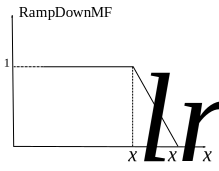
\includegraphics[width=0.3\linewidth]{Chapters/Chapter3/Figures/rampdown_mf.png}}\\[-0.25cm]
	\subfloat[]{\includegraphics[width=0.3\linewidth]{Chapters/Chapter3/Figures/triangle_mf.png}}
	\subfloat[]{\includegraphics[width=0.3\linewidth]{Chapters/Chapter3/Figures/trapezoid_mf.png}}
	\caption{Συναρτήσεις συμμετοχής ασαφούς συνόλου, που χρησιμοποιήθηκαν στον ασαφή ελεγκτή διάσχισης μονοπατιού.}
	\label{fig:membership_functions}
\end{figure}

\bigskip
Η γενική αρχιτεκτονική ενός ελεγκτή ασαφούς λογικής αποτελείται από τέσσερα βασικά τμήματα και τρία στάδια επεξεργασίας. όπως παρουσιάζονται στο σχήμα \ref{fig:fuzzy_controller_architecture}.

\begin{figure}[!ht]
	\centering
	\includegraphics[width=0.6\linewidth]{Chapters/Chapter3/Figures/fuzzy_controller_architecture.png}
	\caption{Γενική Αρχιτεκτονική Ασαφούς Ελεγκτή.}
	\label{fig:fuzzy_controller_architecture}
\end{figure}

\bigskip\noindent
Τα επιμέρους τμήματα της γενικής αρχιτεκτονικής του ελεγκτή ασαφούς λογικής περιγράφονται ως ακολούθως.
\begin{itemize}
	\item Η \textbf{Βάση Γνώσης} (\textit{Knowledge Base}) περιλαμβάνει τις ασαφείς μεταβλητές και τα αντίστοιχα τους ασαφή σύνολα, τα οποία αναπαρίστανται βάσει συναρτήσεων συμμετοχής, όπως επίσης και τους ασαφείς κανόνες, τύπου "if <conditions> then <action>".
	\item Στο στάδιο της \textbf{Aσαφοποίηση} (\textit{Fuzzification}), μία κανονική τιμή (crisp value) μίας ασαφούς μεταβλητής εισόδου ασαφοποιείται σε ζεύγη (ασαφές σύνολο, ποσοστό συμμετοχής), μέσω αντιστοίχισης της τιμής με την συνάρτηση συμμετοχής κάθε ασαφούς συνόλου.
	\item Στο στάδιο του \textbf{Συμπερασμού} (\textit{Inference}), λαμβάνονται οι ασαφείς είσοδοι, εφαρμόζονται οι ασαφείς κανόνες σε αυτούς και παράγεται μία ασαφής έξοδος.
	\item Στο στάδιο της \textbf{Αποασαφοποίησης} (\textit{Defuzzification}), τα ασαφή σύνολα που παράγονται από κάθε κανόνα στο στάδιο του συμπερασμού μετατρέπονται σε κανονικές τιμές, μέσω σταθμισμένου μέσου (weighted average) Takagi-Sugeno:
	\begin{equation}
		WA = \frac{\sum_{i=1}^n \mu(x_i)x_i}{\sum_{i=1}^n \mu(x_i)}
	\end{equation}
\end{itemize}

\subsubsection{Ασαφής Ελεγκτής Διάσχισης Μονοπατιού} \label{sssec:fuzzy_ptc}
Όπως, προαναφέρθηκε, στόχος του αλγορίθμου διάσχισης μονοπατιού, κλειστού βρόχου είναι να ακολουθήσει όσο πιο εύρωστα γίνεται μία διαδρομή, μέσω του ορισμού υπό-στόχων κατά μήκος του μονοπατιού. Επομένως, το μονοπάτι προς διάσχιση αναπαρίσταται ως μία ακολουθία προσανατολισμένων σημείων στο επίπεδο. Επομένως, βάσει ενός μονοπατιού $\left\{p_1, p_2, ..., p_n\right\}$ που πρέπει να ακολουθήσει το ρομπότ για να μεταβεί από μία αρχική κατάσταση $q_I=[x_I, y_I, \theta_I]$ σε ένα στόχο - μία τελική κατάσταση $q_F=[x_F, y_F, \theta_F]$, επιλέγεται ένας υπό-στόχος $q_G=[x_G, y_G, \theta_G]$ πάνω στο εν λόγω μονοπάτι. Σαν αποτέλεσμα, το πρόβλημα της διάσχισης μονοπατιού μετασχηματίζεται σε ένα πρόβλημα προσέγγισης διαδοχικών υπό-στόχων, το οποίο συνεπάγεται έναν νόμο ελέγχου που θα τείνει να μειώνει την απόκλιση μεταξύ του ρομπότ και του τρέχοντα υπό-στόχου, μέχρι τελικά να φτάσει στην επιθυμητή τελική κατάσταση.

\bigskip
Η απόκλιση μεταξύ δύο καταστάσεων στο επίπεδο, μπορεί να οριστεί με διάφορους τρόπους, μέσω ενός συνόλου σφαλμάτων. Μία συνήθης επιλογή, αποτελεί η ευκλείδια απόσταση και το σφάλμα προσανατολισμού μεταξύ δύο καταστάσεων. Στην προκειμένη περίπτωση, για την ικανοποίηση των στόχων του αλγορίθμου διάσχισης μονοπατιού, επιλέχθηκε το ακόλουθο σύνολο τεσσάρων σφαλμάτων που παρουσιάζεται και παραστατικά στο σχήμα \ref{fig:ptc_errors}.

\begin{itemize}
	\item \textbf{$E_o$}:\; Σφάλμα προσανατολισμού μεταξύ κατάστασης ρομπότ και τρέχοντα υπό-στόχου.
	\item \textbf{$E_p$}:\; Σφάλμα απόστασης μεταξύ θέσης ρομπότ και τρέχοντα υπό-στόχου.
	\item \textbf{$E_{a}$}:\; Σφάλμα γωνιακής απόκλισης μεταξύ θέσης ρομπότ και τρέχοντα υπό-στόχου.
	\item \textbf{$E_y$}:\; Σφάλμα πλευρικής απόκλισης μεταξύ θέσης ρομπότ και τρέχοντα υπό-στόχου.
\end{itemize}

\begin{figure}[!ht]
	\centering
	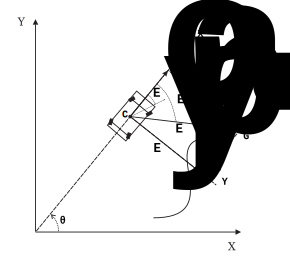
\includegraphics[width=0.5\linewidth]{Chapters/Chapter3/Figures/ptc_errors.png}
	\caption{Σφάλματα μεταξύ τρέχουσας κατάστασης ρομπότ και τρέχοντα υπό-στόχου\\ που επιλέχθηκαν για την υλοποίηση του αλγορίθμου διάσχισης μονοπατιού.}
	\label{fig:ptc_errors}
\end{figure}

\bigskip
Τα σφάλματα $E_o$, $E_p$, $E_a$, $E_y$ χρησιμοποιούνται ως είσοδοι στον ελεγκτή ασαφούς λογικής που σχεδιάστηκε για την ακολούθηση μονοπατιού. Αντίστοιχα, ως έξοδοι του ελεγκτή ορίζονται οι γωνίες $\delta_f$, $\delta_r$ στρέψης των μπροστά και πίσω τροχών και η ταχύτητα $v$ του οχήματος, όπως παρουσιάζεται στο σχήμα \ref{fig:ptc_block_diagram}

\bigskip
\begin{figure}[!ht]
	\centering
	\includegraphics[width=0.8\linewidth]{Chapters/Chapter3/Figures/ptc_block_diagram.png}
	\caption{Βρόχος ελέγχου λειτουργίας διάσχισης μονοπατιού.}
	\label{fig:ptc_block_diagram}
\end{figure}

\bigskip
Επίσης, για την μείωση του απαιτούμενου αριθμού ασαφών κανόνων του προβλήματος ορίζεται η μεταβλητή εισόδου, $Direction$, που δηλώνει την φορά κίνησης συναρτήσει του σφάλματος γωνίας απόκλισης $E_a$ ως

\begin{equation}
	\textit{Direction} =
		\begin{cases}
			-1,\;\; &\text{εάν}\; |E_a| > 120^o\\
			1, \;\; &\text{εάν}\; |E_a| < 120^o
		\end{cases}
\end{equation}

\bigskip
Ο ελεγκτής διάσχισης μονοπατιού αποτελείται από τρεις επιμέρους ανεξάρτητους ελεγκτές, κάθε ένας υπεύθυνος για τον καθορισμό μίας από τις τρεις εξόδους $\delta_f$, $\delta_r$, $v$ του συστήματος. Συγκεκριμένα, οι ελεγκτές παρουσιάζονται στο σχήμα \ref{fig:fuzzy_ptc_inside} και ορίζονται ως ακολούθως.


\begin{figure}[!ht]
	\centering
	\includegraphics[height=8cm]{Chapters/Chapter3/Figures/fuzzy_ptc_inside.png}
	\caption{Ο ελεγκτής διάσχισης μονοπατιού.}
	\label{fig:fuzzy_ptc_inside}
\end{figure}

\begin{itemize}
	\item Ο \textbf{ασαφής ελεγκτής ταχύτητας} (\textbf{Speed Fuzzy Logic Controller}) παίρνει ως είσοδο το σφάλμα θέσης $E_p$ και την φορά κίνησης $Direction$ και παρέχει ως έξοδο την ταχύτητα $v$ κίνησης του ρομπότ.

	\item Ο \textbf{ασαφής ελεγκτής μπροστινοδιεύθυνσης} (\textbf{Front Steering Fuzzy Logic Controller}) παίρνει ως είσοδο τα σφάλματα $E_o$, $E_a$, $E_p$ και την φορά κίνησης $Direction$ και παράγει ως έξοδος την γωνία στρέψης $\delta_f$ των μπροστινών τροχών.
	
	\item Ο \textbf{ασαφής ελεγκτής απόκλισης πισωδιεύθυνσης} (\textbf{Rear Steering Deviation Fuzzy Logic Controller}) παίρνει ως είσοδο τα σφάλματα $E_o$, $E_y$ και την φορά κίνησης $Direction$ και παράγει την επιθυμητή γωνία απόκλισης της γωνίας στρέψης των πίσω τροχών από την αντίθετη γωνία στρέψης των μπροστινών τροχών. Επομένως, η γωνία στρέψης των πίσω τροχών προκύπτει ως 
	
\begin{equation}
	\delta_r = - \delta_f + \alpha_r	
\end{equation}

\end{itemize}


\bigskip
Στη συνέχεια για κάθε μία από τις εισόδους του ελεγκτή ορίζονται ένα σύνολο ασαφών συνόλων και οι αντίστοιχες συναρτήσεις συμμετοχής, όπως παρουσιάζεται στο σχήμα \ref{fig:ptc_input_mfs}.

\bigskip
\begin{figure}[!ht]
	\centering
	\subfloat[$\mu_{Eo}\; \text{και}\; \mu_{Ea}$]{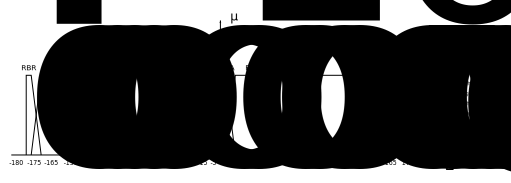
\includegraphics[height=0.3\linewidth]{Chapters/Chapter3/Figures/eo_ea_mf.png}}\\
	\subfloat[$\mu_{Ep}$]{\includegraphics[height=0.3\linewidth]{Chapters/Chapter3/Figures/ep_mf.png}}
	\subfloat[$\mu_{Ey}$]{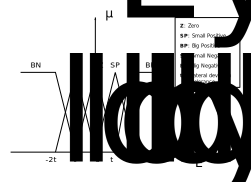
\includegraphics[height=0.3\linewidth]{Chapters/Chapter3/Figures/ey_mf.png}}
	\subfloat[$\mu_{Direction}$]{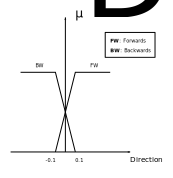
\includegraphics[height=0.3\linewidth]{Chapters/Chapter3/Figures/direction_mf.png}}
	\caption{Οι συναρτήσεις συμμετοχής των μεταβλητών εισόδου του ελεγκτή διάσχισης μονοπατιού.}
	\label{fig:ptc_input_mfs}
\end{figure}

\bigskip
Αντίστοιχα, ορίζονται και τα ασαφή σύνολα των εξόδων του ελεγκτή διάσχισης μονοπατιού, όπως παρουσιάζεται στο σχήμα \ref{fig:ptc_output_mfs}.

\bigskip
\begin{figure}[!ht]
	\centering
	\subfloat[$\mu_{speed}$]{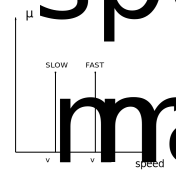
\includegraphics[height=0.3\linewidth]{Chapters/Chapter3/Figures/speed_mf.png}}
	\subfloat[$\mu_{FSA}\; \text{και}\; \mu_{RSA}$]{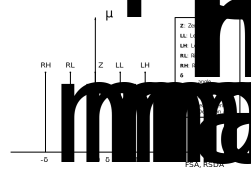
\includegraphics[height=0.3\linewidth]{Chapters/Chapter3/Figures/df_dr_mf.png}}\\
	\caption{Οι συναρτήσεις συμμετοχής των μεταβλητών εξόδου του ελεγκτή διάσχισης μονοπατιού.}
	\label{fig:ptc_output_mfs}
\end{figure}

\bigskip
Έχοντας ορίσει τις μεταβλητές εισόδου, εξόδου και τα αντίστοιχα ασαφή σύνολα και συναρτήσεις συμμετοχής, το μόνο που μένει είναι ο ορισμός των ασαφών κανόνων της βάση γνώσης του ελεγκτή. Η επιλογή των ασαφών κανόνων των τριών επιμέρους ελεγκτών του ελεγκτή διάσχισης μονοπατιού, πραγματοποιήθηκε βάσει της επιθυμητής συμπεριφοράς του ελεγκτή ανά ένα σύνολο περιπτώσεων. Οι περιπτώσεις που πρέπει ικανοποιούν οι ασαφείς κανόνες έχουν ως εξής:

\begin{enumerate}
	\item Η ταχύτητα θα πρέπει να είναι η μέγιστη δυνατή, όταν το όχημα βρίσκεται μακρυά από τον στόχο και να ελαττώνεται όταν πλησιάζει σ' αυτόν.
	\item Στην περίπτωση που το όχημα βρίσκεται μακρυά από τον στόχο θα πρέπει η γωνία στρέψης των μπροστινών τροχών να στρέφεται ανάλογα με το μέγεθος και την κατεύθυνση του σφάλματος γωνιακής απόκλισης. Γι αυτήν την περίπτωση δεν μας ενδιαφέρει, τόσο το σφάλμα προσανατολισμού, όσο η προσέγγιση του στόχου.
	\item Στην περίπτωση που το όχημα βρίσκεται κοντά στον στόχο, αντιθέτως, δεν μας ενδιαφέρει η προσέγγιση του στόχου, μιας και είμαστε είδη κοντά, αλλά η διόρθωση του σφάλματος προσανατολισμού.
	\item Στην περίπτωση που το σφάλμα προσανατολισμού είναι μικρό και η πλευρική απόκλιση δεν είναι εξαιρετικά μεγάλη, θα πρέπει η απόκλιση της γωνίας στρέψης των πίσω τροχών να είναι μεγάλη, ούτως ώστε, το όχημα να κινείται με θετική τετραδιεύθυνση, κρατώντας το σφάλμα προσανατολισμού μικρό. Η περίπτωση αυτή είναι χρήσιμη για την περίπτωση ολίσθησης ή για διόρθωση μικρής πλευρικής απόκλισης.
	\item Σε περίπτωση που το σφάλμα προσανατολισμού είναι μικρό, αλλά το σφάλμα πλευρικής απόκλισης είναι πολύ μεγάλο τότε θα πρέπει η απόκλιση της γωνίας στρέψης των πίσω τροχών να είναι μηδενική, ούτως ώστε, το όχημα να κινείται με αρνητική τετραδιεύθυνση, με στόχο την προσέγγιση του μονοπατιού, διορθώνοντας το σφάλμα γωνιακής απόκλισης και πλευρικής απόκλισης, χωρίς να λαμβάνεται υπόψιν το σφάλμα προσανατολισμού.
	\item Ο ελεγκτής θα πρέπει να μπορεί να ικανοποιεί τις παραπάνω περιπτώσεις και για τις δύο δυνατές φορές κίνησης, εμπρός και πίσω.
\end{enumerate}

\begin{table}[!ht]
	\centering
	\captionof{table}{Οι ασαφείς κανόνες του ελεγκτή ταχύτητας.}
	\label{tab:speed_fuzzy_rules}
	\begin{tabular}{| l | l |}
		\hline
	   \rotatebox[origin=c]{90}{\textbf{\,Speed Fuzzy Rules\,}} &
	   %------------------
		\begin{tabular}{l}
		   if Ep is CLOSE then Speed is SLOW\\
   			if Ep is FAR then Speed is FAST
   		\end{tabular}\\ \hline
   	\end{tabular}
\end{table}

\begin{table}[!ht]
	\centering
	\captionof{table}{Οι ασαφείς κανόνες του ελεγκτή της γωνίας στρέψης των μπροστινών τροχών.}
	\label{tab:fsa_fuzzy_rules}
	\begin{tabular}{| c | l |}
		\hline
	   \rotatebox[origin=c]{90}{\textbf{FSA Fuzzy Rules}} &
	   %----------------------
   		\begin{tabular}{l}
	   if Ep is FAR and Ea is RBL then FSA is  Z\\
      if Ep is FAR and Ea is  RL then FSA is LH\\
      if Ep is FAR and Ea is  SL then FSA is LH\\
      if Ep is FAR and Ea is  FL then FSA is LL\\
      if Ep is FAR and Ea is  FA then FSA is  Z\\
      if Ep is FAR and Ea is  FR then FSA is RL\\
      if Ep is FAR and Ea is  SR then FSA is RH\\
      if Ep is FAR and Ea is  RR then FSA is RH\\
    	if Ep is FAR and Ea is RBR then FSA is  Z\\
	   if Ep is CLOSE and Direction is FW and Eo is SL then FSA is LH\\
    	if Ep is CLOSE and Direction is FW and Eo is FL then FSA is LL\\
    	if Ep is CLOSE and Direction is FW and Eo is FA then FSA is Z\\
    	if Ep is CLOSE and Direction is FW and Eo is FR then FSA is RL\\
    	if Ep is CLOSE and Direction is FW and Eo is SR then FSA is RH\\
   		if Ep is CLOSE and Direction is BW and Eo is SL then FSA is RH\\
	   if Ep is CLOSE and Direction is BW and Eo is FL then FSA is RL\\
	   if Ep is CLOSE and Direction is BW and Eo is FR then FSA is LL\\
    	if Ep is CLOSE and Direction is BW and Eo is SR then FSA is LH
		\end{tabular}\\ \hline
	\end{tabular}
\end{table}

\begin{table}[!ht]
	\centering
	\captionof{table}{Οι ασαφείς κανόνες του ελεγκτή της απόκλισης της γωνίας στρέψης των πίσω τροχών.}
	\label{tab:rsda_fuzzy_rules}
	\begin{tabular}{| c | l |}
		\hline
	   \rotatebox[origin=c]{90}{\textbf{RSDA Fuzzy Rules}} &
	   %----------------------
		\begin{tabular}{l}
    	if Eo is not FA and Eo is not FR and Eo is not FL then RSDA is Z\\
    	if Direction is FW and Eo is FA and Ey is BP then RSDA is  Z\\
    	if Direction is FW and Eo is FL and Ey is BP then RSDA is  Z\\
    	if Direction is FW and Eo is FR and Ey is BP then RSDA is  Z\\
    	if Direction is FW and Eo is FA and Ey is SP then RSDA is LH\\
    	if Direction is FW and Eo is FL and Ey is SP then RSDA is LH\\
    	if Direction is FW and Eo is FR and Ey is SP then RSDA is LH\\
    	if Direction is FW and Eo is FA and Ey is  Z then RSDA is  Z\\
    	if Direction is FW and Eo is FL and Ey is  Z then RSDA is  Z\\
    	if Direction is FW and Eo is FR and Ey is  Z then RSDA is  Z\\
    	if Direction is FW and Eo is FA and Ey is SN then RSDA is RH\\
    	if Direction is FW and Eo is FL and Ey is SN then RSDA is RH\\
    	if Direction is FW and Eo is FR and Ey is SN then RSDA is RH\\
    	if Direction is FW and Eo is FA and Ey is BN then RSDA is  Z\\
    	if Direction is FW and Eo is FL and Ey is BN then RSDA is  Z\\
    	if Direction is FW and Eo is FR and Ey is BN then RSDA is  Z\\
    	if Direction is BW and Eo is FA and Ey is BP then RSDA is  Z\\
    	if Direction is BW and Eo is FL and Ey is BP then RSDA is  Z\\
    	if Direction is BW and Eo is FR and Ey is BP then RSDA is  Z\\
	   	if Direction is BW and Eo is FA and Ey is SP then RSDA is LH\\
    	if Direction is BW and Eo is FL and Ey is SP then RSDA is LH\\
    	if Direction is BW and Eo is FR and Ey is SP then RSDA is LH\\
    	if Direction is BW and Eo is FA and Ey is  Z then RSDA is  Z\\
    	if Direction is BW and Eo is FL and Ey is  Z then RSDA is  Z\\
    	if Direction is BW and Eo is FR and Ey is  Z then RSDA is  Z\\
    	if Direction is BW and Eo is FA and Ey is SN then RSDA is RH\\
    	if Direction is BW and Eo is FL and Ey is SN then RSDA is RH\\
    	if Direction is BW and Eo is FR and Ey is SN then RSDA is RH\\
    	if Direction is BW and Eo is FA and Ey is BN then RSDA is  Z\\
    	if Direction is BW and Eo is FL and Ey is BN then RSDA is  Z\\
    	if Direction is BW and Eo is FR and Ey is BN then RSDA is  Z
    	\end{tabular}\\ \hline
	\end{tabular}
\end{table}

%%%%%%%%%%%%%%%%%%%%%%%%%%%%%%%%%%%%%%%%%%%%%%%%%%%%%%%%%%%%%%%%%%%%%%%%%%%%%%%%%%%%%%%%%%%%%%
%\begin{figure}[!ht]
%	\centering
%	\includegraphics[width=\linewidth]{Chapters/Chapter3/Figures/.png}
%	\caption[]{ \cite{}.}
%	\label{fig:}
%\end{figure}

%% Chapter Template

\chapter{Αρχιτεκτονική Συστήματος} % Main chapter title

\label{Chapter4} % Change X to a consecutive number; for referencing this chapter elsewhere, use \ref{ChapterX}


%----------------------------------------------------------------------------------------
%	SECTION 1: ROS
%----------------------------------------------------------------------------------------
\section{ROS}


%----------------------------------------------------------------------------------------
%	SECTION 2: Simulation Tools
%----------------------------------------------------------------------------------------
\section{Εργαλεία Προσομοίωσης}
\subsection{STDR - 2D Προσομοίωση}
\subsection{GAZEBO - 3D Προσομοίωση}


%----------------------------------------------------------------------------------------
%	SECTION 3: Software Architecture 
%----------------------------------------------------------------------------------------
\section{Αρχιτεκτονική Λογισμικού}
%
\chapter{Πειράματα και Αποτελέσματα} \label{Chapter5}
Στο παρόν κεφάλαιο παρουσιάζονται τα πειράματα και τα αποτελέσματα που πραγματοποιήθηκαν για την επαλήθευση και την αξιολόγηση της συμπεριφοράς των υποσυστημάτων της ρομποτικής πλατφόρμας Monstertruck, σε σχέση με την επιθυμητή. Παράλληλα, πραγματοποιείται και σύγκριση μεταξύ των διαφορετικών εκδοχών ορισμένων υποσυστημάτων, όπως αυτά παρουσιάστηκαν στο Κεφάλαιο \ref{Chapter4}. 

\bigskip
Η εκτέλεση των πειραμάτων πραγματοποιήθηκε, μέσω προσομοίωσης σε δύο διαστάσεις με τον προσομοιωτή STDR, σε τρεις διαστάσεις με τον προσομοιωτή Gazebo, όπως επίσης και στο φυσικό ρομπότ που αναπτύχθηκε στα πλαίσια της παρούσας διπλωματικής. Τα εν λόγω πειράματα εκτελέστηκαν σε επίπεδο προσομοίωσης σε έναν υπολογιστή με επεξεργαστή Intel Core i5 2.4GHz, 6GB RAM και κάρτα γραφικών NVIDIA GeForce GT330M, ενώ σε επίπεδο φυσικού ρομπότ σε έναν υπολογιστή ODROID-XU4 με προδιαγραφές, όπως αυτές παρουσιάστηκαν στον πίνακα \ref{tab:computer_specs}, όπου και τα δύο υπολογιστικά συστήματα έτρεχαν το λειτουργικό σύστημα Ubuntu 14.04, σε συνδυασμό με το αντίστοιχο συμβατό meta-λειτουργικό σύστημα ROS Indigo Igloo.

\bigskip
Στην συνέχεια παρουσιάζονται τα πειράματα και τα αποτελέσματα που πραγματοποιήθηκαν για την επαλήθευση και αξιολόγηση του κινηματικού μοντέλου, των συστημάτων χαρτογράφησης και εντοπισμού θέσης, των συστημάτων κατασκευής μονοπατιού, αποφυγής εμποδίων και διάσχισης μονοπατιού, ενώ τελικά γίνεται και μία αξιολόγηση της αυτόνομης συμπεριφοράς του ρομπότ, αλλά και της απόδοσης του υπολογιστή του ρομπότ, όσον αφορά τους πόρους που δεσμεύονται από κάθε διεργασία ξεχωριστά και όλων μαζί.

%----------------------------------------------------------------------------------------
%	SECTION 1: Kinematics Experiments
%----------------------------------------------------------------------------------------
\section{Πειράματα Κινηματικού Μοντέλου} \label{sec:kinematics_experiments}  %TODO for real robot
Η αξιολόγηση του κινηματικού μοντέλου που αναπτύχθηκε για την ρομποτική πλατφόρμα Monstertruck, πραγματοποιήθηκε, αρχικά, στον προσομοιωτή Gazebo και έπειτα στο φυσικό ρομπότ, μέσα από μία σειρά πειραμάτων με στόχο την σύγκριση της ιδανικής με την πραγματική συμπεριφορά του ρομπότ.  

\bigskip
Για την εκτέλεση των πειραμάτων, κρίθηκε σκόπιμο να χρησιμοποιηθούν χώροι, αρκετά μικροί, ούτως ώστε να επιτρέπουν την χαρτογράφηση και τον εντοπισμό θέσης του ρομπότ, βάσει της εμβέλειας του σαρωτή λέιζερ Hokuyo URG-04LX, ενώ παράλληλα να είναι αρκετά μεγάλοι, ώστε να επιτρέπουν την εκτέλεση των επιθυμητών τροχιών από το ρομπότ. Επίσης, κρίθηκε σκόπιμο να χρησιμοποιηθούν χώροι με επίπεδο και ομαλό έδαφος, για την πιο αξιόπιστη εκτέλεση των πειραμάτων, χωρίς την εισαγωγή διαταραχών, λόγω ανώμαλου εδάφους ή ολίσθησης σε κεκλιμένο επίπεδο. Συγκεκριμένα, για την εκτέλεση των πειραμάτων στον προσομοιωτή Gazebo αναπτύχθηκε το περιβάλλον \textit{simple{\_}room} που αποτελείται από ένα απλό δωμάτιο $4m \times 4m \times 1.5m$ με τέσσερις τοίχους και επίπεδο και ομαλό έδαφος, όπως αυτό παρουσιάζεται στην εικόνα \ref{fig:simple_room}, ενώ τα πειράματα στο φυσικό ρομπότ πραγματοποιήθηκαν στην πίστα πειραμάτων του εργαστηρίου της ομάδας P.A.N.D.O.R.A, όπως παρουσιάζεται στην εικόνα \ref{fig:pandora_circuit}.

\begin{figure}[!ht]
	\centering
	\frame{\includegraphics[width=\linewidth]{Chapters/Chapter5/Figures/simple_room.png}}
	\caption{Το περιβάλλον simple{\_}room που χρησιμοποιήθηκε για την εκτέλεση πειραμάτων  αξιολόγησης του κινηματικού μοντέλου στον προσομοιωτή Gazebo.}
	\label{fig:simple_room}
\end{figure}

\begin{figure}[!ht]
	\centering
	\includegraphics[width=\linewidth]{Chapters/Chapter5/Figures/pandora_arena.jpg}
	\caption{Η πίστα του εργαστηρίου της ομάδας P.A.N.D.O.R.A που χρησιμοποιήθηκε για την εκτέλεση πειραμάτων στο φυσικό ρομπότ για την αξιολόγηση του κινηματικού μοντέλου.}
	\label{fig:pandora_circuit}
\end{figure}

\bigskip
Για την εκτέλεση των πειραμάτων χρησιμοποιήθηκε το σύστημα χαρτογράφησης και εντοπισμού θέσης με τον αλγόριθμο CRSM-SLAM, ενώ ο έλεγχος του ρομπότ έγινε μέσω τηλεχειρισμού. Για την αξιολόγηση της συμπεριφοράς του ρομπότ, χρησιμοποιήθηκαν οι εντολές κίνησης που δόθηκαν στο ρομπότ, ως η επιθυμητή συμπεριφορά και η πραγματική τροχιά του ρομπότ, που εκδίδει ο αλγόριθμος CRSM-SLAM, ως η πραγματική συμπεριφορά.

\bigskip
Συνολικά, πραγματοποιήθηκαν δύο είδη πειραμάτων για την αξιολόγηση του κινηματικού μοντέλου και συγκεκριμένα για την αξιολόγηση της ακτίνας τροχιάς κατά την εκτέλεση κυκλικών τροχιών με αρνητική τετραδιεύθυνση και για την αξιολόγηση της πλευρικής γωνίας ολίσθησης κατά την εκτέλεση διαγώνιων ευθύγραμμων τροχιών με θετική τετραδιεύθυνση, όπως αυτά παρουσιάζονται στην συνέχεια.

\subsection{Τροχιές Αρνητικής Τετραδιεύθυνσης}
Για την αξιολόγηση της αρνητικής τετραδιεύθυνσης πραγματοποιήθηκε μία σειρά πειραμάτων, στην οποία, δόθηκαν εντολές στο ρομπότ για εκτέλεση κυκλικών τροχιών, για διάφορες δυνατές γωνίες στρέψης των τροχών, για τις οποίες, έπειτα υπολογίστηκαν οι ιδανικές ακτίνες τροχιάς $R_{ideal}$ και οι πραγματικές $R_{sim}$ και $R_{real}$, προσομοίωσης και φυσικού ρομπότ αντίστοιχα, όπως αυτές παρουσιάζονται στον πίνακα \ref{tab:counter_steering_experiment} και στο σχήμα \ref{fig:counter_steering_experiment}. Με βάση τον πίνακα αυτόν, παρατηρείται μία μικρή απόκλιση των πραγματικών τροχιών που εκτελεί το ρομπότ σε σύγκριση με τις ιδανικές, κάτι που, παρόλα αυτά, είναι δικαιολογημένο, λόγω της μη ιδανικότητας του κινηματικού μοντέλου τετραδιεύθυνσης της ρομποτικής πλατφόρμας Monstertruck, όπως επίσης και την επιρροή φαινομένων τριβών και ολίσθησης στους τροχούς.
 
\begin{table}[!ht]
	\centering
	\captionof{table}{Αποτελέσματα πειράματος κινηματικού σε τροχιές αρνητικής τετραδιεύθυνσης.}
	\label{tab:counter_steering_experiment}
	\begin{tabular}{c | c |  c | c}
	 	\textbf{$\delta_f$}, \textbf{$-\delta_r$} & \textbf{$R_{ideal}$} & \textbf{$R_{sim}$} & \textbf{$R_{real}$} \\ \hline
	   %------------------------------------------------------------------------------
	   $0.4$ & $0.378$ & $0.377$ & $0.396$\\
 	   $0.32$ & $0.483$ & $0.519$ & $0.524$\\
  	   $0.24$ & $0.654$ & $0.722$ & $0.689$\\
   	   $0.16$ & $0.991$ & $1.023$ & $1.087$
   	\end{tabular}
\end{table}

\begin{figure}[!ht]
	\centering
	\subfloat[]{\frame{\includegraphics[height=7cm]{Chapters/Chapter5/Figures/counter_steering_experiment.png}}} \hspace{1cm}
	\subfloat[]{\frame{\includegraphics[height=7cm]{Chapters/Chapter5/Figures/counter_steering_experiment_real.png}}}
	\caption{Τροχιές που παράχθηκαν κατά τα πειράματα αξιολόγησης του κινηματικού μοντέλου σε τροχιές αρνητικής τετραδιεύθυνσης στα περιβάλλοντα (α') simple{\_}room και (β') πίστα της ομάδας P.A.N.D.O.R.A.}
	\label{fig:counter_steering_experiment}
\end{figure}


\subsection{Τροχιές Θετικής Τετραδιεύθυνσης}
Για την αξιολόγηση της θετικής τετραδιεύθυνσης πραγματοποιήθηκε μία σειρά πειραμάτων, στην οποία, δόθηκαν εντολές στο ρομπότ για εκτέλεση διαγώνιων τροχιών, για διάφορες δυνατές γωνίες στρέψης των τροχών $\delta_f$, $\delta_r$, τέτοιες ώστε $\delta_f = \delta_r$, ενώ, έπειτα, υπολογίστηκε η ιδανική γωνία πλευρικής ολίσθησης $\beta_{ideal}$, όπως επίσης και οι πραγματικές γωνίες πλευρικής ολίσθησης $\beta_{sim}$ και $\beta_{real}$ των πραγματικών τροχιών που εκτελέστηκαν από το ρομπότ σε επίπεδο προσομοίωσης και επίπεδο φυσικού ρομπότ αντίστοιχα και οι οποίες παρουσιάζονται στον πίνακα \ref{tab:crab_steering_experiment} και στο σχήμα \ref{fig:crab_steering_experiment}. Παρατηρείται, γενικά, πολύ μικρό έως αμελητέο σφάλμα της πραγματικής συμπεριφοράς του ρομπότ σε σύγκριση με την ιδανική και επομένως, αυτή, κρίνεται πλήρως αποδεκτή.

\bigskip 
\begin{table}[!ht]
	\centering
	\captionof{table}{Αποτελέσματα πειράματος κινηματικού σε τροχιές θετικής τετραδιεύθυνσης.}
	\label{tab:crab_steering_experiment}
	\begin{tabular}{c | c |  c | c}
	 	\textbf{$\delta_f$, $\delta_r$} & \textbf{$\beta_{ideal}$} & \textbf{$\beta_{sim}$} & \textbf{$\beta_{real}$} \\ \hline
	   %------------------------------------------------------------------------------
	   $0.4$ & $0.4$ & $0.398$ & $0.427$\\
 	   $0.32$ & $0.32$ & $0.326$ & $0.338$\\
  	   $0.24$ & $0.24$ & $0.232$ & $0.246$\\
   	   $0.16$ & $0.16$ & $0.151$ & $0.139$\\
   	\end{tabular}
\end{table}

\begin{figure}[!ht]
	\centering
	\subfloat[]{\frame{\includegraphics[height=6.5cm]{Chapters/Chapter5/Figures/crab_steering_experiment.png}}} \hspace{0.75cm}
	\subfloat[]{\frame{\includegraphics[height=6.5cm]{Chapters/Chapter5/Figures/crab_steering_experiment_real.png}}}
	\caption{Τροχιές που παράχθηκαν κατά τα πειράματα αξιολόγησης του κινηματικού μοντέλου σε τροχιές θετικής τετραδιεύθυνσης στα περιβάλλοντα (α´) simple{\_}room και (β') πίστα της ομάδας P.A.N.D.O.R.A.}
	\label{fig:crab_steering_experiment}
\end{figure}


%----------------------------------------------------------------------------------------
%	SECTION 2: SLAM Experiments
%----------------------------------------------------------------------------------------
\section{Πειράματα Χαρτογράφησης} \label{sec:slam_experiments}
Στην παρούσα ενότητα γίνεται μία αξιολόγηση των συστημάτων χαρτογράφησης και υπολογισμού θέσης, όπως αυτά παρουσιάσθηκαν στην ενότητα \ref{ssec:slam_components}, μέσω σύγκρισης των δύο επιμέρους συστημάτων, αλλά και μέσω σύγκρισης με τον πραγματικό χάρτη, εφόσον αυτός παρέχεται. Τα πειράματα πραγματοποιήθηκαν στον 2D προσομοιωτή STDR, στον 3D προσομοιωτή Gazebo, αλλά και στο φυσικό ρομπότ, με χρήση των συστημάτων χαρτογράφησης και εντοπισμού θέσης των αλγορίθμων CRSM-SLAM και Gmapping.

\bigskip
Για την χαρτογράφηση του περιβάλλοντος, η ρομποτική πλατφόρμα Monstertruck χρησιμοποιεί ως βασικό εργαλείο τον σαρωτή λέιζερ Hokuyo URG-04LX, ο οποίος έχει εμβέλεια $4m$ και επομένως τα περιβάλλοντα των πειραμάτων επιλέχθηκαν αναλόγως. Συγκεκριμένα, επιλέχθηκαν περιβάλλοντα με εσωτερικούς κλειστούς χώρους, με αρκετά στενούς διαδρόμους και δωμάτια με επαρκή ποικιλομορφία για την όσο το δυνατόν πιο αξιόπιστη χαρτογράφηση. Επίσης, λόγω της περιορισμένης υπολογιστικής ισχύς του υπολογιστή ODROID-XU4, της ρομποτικής πλατφόρμας Monstertruck, επιλέχθηκε ανάλυση χαρτογράφησης ίση με $0.04m$ και γενικότερα ειδική παραμετροποίηση των αλγορίθμων SLAM, έτσι ώστε να επιτευχθεί ταυτόχρονα αύξηση της συχνότητας ανανέωσης του χάρτη και μείωση του υπολογιστικού φόρτου, με εμφανή επίδραση, παρόλα αυτά, στην ποιότητα του.

\subsection{Χαρτογράφηση στον 2D Προσομοιωτή STDR} \label{ssec:stdr_slam}
%------------------------------------------------%
Για τα πειράματα στον προσομοιωτή STDR, επιλέχθηκε ο χάρτης \textit{robocup} που παρέχεται από τον προσομοιωτή, λόγω της πολυπλοκότητας του και της ομοιότητας του με τα περιβάλλοντα για τα οποία προορίζεται η ρομποτική πλατφόρμα Monstertruck. Παρόλα αυτά, μετά από αρχικά πειράματα, διαπιστώθηκε ότι ο χάρτης είχε κάποιους μεγάλους ομοιόμορφους διαδρόμους που δημιουργούσαν πρόβλημα στην χαρτογράφηση, με τον αλγόριθμο CRSM-SLAM, λόγω αδυναμίας εντοπισμού της ακριβής θέσης, εξαιτίας του περιορισμένου εύρους του σαρωτή λέιζερ και άρα της εσφαλμένης αντιστοίχισης σκαναρισμάτων. Γι αυτό το λόγο, κρίθηκε σκόπιμο να μειωθεί η ανάλυση του χάρτη από $0.03$ σε $0.02$ με στόχο την μείωση της κλίμακας του. Στο σχήμα \ref{fig:stdr_robocup} παρουσιάζεται ο χάρτης robocup και οι αντίστοιχοι χάρτες που κατασκεύασαν οι αλγόριθμοι CRSM-SLAM και Gmapping.

\begin{figure}[!ht]
	\centering
	\subfloat[Ground Truth.]{\includegraphics[width=0.31\linewidth, height=5cm]{Chapters/Chapter5/Figures/stdr_robocup_ground_truth.png}}
	\subfloat[CRSM-SLAM]{\includegraphics[width=0.31\linewidth, height=5cm]{Chapters/Chapter5/Figures/stdr_robocup_crsm.png}}
	\subfloat[Gmapping]{\includegraphics[width=0.31\linewidth, height=5cm]{Chapters/Chapter5/Figures/stdr_robocup_gmapping.png}}
	\caption{Χάρτες του περιβάλλοντος robocup.}
	\label{fig:stdr_robocup}
\end{figure}

\bigskip
Βάσει του σχήματος \ref{fig:stdr_robocup}, παρατηρείται, ότι τα δύο συστήματα χαρτογράφησης που εξετάστηκαν, παράγουν μία αναπαράσταση του περιβάλλοντος robocup, με αρκετές ατέλειες, αλλά χωρίς να υπάρχει κάποιο εξαιρετικά μεγάλο σφάλμα που να επιδρά σημαντικά στην ακεραιότητα του χάρτη και επομένως κρίνονται ικανοποιητικά για τα πλαίσια της παρούσας εργασίας.

\subsection{Χαρτογράφηση στον 3D προσομοιωτή Gazebo} \label{ssec:gazebo_slam}
%--------------------------------------------------%
Για τα πειράματα χαρτογράφησης στον προσομοιωτή Gazebo, επιλέχθηκε ο χάρτης της αρένας του διαγωνισμού RoboCup Rescue 2013, σε δύο εκδοχές, με ομαλό και ανώμαλο έδαφος για την εξέταση της συμπεριφοράς του συστήματος, υπό όλες τις δυνατές συνθήκες για τις οποίες προορίζεται να λειτουργήσει αυτό.

\bigskip
Για την διεξαγωγή των πειραμάτων, το ρομπότ τέθηκε σε λειτουργία αυτόματης εξερεύνησης χωρίς κάποια χειροκίνητη παρέμβαση, για την κάλυψη όλης της αρένας για τις περιπτώσεις ομαλού και ανώμαλου εδάφους, με στόχο την πλήρη χαρτογράφηση αυτών, μέσω των αλγορίθμων CRSM-SLAM και Gmapping.

\subsubsection{Χαρτογράφηση της Αρένας RoboCup Rescue 2013 με Ομαλό Έδαφος}
Για την χαρτογράφηση, σε ομαλό έδαφος, η αρένα RoboCup Rescue 2013 προσαρμόστηκε κατάλληλα για να επιτρέπει την πλήρη προσπέλαση της από το ρομπότ, μέσω της αφαίρεσης ανυψωμένων τμημάτων, όπως ράμπες, σκάλες κοκ. Στο σχήμα \ref{fig:robocup_2013_arena_flat} παρουσιάζεται η προσαρμοσμένη αρένα RoboCup Rescue 2013, με ομαλό έδαφος, όπως επίσης και οι αντίστοιχοι χάρτες που κατασκευάστηκαν από τους αλγορίθμους CRSM-SLAM και Gmapping.

\bigskip
Συγκρίνοντας, τους παραγόμενους χάρτες με το πραγματικό περιβάλλον παρατηρούνται κάποια σφάλματα συστροφής μεταξύ των οριζόντιων διαδρόμων της αρένας, που παρόλα αυτά, δεν επιδρούν σημαντικά στην ακεραιότητα του χάρτη. Τα δύο συστήματα χαρτογράφησης κατασκεύασαν επαρκείς αναπαραστάσεις της αρένας, με ελαφρώς καλύτερη αυτή του αλγορίθμου Gmapping, εις βάρος, παρόλα αυτά του υπολογιστικού φόρτου και των απαιτήσεων αυτού. 

\subsubsection{Χαρτογράφηση της Αρένας RoboCup Rescue 2013 με Ανώμαλο Έδαφος}
Για την περίπτωση της αρένας με ανώμαλο έδαφος, χρησιμοποιήθηκε αρχικά η ακέραιη εκδοχή της αρένας RoboCup Rescue 2013, αλλά παρατηρήθηκε ότι περιείχε τμήματα τα οποία δεν ήταν δυνατόν να γίνουν αντιληπτά, ενώ παράλληλα δεν ήταν ούτε προσπελάσιμα από το ρομπότ. Επομένως, κρίθηκε σκόπιμο, η εν λόγω αρένα να προσαρμοστεί, ούτως ώστε να αφαιρεθούν τα τμήματα αυτά. Συγκεκριμένα, αφαιρέθηκαν από την αρένα τα ακόλουθα τμήματα, όπως αυτά παρουσιάζονται ακολούθως και στο σχήμα \ref{fig:removed_parts_from_robocup_arena}:

\begin{itemize}
	\item Μία σκάλα, η οποία είχε κενό μεταξύ των σκαλοπατιών, με αποτέλεσμα να περνάνε διαμέσου αυτής οι ακτίνες του σαρωτή λέιζερ και άρα αυτήν να γίνεται αντιληπτή εσφαλμένα ως ελεύθερος χώρος.
	\item Μία ράμπα μεγάλης κλίσης, της οποίας το κατώτερο τμήμα δεν αναγνωριζόταν ως εμπόδιο, με κίνδυνο σύγκρουσης με το ρομπότ.
	\item Ένα σύνολο τμημάτων με υψηλά και άνισα κομμάτια που προεξείχαν σε αρκετά χαμηλό ύψος, ώστε να μην χτυπάνε οι ακτίνες του λέιζερ σ' αυτά, αλλά παράλληλα αρκετά ψηλά, ώστε να προκαλούν την προσκόλληση ή ακόμα και ανατροπή του ρομπότ.
\end{itemize}

\begin{figure}[!ht]
	\subfloat[Σκάλα.]{\includegraphics[width=0.32\linewidth, height=3.5cm]{Chapters/Chapter5/Figures/staircase.png}}
	\hspace{0.01\linewidth}
	\subfloat[Ράμπα μεγάλης κλίσης.]{\includegraphics[width=0.32\linewidth, height=3.5cm]{Chapters/Chapter5/Figures/big_ramp.png}}
	\hspace{0.01\linewidth}
	\subfloat[Μη αντιλήψιμα - μη προσπελάσιμα εμπόδια.]{\includegraphics[width=0.32\linewidth, height=3.5cm]{Chapters/Chapter5/Figures/stepfield.png}}
	\caption{Τα τμήματα που αφαιρέθηκαν από την αρένα με το ανώμαλο έδαφος, λόγω της αδυναμίας εντοπισμού και προσπελασιμότητας από την ρομποτική πλατφόρμα Monstertruck.}
	\label{fig:removed_parts_from_robocup_arena}
\end{figure}

\bigskip
Αφού αφαιρεθούν τα παραπάνω εμπόδια από τον χάρτη, το ανώμαλο έδαφος προσεγγίζεται, πλέον, με ξύλινες ράμπες με κλίση περίπου $15^o$. Η αξιόπιστη χαρτογράφηση περιβάλλοντος, αυτού του τύπου, καθίσταται δυνατή από την αντιστάθμιση κλίσης roll και pitch του σαρωτή λέιζερ, μέσω του μηχανισμού σταθεροποίησης αυτού, σε συνδυασμό με την πυξίδα που παρέχει τις μετρήσεις των κλίσεων roll και pitch του ρομπότ. Στα σχήματα \ref{fig:robocup_2013_arena} που ακολουθούν, παρουσιάζεται η προσαρμοσμένη αρένα και οι αντίστοιχοι χάρτες.

\bigskip
Οι χάρτες που κατασκεύασαν τα δύο συστήματα SLAM για την αρένα με το ανώμαλο έδαφος παρουσιάζουν εξαιρετικά μεγάλη ομοιότητα με τους αντίστοιχους χάρτες της αρένας με το ομαλό έδαφος, γεγονός που αποδεικνύει την ευρωστία του συστήματος σε όλες τις πιθανές συνθήκες λειτουργίας.

\subsection{Χαρτογράφηση σε Πραγματικό Περιβάλλον με τη Ρομποτική Πλατφόρμα Monstertruck}
%---------------------------------%
Πέρα από τα πειράματα χαρτογράφησης σε επίπεδο προσομοίωσης, αντίστοιχα πειράματα πραγματοποιήθηκαν για τη φυσική ρομποτική πλατφόρμα Monstertruck. Για την εκτέλεση των πειραμάτων με το φυσικό ρομπότ, επιλέχθηκε ο χώρος του {Εργαστηρίου Αρχιτεκτονικής και Υπολογιστών}, του τμήματος Ηλεκτρολόγων Μηχανικών και Μηχανικών Υπολογιστών, του Αριστοτελείου Πανεπιστημίου Θεσσαλονίκης. Ο χώρος αυτός αποτελεί ένα δωμάτιο με τρεις σειρές γραφείων υπολογιστών με καρέκλες και περιλαμβάνει εξ ολοκλήρου ομαλό έδαφος. Για την αύξηση της πολυπλοκότητας του εν λόγω χώρου, παρόλα αυτά, προστέθηκαν και ξύλινες ράμπες για την επαλήθευση των αποτελεσμάτων που λήφθηκαν κατά την προσομοίωση, υπό όλες τις δυνατές συνθήκες.  Στο σχήμα \ref{fig:computer_architecture_lab} παρουσιάζεται ο χώρος του εργαστηρίου, όπως επίσης και οι αντίστοιχοι χάρτες που παράχθηκαν, βάσει αυτού, μέσω των αλγορίθμων CRSM-SLAM και Gmapping.

\begin{figure}[!ht]
	\centering
	\subfloat[Εργαστήριο Αρχιτεκτονικής Υπολογιστών.]{\includegraphics[width=0.7\linewidth]{Chapters/Chapter5/Figures/csal.jpg}}\\
	\subfloat[Χάρτης μέσω CRSM-SLAM.]{\includegraphics[height=5cm]{Chapters/Chapter5/Figures/csal_crsm_map.png}}
	\hspace{1.5cm}
	\subfloat[Χάρτης μέσω Gmapping.]{\includegraphics[height=5cm]{Chapters/Chapter5/Figures/csal_gmapping_map.png}}
	\caption{Εργαστήριο Αρχιτεκτονικής Υπολογιστών, Τμήματος ΗΜΜΥ, ΑΠΘ και οι αντίστοιχοι χάρτες που κατασκευάστηκαν.}
	\label{fig:computer_architecture_lab}
\end{figure}

\begin{figure}[!ht]
	\centering
	\subfloat[Αρένα RoboCup Rescue 2013 με ομαλό έδαφος.]{\includegraphics[height=6.5cm]{Chapters/Chapter5/Figures/robocup_2013_arena_flat.png}}\\
	\subfloat[Χάρτης μέσω CRSM-SLAM.]{\includegraphics[height=7cm]{Chapters/Chapter5/Figures/robocup_arena_flat_crsm_map.png}}\\
	\subfloat[Χάρτης μέσω Gmapping.]{\includegraphics[height=7cm]{Chapters/Chapter5/Figures/robocup_arena_flat_gmapping_map.png}}
	\caption{Η αρένα του διαγωνισμού RoboCup Rescue 2013 με ομαλό έδαφος και οι αντίστοιχοι παραγόμενοι χάρτες.}
	\label{fig:robocup_2013_arena_flat}
\end{figure}

\begin{figure}[!ht]
	\centering
	\subfloat[Αρένα RoboCup Rescue 2013 με ανώμαλο έδαφος.]{\includegraphics[height=6.5cm]{Chapters/Chapter5/Figures/robocup_2013_arena.png}}\\
	\subfloat[Χάρτης μέσω CRSM-SLAM.]{\includegraphics[height=7cm]{Chapters/Chapter5/Figures/robocup_arena_crsm_map.png}}\\
	\subfloat[Χάρτης μέσω Gmapping.]{\includegraphics[height=7cm]{Chapters/Chapter5/Figures/robocup_arena_gmapping_map.png}}
	\caption{Η αρένα του διαγωνισμού RoboCup Rescue 2013 με ομαλό έδαφος και οι αντίστοιχοι παραγόμενοι χάρτες.}
	\label{fig:robocup_2013_arena}
\end{figure}

\FloatBarrier

%----------------------------------------------------------------------------------------
%	SECTION 3: Navigation Experiments
%----------------------------------------------------------------------------------------

\newpage
\section{Πειράματα Αυτόνομης Πλοήγησης} \label{sec:navigation_experiments}
Στην παρούσα ενότητα παρουσιάζονται πειράματα σχετικά με τα επιμέρους τμήματα των συστημάτων αυτόνομης πλοήγησης της ρομποτικής πλατφόρμας Monstertruck, όπως επίσης και μία σύγκριση μεταξύ αυτών, ενώ τελικά παρουσιάζεται και η συνολική συμπεριφορά των δύο συστημάτων. Συγκεκριμένα, παρουσιάζεται η συμπεριφορά των αλγορίθμων κατασκευής μονοπατιών, του αλγορίθμου παραμόρφωσης μονοπατιού Reeds-Shepp Band, ο αλγόριθμος διάσχισης μονοπατιού που βασίζεται σε ασαφή λογική, ενώ τέλος γίνεται και μία σύγκριση μεταξύ του συστήματος αυτόνομης πλοήγησης με δυναμική παραμόρφωση μονοπατιού και του συστήματος αυτόνομης πλοήγησης με δυναμική ανακατασκευή μονοπατιού.

\subsection{Κατασκευή Μονοπατιών} \label{ssec:path_planning_experiments}
Τα πειράματα κατασκευής μονοπατιού πραγματοποιήθηκαν στον 2D προσομοιωτή STDR, χωρίς την χρήση κάποιου αλγορίθμου SLAM, αλλά χρησιμοποιώντας το ground truth του χάρτη του περιβάλλοντος και την τέλεια οδομετρία που παρέχει ο προσομοιωτής, για εντοπισμό της θέσης του ρομπότ. Για την διεξαγωγή των πειραμάτων, επιλέχθηκε το περιβάλλον sparse{\_}obstaceles που παρέχει ο προσομοιωτής STDR και το οποίο παρουσιάζεται στο σχήμα \ref{fig:sparse_obstacles}.

\begin{figure}[!ht]
	\centering
	\includegraphics[width=0.6\linewidth]{Chapters/Chapter5/Figures/sparse_obstacles.png}
	\caption{Το περιβάλλον sparse{\_}obstacles του προσομοιωτή STDR, που χρησιμοποιήθηκε για τα πειράματα κατασκευής μονοπατιού.}
	\label{fig:sparse_obstacles}
\end{figure}

\bigskip
Για την περίπτωση των αλγορίθμων Dijkstra και A* που υλοποιεί το plugin global{\_}planner, ορίζονται δύο μετρικές αξιολόγησης, όπου, η πρώτη μετρική είναι ο χρόνος $T$ που απαιτεί ο αλγόριθμος για την κατασκευή του μονοπατιού, ενώ η δεύτερη μετρική είναι το συνολικό μήκος $s$ του μονοπατιού. Παράλληλα, μπορεί να γίνει και μία ποιοτική αξιολόγηση των αλγορίθμων Dijkstra και A*, βάσει του καλυπτόμενου χώρου αναζήτησης.

\bigskip
Στην περίπτωση των αλγορίθμων ARA* και AD* που υλοποιεί το plugin sbpl{\_}global{\_}planner, δεν είναι δυνατή η χρήση των ίδιων μετρικών με τους Dijkstra και A*, μιας και οι αλγόριθμοι αυτοί, χρησιμοποιούν σταθερό χρόνο $T$ για την κατασκευή ενός άκρως μη βέλτιστου μονοπατιού, ενώ παράλληλα συνεχίζουν την διαρκή βελτιστοποίηση αυτού, μειώνοντας σταδιακά τον παράγοντα διαστολής $\epsilon$ και βελτιστοποιώντας το μονοπάτι αυτό για τον τρέχοντα παράγοντα $\epsilon$ σε διάστημα $T$. Επομένως, ορίζονται δύο νέες μετρικές, το μήκος $s_{init}$ του αρχικού μη βέλτιστου μονοπατιού και το τελικό μήκος $s_{final}$ του τελικού μονοπατιού. Επίσης, αναφέρεται ότι επιλέχθηκε, χρόνος κατασκευής μονοπατιού $T=0.1s$ και αρχικός παράγοντας διαστολής $\epsilon_{init}=3$. 

\bigskip
Για την εξέταση και σύγκριση της συμπεριφοράς των παραπάνω αλγορίθμων, ορίστηκαν πέντε πόζες $p_i$, $i=1,...,4$, του περιβάλλοντος sparse{\_}obstacles, ως στόχοι, για την κατασκευή μονοπατιών, από την αρχική πόζα $p_0 = (1.5, 1.5, 90^o)$ του ρομπότ, όπως αυτές παρουσιάζονται στον πίνακα \ref{tab:path_planning_target_poses}.

\bigskip 
\begin{table}[!ht]
	\centering
	\captionof{table}{Οι στόχοι των πειραμάτων κατασκευής μονοπατιών\\ στο περιβάλλον sparse{\_}obstacles.}
	\label{tab:path_planning_target_poses}
	\begin{tabular}{| c | c  c  c |} \hline
	 	& $\mathbf{x[m]}$ & $\mathbf{y[m]}$ & $\mathbf{\theta[μοίρες]}$  \\ \hline
	   %------------------------------------------------------------------------------
 	   $p_1$ & $7$ & $2$ & $0$\\ 
  	   $p_2$ & $10$ & $1$ & $0$\\ 
   	   $p_3$ & $14$ & $11$ & $0$\\ 
		$p_4$ & $1.5$ & $11$ & $45^o$\\ \hline
   	\end{tabular}
\end{table}

Στην συνέχεια παρουσιάζονται στα σχήματα \ref{fig:dijkstra_experiments}-\ref{fig:adstar_experiments} τα τελικά μονοπάτια που κατασκευάζουν οι αλγόριθμοι κατασκευής μονοπατιών για την μετάβαση από την πόζα $p_0$ στις πόζες $p_i$, $i=1,...,4$, ενώ έπειτα, στον πίνακα \ref{tab:path_planning_experiments} με τα αποτελέσματα των μετρικών για τα εν λόγω μονοπάτια. Επιπλέον, στα σχήματα \ref{fig:arastar_successive_paths_experiment} και \ref{fig:adstar_experiments} παρουσιάζονται ενδεικτικές ακολουθίες βελτιστοποίησης μονοπατιού, μέσω των αλγορίθμων ARA* και AD*, για φθίνον παράγοντα διαστολής $\epsilon$ από $\epsilon_{init}=3$ έως $\epsilon_{final}=1$.

\begin{figure}[!ht]
	\centering
	\subfloat[$p_1$]{\includegraphics[width=0.24\linewidth]{Chapters/Chapter5/Figures/global_planner/so_dijkstra_p1.png}} \vspace{0.01\linewidth}
	\subfloat[$p_2$]{\includegraphics[width=0.24\linewidth]{Chapters/Chapter5/Figures/global_planner/so_dijkstra_p2.png}} \vspace{0.01\linewidth}
 	\subfloat[$p_3$]{\includegraphics[width=0.24\linewidth]{Chapters/Chapter5/Figures/global_planner/so_dijkstra_p3.png}} \vspace{0.01\linewidth}
	\subfloat[$p_4$]{\includegraphics[width=0.24\linewidth]{Chapters/Chapter5/Figures/global_planner/so_dijkstra_p4.png}}
	\caption{Κατασκευή μονοπατιών με τον αλγόριθμο Dijkstra, για τις πόζες-στόχους $p_i$, $i=1,...,4$.}
	\label{fig:dijkstra_experiments}
\end{figure}

\begin{figure}[!ht]
	\centering
	\subfloat[$p_1$]{\includegraphics[width=0.24\linewidth]{Chapters/Chapter5/Figures/global_planner/so_astar_p1.png}} \vspace{0.01\linewidth}
	\subfloat[$p_2$]{\includegraphics[width=0.24\linewidth]{Chapters/Chapter5/Figures/global_planner/so_astar_p2.png}} \vspace{0.01\linewidth}
 	\subfloat[$p_3$]{\includegraphics[width=0.24\linewidth]{Chapters/Chapter5/Figures/global_planner/so_astar_p3.png}} \vspace{0.01\linewidth}
	\subfloat[$p_4$]{\includegraphics[width=0.24\linewidth]{Chapters/Chapter5/Figures/global_planner/so_astar_p4.png}}
	\caption{Κατασκευή μονοπατιών με τον αλγόριθμο A*, για τις πόζες-στόχους $p_i$, $i=1,...,4$.}
	\label{fig:astar_experiments}
\end{figure}

\begin{figure}[!ht]
	\centering
	\subfloat[$p_1$]{\includegraphics[width=0.24\linewidth]{Chapters/Chapter5/Figures/sbpl/arastar/so_arastar_p1.png}} \vspace{0.01\linewidth}
	\subfloat[$p_2$]{\includegraphics[width=0.24\linewidth]{Chapters/Chapter5/Figures/sbpl/arastar/so_arastar_p2.png}} \vspace{0.01\linewidth}
 	\subfloat[$p_3$]{\includegraphics[width=0.24\linewidth]{Chapters/Chapter5/Figures/sbpl/arastar/so_arastar_p3.png}} \vspace{0.01\linewidth}
	\subfloat[$p_4$]{\includegraphics[width=0.24\linewidth]{Chapters/Chapter5/Figures/sbpl/arastar/so_arastar_p4.png}}\\[-0.25cm]
	\caption{Κατασκευή μονοπατιών με τον αλγόριθμο ARA*, για τις πόζες-στόχους $p_i$, $i=1,...,4$.} %Παρουσιάζονται τα τελικά βέλτιστα μονοπάτια και όχι τα αρχικά άκρως μη βέλτιστα.}
	\label{fig:arastar_experiments}
\end{figure}

\begin{figure}[!ht]
	\centering
	\subfloat[$p_1$]{\includegraphics[width=0.24\linewidth]{Chapters/Chapter5/Figures/sbpl/adstar/so_adstar_p1.png}} \vspace{0.01\linewidth}
	\subfloat[$p_2$]{\includegraphics[width=0.24\linewidth]{Chapters/Chapter5/Figures/sbpl/adstar/so_adstar_p2.png}} \vspace{0.01\linewidth}
 	\subfloat[$p_3$]{\includegraphics[width=0.24\linewidth]{Chapters/Chapter5/Figures/sbpl/adstar/so_adstar_p3.png}} \vspace{0.01\linewidth}
	\subfloat[$p_4$]{\includegraphics[width=0.24\linewidth]{Chapters/Chapter5/Figures/sbpl/adstar/so_adstar_p4.png}} \\[-0.25cm]
	\caption{Κατασκευή μονοπατιών με τον αλγόριθμο AD*, για τις πόζες-στόχους $p_i$, $i=1,...,4$.} %Παρουσιάζονται τα τελικά βέλτιστα μονοπάτια και όχι τα αρχικά άκρως μη βέλτιστα.}
	\label{fig:adstar_experiments}
\end{figure}

\begin{figure}[!ht]
	\centering
	\subfloat[$\epsilon_0=3$]{\includegraphics[width=0.24\linewidth]{Chapters/Chapter5/Figures/sbpl/arastar_successive_paths/so_arastar_v1.png}} \vspace{0.01\linewidth}
	\subfloat[$\epsilon_1: \epsilon_2<\epsilon_1<3$]{\includegraphics[width=0.24\linewidth]{Chapters/Chapter5/Figures/sbpl/arastar_successive_paths/so_arastar_v2.png}} \vspace{0.01\linewidth}
 	\subfloat[$\epsilon_2: 1<\epsilon_2<\epsilon_1$]{\includegraphics[width=0.24\linewidth]{Chapters/Chapter5/Figures/sbpl/arastar_successive_paths/so_arastar_v3.png}} \vspace{0.01\linewidth}
	\subfloat[$\epsilon_3=1$]{\includegraphics[width=0.24\linewidth]{Chapters/Chapter5/Figures/sbpl/arastar_successive_paths/so_arastar_v4.png}}\\[-0.25cm]
	\caption{Διαδοχική βελτιστοποίηση μονοπατιού με τον αλγόριθμο ARA*.}
	\label{fig:arastar_successive_paths_experiment}
\end{figure}

\begin{figure}[!ht]
	\centering
	\subfloat[$\epsilon_0=3$]{\includegraphics[width=0.24\linewidth]{Chapters/Chapter5/Figures/sbpl/adstar_successive_paths/so_adstar_v1.png}} \vspace{0.01\linewidth}
	\subfloat[$\epsilon_1: \epsilon_2<\epsilon_1<3$]{\includegraphics[width=0.24\linewidth]{Chapters/Chapter5/Figures/sbpl/adstar_successive_paths/so_adstar_v2.png}} \vspace{0.01\linewidth}
 	\subfloat[$\epsilon_2: 1<\epsilon_2<\epsilon_1$]{\includegraphics[width=0.24\linewidth]{Chapters/Chapter5/Figures/sbpl/adstar_successive_paths/so_adstar_v3.png}} \vspace{0.01\linewidth}
	\subfloat[$\epsilon_3=1$]{\includegraphics[width=0.24\linewidth]{Chapters/Chapter5/Figures/sbpl/adstar_successive_paths/so_adstar_v4.png}}\\[-0.25cm]
	\caption{Διαδοχική βελτιστοποίηση μονοπατιού με τον αλγόριθμο AD*.}
	\label{fig:adstar_successive_paths_experiment}
\end{figure}

\bigskip
\begin{table}[!ht]
\centering
\caption{Αποτελέσματα των πειραμάτων κατασκευής μονοπατιών.}
\label{tab:path_planning_experiments}
\begin{tabular}{|l|c|cc|cc|cc|cc|}
\cline{3-10}
\multicolumn{2}{l|}{}
& \multicolumn{2}{c|}{\textbf{Dijkstra}}                                                                  & \multicolumn{2}{c|}{\textbf{A*}}                                                                        & \multicolumn{2}{c|}{\textbf{ARA*}}                                                                               & \multicolumn{2}{c|}{\textbf{AD*}}                                                           \\ \cline{3-10} 
\multicolumn{2}{l|}{\multirow{-2}{*}{}}                                                                                & \multicolumn{1}{c}{\textbf{$T[s]$}} & \multicolumn{1}{c|}{\textbf{$s[m]$}} & \multicolumn{1}{c}{\textbf{$T[s]$}} & \multicolumn{1}{c|}{\textbf{$s[m]$}} & \multicolumn{1}{c}{\textbf{$s_{init}[m]$}} & \multicolumn{1}{c|}{\textbf{$s_{final}[m]$}} & \multicolumn{1}{c}{\textbf{$s_{init}[m]$}} & {\textbf{$s_{final}[m]$}} \\ \hline
\multicolumn{1}{|c|}{} & \textbf{$p_1$} & 0.035 & 6.02 & 0.027 & 6.02 & 6.68 & 5.91 & 7.45 & 5.92 \\ %\cline{2-2}
\multicolumn{1}{|c|}{} & \textbf{$p_2$} & 0.060 & 11.78 & 0.060 & 11.78 & 13.56 & 11.554 & 12.62 & 11.25  \\ 
\multicolumn{1}{|c|}{} & \textbf{$p_3$} & 0.110 & 19.34 & 0.090 & 19.34 & 19.85 & 18.73 & 23.26 & 18.66 \\
\multicolumn{1}{|c|}{\multirow{-4}{*}{\rotatebox[origin=c]{90}{\textbf{Στόχοι}}}} & \textbf{$p_4$} & 0.110 & 17.69 & 0.110 & 17.77 & 21.36 & 17.25 & 20.42 & 17.57 \\ \hline
\end{tabular}
\end{table}

\bigskip
Με βάσει τα παραπάνω αποτελέσματα κρίνεται ότι οι αλγόριθμοι Dijkstra και A* έχουν παραπλήσια συμπεριφορά, με τον αλγόριθμο Dijkstra να βρίσκει πάντα την βέλτιστη λύση, αλλά με τον αλγόριθμο A* να βρίσκει λύση σε μικρότερο χρόνο. Στην προκειμένη περίπτωση, εφόσον δεν υπάρχει σημαντικός περιορισμός στον χρόνο κατασκευής του μονοπατιού, μπορεί να χρησιμοποιηθεί οποιοσδήποτε από τους δύο αλγορίθμους, με προτίμηση στον αλγόριθμο Α*, λόγω του μικρότερου υπολογιστικού φόρτου, λόγω της πιο στοχευμένης αναζήτησης. Αντίστοιχα, όσον αφορά τους αλγορίθμους ARA* και AD* παρατηρείται, επίσης παραπλήσια στατική συμπεριφορά, και επομένως μπορεί να γίνει επιλογή μεταξύ οποιουδήποτε από τους δύο. Φυσικά, το πλεονέκτημα του AD*, έναντι του ARA* έγκειται στην δυναμική προσαρμογή του μονοπατιού σε περίπτωση που έχει αλλάξει  επαρκώς το περιβάλλον.%, κάτι που θα εξεταστεί σε επόμενη ενότητα.

\subsection{Παραμόρφωση Μονοπατιού με τον Αλγορίθμου Reeds-Shepp Band} \label{ssec:rsband_experiments}
Τα πειράματα παραμόρφωσης μονοπατιού με τον αλγόριθμο Reeds-Shepp Band πραγματοποιήθηκαν εξ ολοκλήρου στον 2D προσομοιωτή STDR, σε αραιό και πυκνό περιβάλλον, όσον αφορά τα εμπόδια. Συγκεκριμένα, χρησιμοποιήθηκαν τα περιβάλλοντα  \textit{simple{\_}rooms} και \textit{sparse{\_}obstacles} που παρέχονται από τον προσομοιωτή STDR και τα οποία παρουσιάζονται στο σχήμα \ref{fig:rsband_stdr_environments}. Επίσης, επιλέχθηκε να χρησιμοποιηθεί και πάλι ο έτοιμος χάρτης με ιδανικό εντοπισμό θέσης, χωρίς να εμπλέκεται το πρόβλημα της χαρτογράφησης και του εντοπισμού θέσης στην προκειμένη περίπτωση, ενώ, παράλληλα χρησιμοποιήθηκε σαρωτής λέιζερ με οπτικό πεδίο $360^o$, αντί για $240^o$ για την απαλοιφή άγνωστων τμημάτων στην νεκρό εύρος γωνιών του ρομπότ, του τοπικού χάρτη κόστους.

\begin{figure}[!ht]
	\centering
	\subfloat[simple{\_}rooms]{\includegraphics[height=5cm]{Chapters/Chapter5/Figures/simple_rooms.png}}
	\hspace{0.1\linewidth}
	\subfloat[sparse{\_}obstacles]{\includegraphics[height=5cm]{Chapters/Chapter5/Figures/sparse_obstacles.png}}
	\caption{Τα περιβάλλοντα του προσομοιωτή STDR που χρησιμοποιήθηκαν για τα πειράματα του αλγορίθμου Reeds-Shepp Band.}
	\label{fig:rsband_stdr_environments}
\end{figure}

\bigskip
Στόχος των πειραμάτων, της ενότητας αυτής, είναι η παρατήρηση της στατικής συμπεριφοράς του αλγορίθμου. Δηλαδή, το ρομπότ τοποθετείται σε προκαθορισμένες πόζες, χωρίς να κινείται και του δίνονται στόχοι χειροκίνητα, για την παραμόρφωση του ολικού μονοπατιού σε ελαστική ζώνη και την κατασκευή του αντίστοιχου τοπικού μονοπατιού, βάσει μονοπατιών Reeds-Shepp, όπου το ολικό μονοπάτι παράγεται μέσω του αλγορίθμου A* που υλοποιεί το plugin global{\_}planner. Επίσης, επιλέχθηκε να γίνει μετατροπή ολόκληρης της ελαστικής ζώνης σε ζώνη Reeds-Shepp μέσω ένωσης των ενδιάμεσων σημείων αυτής με μονοπάτια Reeds-Shepp και όχι μόνο των δύο πρώτων, για την καλύτερη αποτύπωση της συμπεριφοράς του αλγορίθμου.

\bigskip
Τα πρώτα πειράματα πραγματοποιήθηκαν στον ελεύθερο χώρο ενός δωματίου του περιβάλλοντος simple{\_}rooms, με στόχο την παρατήρηση της συμπεριφοράς του αλγορίθμου στον ελεύθερο χώρο, χωρίς την παρεμβολή εμποδίων. Επιλέχθηκαν συνολικά τέσσερις τυχαίες διαφορετικές πόζες ως στόχοι που δόθηκαν στο ρομπότ για την εξέταση της συμπεριφοράς του αλγορίθμου υπό διαφορετικές αντιπροσωπευτικές πιθανές περιπτώσεις. Τα αποτελέσματα των πειραμάτων αυτών, παρουσιάζονται στο σχήμα \ref{fig:simple_rooms_rsband}.

\begin{figure}[!ht]
	\centering
	\subfloat[Ολικό Μονοπάτι 1.]{\frame{\includegraphics[width=0.25\linewidth]{Chapters/Chapter5/Figures/rsband/simple_rooms/rsband_global_1.png}}} \hspace{0.02\linewidth}
	\subfloat[Ελαστική Ζώνη 1.]{\frame{\includegraphics[width=0.25\linewidth]{Chapters/Chapter5/Figures/rsband/simple_rooms/rsband_eband_1.png}}}  \hspace{0.02\linewidth}
	\subfloat[Ζώνη Reeds-Shepp 1.]{\frame{\includegraphics[width=0.25\linewidth]{Chapters/Chapter5/Figures/rsband/simple_rooms/rsband_rsband_1.png}}}\\

	\subfloat[Ολικό Μονοπάτι 2.]{\frame{\includegraphics[width=0.25\linewidth]{Chapters/Chapter5/Figures/rsband/simple_rooms/rsband_global_2.png}}} \hspace{0.02\linewidth}
	\subfloat[Ελαστική Ζώνη 2.]{\frame{\includegraphics[width=0.25\linewidth]{Chapters/Chapter5/Figures/rsband/simple_rooms/rsband_eband_2.png}}} \hspace{0.02\linewidth}
	\subfloat[Ζώνη Reeds-Shepp 2.]{\frame{\includegraphics[width=0.25\linewidth]{Chapters/Chapter5/Figures/rsband/simple_rooms/rsband_rsband_2.png}}}\\

	\subfloat[Ολικό Μονοπάτι 3.]{\frame{\includegraphics[width=0.25\linewidth]{Chapters/Chapter5/Figures/rsband/simple_rooms/rsband_global_3.png}}} \hspace{0.02\linewidth}
	\subfloat[Ελαστική Ζώνη 3.]{\frame{\includegraphics[width=0.25\linewidth]{Chapters/Chapter5/Figures/rsband/simple_rooms/rsband_eband_3.png}}}  \hspace{0.02\linewidth}
	\subfloat[Ζώνη Reeds-Shepp 3.]{\frame{\includegraphics[width=0.25\linewidth]{Chapters/Chapter5/Figures/rsband/simple_rooms/rsband_rsband_3.png}}}\\

	\subfloat[Ολικό Μονοπάτι 4.]{\frame{\includegraphics[width=0.25\linewidth]{Chapters/Chapter5/Figures/rsband/simple_rooms/rsband_global_4.png}}} \hspace{0.02\linewidth}
	\subfloat[Ελαστική Ζώνη 4.]{\frame{\includegraphics[width=0.25\linewidth]{Chapters/Chapter5/Figures/rsband/simple_rooms/rsband_eband_4.png}}}  \hspace{0.02\linewidth}
	\subfloat[Ζώνη Reeds-Shepp 4.]{\frame{\includegraphics[width=0.25\linewidth]{Chapters/Chapter5/Figures/rsband/simple_rooms/rsband_rsband_4.png}}}\\

	\caption{Πειράματα παραμόρφωσης μονοπατιού με τον αλγόριθμο Reeds-Shepp Band σε ελεύθερο χώρο στο περιβάλλον simple{\_}rooms.}
	\label{fig:simple_rooms_rsband}
\end{figure}

Η δεύτερη κατηγορία πειραμάτων πραγματοποιήθηκε όμοια με την πρώτη, αλλά σε περιβάλλον πυκνό από εμπόδια, για την εξέταση της συμπεριφοράς του αλγορίθμου Reeds-Shepp Band, υπό την παρουσία εμποδίων. Τα αποτελέσματα παρουσιάζονται στο σχήμα \ref{fig:sparse_obstacles_rsband}.

\begin{figure}[!ht]
	\centering
	\subfloat[Ολικό Μονοπάτι 1.]{\frame{\includegraphics[width=0.25\linewidth]{Chapters/Chapter5/Figures/rsband/sparse_obstacles/rsband_global_1.png}}} \hspace{0.02\linewidth}
	\subfloat[Ελαστική Ζώνη 1.]{\frame{\includegraphics[width=0.25\linewidth]{Chapters/Chapter5/Figures/rsband/sparse_obstacles/rsband_eband_1.png}}}  \hspace{0.02\linewidth}
	\subfloat[Ζώνη Reeds-Shepp 1.]{\frame{\includegraphics[width=0.25\linewidth]{Chapters/Chapter5/Figures/rsband/sparse_obstacles/rsband_rsband_1.png}}}\\

	\subfloat[Ολικό Μονοπάτι 2.]{\frame{\includegraphics[width=0.25\linewidth]{Chapters/Chapter5/Figures/rsband/sparse_obstacles/rsband_global_2.png}}} \hspace{0.02\linewidth}
	\subfloat[Ελαστική Ζώνη 2.]{\frame{\includegraphics[width=0.25\linewidth]{Chapters/Chapter5/Figures/rsband/sparse_obstacles/rsband_eband_2.png}}} \hspace{0.02\linewidth}
	\subfloat[Ζώνη Reeds-Shepp 2.]{\frame{\includegraphics[width=0.25\linewidth]{Chapters/Chapter5/Figures/rsband/sparse_obstacles/rsband_rsband_2.png}}}\\

	\subfloat[Ολικό Μονοπάτι 3.]{\frame{\includegraphics[width=0.25\linewidth]{Chapters/Chapter5/Figures/rsband/sparse_obstacles/rsband_global_3.png}}} \hspace{0.02\linewidth}
	\subfloat[Ελαστική Ζώνη 3.]{\frame{\includegraphics[width=0.25\linewidth]{Chapters/Chapter5/Figures/rsband/sparse_obstacles/rsband_eband_3.png}}}  \hspace{0.02\linewidth}
	\subfloat[Ζώνη Reeds-Shepp 3.]{\frame{\includegraphics[width=0.25\linewidth]{Chapters/Chapter5/Figures/rsband/sparse_obstacles/rsband_rsband_3.png}}}\\

	\subfloat[Ολικό Μονοπάτι 4.]{\frame{\includegraphics[width=0.25\linewidth]{Chapters/Chapter5/Figures/rsband/sparse_obstacles/rsband_global_4.png}}} \hspace{0.02\linewidth}
	\subfloat[Ελαστική Ζώνη 4.]{\frame{\includegraphics[width=0.25\linewidth]{Chapters/Chapter5/Figures/rsband/sparse_obstacles/rsband_eband_4.png}}}  \hspace{0.02\linewidth}
	\subfloat[Ζώνη Reeds-Shepp 4.]{\frame{\includegraphics[width=0.25\linewidth]{Chapters/Chapter5/Figures/rsband/sparse_obstacles/rsband_rsband_4.png}}}\\

	\caption{Πειράματα παραμόρφωσης μονοπατιού με τον αλγόριθμο Reeds-Shepp Band, υπό την επίδραση εμποδίων, στο περιβάλλον sparse{\_}obstacles.}
	\label{fig:sparse_obstacles_rsband}
\end{figure}


\subsection{Πειράματα Αυτόνομης Πλοήγησης με Δυναμική Παραμόρφωση και Δυναμική Ανακατασκευή Μονοπατιού} \label{navigation_systems_comparison}
Στην παρούσα ενότητα παρουσιάζεται μία σύγκριση των δύο εξεταζόμενων συστημάτων αυτόνομης πλοήγησης με δυναμική παραμόρφωση μονοπατιού και δυναμική ανακατασκευή μονοπατιού, μέσω ορισμού στόχων και σύγκριση της απόκρισης κάθε συστήματος. Συγκεκριμένα, για την διεξαγωγή την πειραμάτων χρησιμοποιήθηκε ο προσομοιωτής STDR και το περιβάλλον sparse{\_}obstacles που χρησιμοποιήθηκε και σε προηγούμενα πειράματα, ενώ ως στόχοι ορίστηκαν οι πόζες που παρουσιάστηκαν στον πίνακα \ref{tab:path_planning_target_poses} και χρησιμοποιήθηκαν στο πειράματα κατασκευής μονοπατιών της ενότητας \ref{ssec:path_planning_experiments}.

\bigskip
Το ρομπότ τοποθετήθηκε στην ίδια πόζα $p_0=[1.5, 1.5, 90^o]$, με τα πειράματα κατασκευής μονοπατιών και καταγράφηκε η τροχιά που διάνυσε για κάθε έναν από τους τέσσερις στόχους και για τα δύο εξεταζόμενα συστήματα αυτόνομης πλοήγησης. Για την αξιολόγηση των πειραμάτων ορίστηκαν οι μετρικές $T_G$ και $s_G$ που δηλώνουν τον χρόνο που απαιτείται για την μετάβαση προς έναν δεδομένο στόχο και το μήκος της τροχιάς που διανύθηκε, αντίστοιχα. Στο σχήμα \ref{fig:dpm_experiments} παρουσιάζεται οι τροχιές που διάνυσε το ρομπότ για την μετάβαση από την αρχική του θέση προς κάθε έναν από τους τέσσερις στόχους, μέσω του συστήματος αυτόνομης πλοήγησης με δυναμικής παραμόρφωση μονοπατιού, ενώ στο σχήμα \ref{fig:dr_experiments} παρουσιάζονται οι αντίστοιχες τροχιές, βάσει του συστήματος δυναμικής ανακατασκευής μονοπατιού. Τέλος, στον πίνακα \ref{tab:navigation_experiments} παρουσιάζονται τα αποτελέσματα των παραπάνω πειραμάτων για κάθε ένα από τα εν λόγω συστήματα αυτόνομης πλοήγησης.

\begin{figure}[!ht]
	\centering
	\subfloat[$p_1$]{\includegraphics[width=0.24\linewidth]{Chapters/Chapter5/Figures/dpm/so_dpm_p1.png}} \vspace{0.01\linewidth}
	\subfloat[$p_2$]{\includegraphics[width=0.24\linewidth]{Chapters/Chapter5/Figures/dpm/so_dpm_p2.png}} \vspace{0.01\linewidth}
 	\subfloat[$p_3$]{\includegraphics[width=0.24\linewidth]{Chapters/Chapter5/Figures/dpm/so_dpm_p3.png}} \vspace{0.01\linewidth}
	\subfloat[$p_4$]{\includegraphics[width=0.24\linewidth]{Chapters/Chapter5/Figures/dpm/so_dpm_p4.png}}
	\caption{Αυτόνομη πλοήγηση με  δυναμική παραμόρφωση μονοπατιού, για μετάβαση στις πόζες-στόχους $p_i$, $i=1,...,4$.}
	\label{fig:dpm_experiments}
\end{figure}


\begin{figure}[!ht]
	\centering
	\subfloat[$p_1$]{\includegraphics[width=0.24\linewidth]{Chapters/Chapter5/Figures/dr/so_dr_p1.png}} \vspace{0.01\linewidth}
	\subfloat[$p_2$]{\includegraphics[width=0.24\linewidth]{Chapters/Chapter5/Figures/dr/so_dr_p2.png}} \vspace{0.01\linewidth}
 	\subfloat[$p_3$]{\includegraphics[width=0.24\linewidth]{Chapters/Chapter5/Figures/dr/so_dr_p3.png}} \vspace{0.01\linewidth}
	\subfloat[$p_4$]{\includegraphics[width=0.24\linewidth]{Chapters/Chapter5/Figures/dr/so_dr_p4.png}}
	\caption{Αυτόνομη πλοήγηση με δυναμική ανακατασκευή μονοπατιού, για μετάβαση στις πόζες-στόχους $p_i$, $i=1,...,4$.}
	\label{fig:dr_experiments}
\end{figure}

\bigskip
\begin{table}[!ht]
\centering
\caption{Αποτελέσματα των πειραμάτων αυτόνομης πλοήγησης με δυναμική παραμόρφωση μονοπατιού (DPM) και δυναμική ανακατασκευή μονοπατιού (DPR).}
\label{tab:navigation_experiments}
\begin{tabular}{|c|c|cc|cc|}
\cline{3-6}
\multicolumn{2}{c|}{} & \multicolumn{2}{c|}{\textbf{DPM}} & \multicolumn{2}{c|}{\textbf{DPR}} \\ \cline{3-6}

\multicolumn{2}{c|}{\multirow{-2}{*}{}} & \multicolumn{1}{c}{\textbf{$T_G[s]$}} & \multicolumn{1}{c|}{\textbf{$s_G[m]$}} & \multicolumn{1}{c}{\textbf{$T_G[s]$}} & \multicolumn{1}{c|}{\textbf{$s_G[m]$}} \\ \hline

\multicolumn{1}{|c|}{} & \textbf{$p_1$} & 38.80 & 6.93 & 35.2 & 6.06\\
\multicolumn{1}{|c|}{} & \textbf{$p_2$} & 65.00 & 12.23 & 63.20 & 11.6 \\ 
\multicolumn{1}{|c|}{} & \textbf{$p_3$} & 113.20 & 20.76 & 97.08 & 18.87 \\
\multicolumn{1}{|c|}{\multirow{-4}{*}{\rotatebox[origin=c]{90}{\textbf{Στόχοι}}}} & \textbf{$p_4$} & 102.20 & 19.06 & 98.20 & 17.57 \\ \hline
\end{tabular}
\end{table}

\bigskip
Βάσει του πίνακα \ref{tab:navigation_experiments}, προκύπτει ότι το σύστημα αυτόνομης πλοήγησης με δυναμική ανακατασκευή έφτασε στον επιθυμητό στόχο σε μικρότερο χρόνο και διάνυσε μικρότερη απόσταση από το σύστημα αυτόνομης πλοήγησης με δυναμική παραμόρφωση μονοπατιού. Το γεγονός αυτό, εξηγείται, αν παρατηρήσει κανείς ότι το σύστημα με δυναμική παραμόρφωση μονοπατιού κινήθηκε σε πιο ομαλή, αλλά και ασφαλέστερη τροχιά, δηλαδή πιο μακρυά από τα εμπόδια απ' ότι το πρώτο. Παράλληλα, αξίζει να σημειωθεί ότι το όχημα κινήθηκε με αρκετά χαμηλή ταχύτητα ($0.2m/s$), γεγονός που επέτρεψε την αξιόπιστη λειτουργία του συστήματος αυτόνομης πλοήγησης με δυναμική ανακατασκευή μονοπατιού, μέσω ανακατασκευής σε επαρκή συχνότητα. Αντίθετα, το σύστημα αυτόνομης πλοήγησης με δυναμική παραμόρφωση μονοπατιού, έχει δοκιμαστεί και με υψηλότερες ταχύτητες ($0.4-0.5m/s$) με αντίστοιχα αξιόπιστη συμπεριφορά.



%----------------------------------------------------------------------------------------
%	SECTION 4: Path Tracking Experiments
%----------------------------------------------------------------------------------------
\section{Πειράματα Διάσχισης Μονοπατιού} \label{sec:path_tracking_experiments}
Στην παρούσα ενότητα παρουσιάζονται τα πειράματα που πραγματοποιήθηκαν για την αξιολόγηση του αλγορίθμου διάσχισης μονοπατιού σε τρεις περιπτώσεις, υπό διαφορετικές συνθήκες. Το πρώτο πείραμα και πιο απλό πραγματοποιήθηκε σε μία πίστα με ομαλό έδαφος και διαδοχικά εμπόδια για την εξέταση της συμπεριφορά του αλγορίθμου, χωρίς την επίδραση φαινομένων ολίσθησης. Το δεύτερο πείραμα πραγματοποιήθηκε σε αντίστοιχη πίστα, αλλά με την προσθήκη ενός συνόλου από ράμπες για την προσέγγιση ανώμαλου εδάφους, με στόχο την εξέταση της συμπεριφοράς του αλγορίθμου υπό την επίδραση φαινομένων ολίσθησης. Τέλος, το τρίτο και τελευταίο πείραμα πραγματοποιήθηκε σε μία πίστα η οποία αποτελείται από έναν μακρόστενο διάδρομο με ομοιόμορφα κεκλιμένο επίπεδο για την εξέταση της συμπεριφοράς του αλγορίθμου υπό την επίδραση κάθετης πλευρικής ολίσθησης.

\bigskip
Για την πραγματοποίηση των πειραμάτων, χρησιμοποιήθηκε ο 3D προσομοιωτής Gazebo για την προσομοίωση των παραπάνω περιβαλλόντων. Επίσης, χρησιμοποιήθηκε το σύστημα χαρτογράφησης και εντοπισμού θέσης με τον αλγόριθμο SLAM και το σύστημα αυτόνομης πλοήγησης με δυναμική ανακατασκευή μονοπατιού, αλλά με σταθερό ολικό μονοπάτι σε συνδυασμό με τον αλγόριθμο διάσχισης μονοπατιού με ασαφή λογική.

\bigskip
Για την αξιολόγηση των πειραμάτων θα χρησιμοποιηθούν ως μετρικές, η ελάχιστη απόσταση $d_RP$ του ρομπότ από το μονοπάτι, όπως επίσης και το σφάλμα προσανατολισμού $E_o$ μεταξύ της πόζας του ρομπότ και της πόζας του τρέχοντος υπό-στόχου, πάνω στο μονοπάτι. Παράλληλα, θα παρουσιαστούν και τα σφάλματα θέσης $E_p$, απόκλισης γωνίας $E_a$, πλευρικής απόκλισης $E_y$, όπως επίσης και οι γωνίες στρέψης των τροχών καθ' όλη τη διάρκεια των πειραμάτων.

\subsection{Διάσχιση Μονοπατιού σε Ομαλό Έδαφος}
Για το πείραμα διάσχισης μονοπατιού σε ομαλό έδαφος σχεδιάστηκε και χρησιμοποιήθηκε το περιβάλλον \textit{zic{\_}zac{\_}room{\_}no{\_}ramps} που παρουσιάζεται στο σχήμα \ref{fig:zic_zac_room_no_ramps}. Για την πραγματοποίηση του εν λόγω πειράματος, εφόσον ο χάρτης του περιβάλλοντος δεν είναι εκ των προτέρων γνωστός, πραγματοποιήθηκε μία αρχική εξερεύνηση για την δημιουργία του πλήρους χάρτη του περιβάλλοντος και έπειτα πραγματοποιήθηκε το πείραμα για την μετάβαση από την μία πλευρά του χάρτη στην άλλη, με στόχο την παρακολούθηση της συμπεριφοράς του αλγορίθμου διάσχισης μονοπατιού. Στο σχήμα \ref{fig:zic_zac_room_no_ramps_path_and_traj} παρουσιάζονται το ολικό μονοπάτι που ακολούθησε το ρομπότ, όπως επίσης και η τροχιά που πραγματοποίησε για την επίτευξη του δεδομένου στόχου, ενώ στο σχήμα \ref{fig:zic_zac_room_no_ramps_errors} παρουσιάζονται τα σχετικά σφάλματα που προέκυψαν κατά την διάρκεια του πειράματος. Τέλος, στο σχήμα \ref{fig:zic_zac_room_no_ramps_fsa_rsa} παρουσιάζονται και οι γωνίες στρέψης των μπροστινών και πίσω τροχών του οχήματος καθ' όλη τη διάρκεια του πειράματος.

\begin{figure}[!ht]
	\centering
	\includegraphics[height=5cm]{Chapters/Chapter5/Figures/ptc_experiments/zic_zac_room_no_ramps.png}
	\caption{Το περιβάλλον \textit{zic{\_}zac{\_}room{\_}no{\_}ramps}}
	\label{fig:zic_zac_room_no_ramps}
\end{figure}	
	
\begin{figure}[!ht]
	\centering
	\includegraphics[height=5cm]{Chapters/Chapter5/Figures/ptc_experiments/zic_zac_room_no_ramps_path_and_traj.png}
	\caption{Ο χάρτης του περιβάλλοντος \textit{zic{\_}zac{\_}room{\_}no{\_}ramps}, το μονοπάτι που κλήθηκε να ακολουθήσει το ρομπότ (πράσινο) και η τροχιά που διάνυσε (κόκκινο).}
	\label{fig:zic_zac_room_no_ramps_path_and_traj}
\end{figure}

\begin{figure}[!ht]
	\centering
	\includegraphics[width=0.9\linewidth]{Chapters/Chapter5/Figures/ptc_experiments/plots/zic_zac_room_no_ramps/fsa_rsa.png}
	\caption{Διάγραμμα των εντολών στρέψης των τροχών κατά την πραγματοποίηση του πειράματος διάσχισης μονοπατιού στο περιβάλλον \textit{zic{\_}zac{\_}room{\_}no{\_}ramps}.}
	\label{fig:zic_zac_room_no_ramps_fsa_rsa}
\end{figure}

\begin{figure}[!ht]
	\centering
	\subfloat[$d_{RP}$]{\includegraphics[width=0.49\linewidth]{Chapters/Chapter5/Figures/ptc_experiments/plots/zic_zac_room_no_ramps/d_rp.png}}
	\subfloat[$E_o$]{\includegraphics[width=0.49\linewidth]{Chapters/Chapter5/Figures/ptc_experiments/plots/zic_zac_room_no_ramps/eo.png}}\\[1cm]
	\subfloat[$E_a$]{\includegraphics[width=0.49\linewidth]{Chapters/Chapter5/Figures/ptc_experiments/plots/zic_zac_room_no_ramps/ea.png}}
	\subfloat[$E_p$]{\includegraphics[width=0.49\linewidth]{Chapters/Chapter5/Figures/ptc_experiments/plots/zic_zac_room_no_ramps/ep.png}}\\[1cm]
	\subfloat[$E_y$]{\includegraphics[width=0.49\linewidth]{Chapters/Chapter5/Figures/ptc_experiments/plots/zic_zac_room_no_ramps/ey.png}}
	\caption{Διαγράμματα σφαλμάτων πειράματος διάσχισης μονοπατιού στο ομαλό περιβάλλον \textit{zic{\_}zac{\_}room{\_}no{\_}ramps}.}
	\label{fig:zic_zac_room_no_ramps_errors}
\end{figure}

\FloatBarrier

\subsection{Διάσχιση Μονοπατιού σε Ανώμαλο Έδαφος}
Για το πείραμα διάσχισης μονοπατιού σε ανώμαλο έδαφος σχεδιάστηκε και χρησιμοποιήθηκε το περιβάλλον \textit{zic{\_}zac{\_}room}, όπως αυτό παρουσιάζεται στο σχήμα \ref{fig:zic_zac_room}, ενώ το πείραμα εκτελέστηκε όμοια με το προηγούμενο. Στο σχήμα \ref{fig:zic_zac_room_path_and_traj} παρουσιάζεται το ολικό μονοπάτι που κλήθηκε να ακολουθήσει το ρομπότ, όπως επίσης και η τροχιά που πραγματοποίησε για την επίτευξη του δεδομένου στόχου, ενώ στο σχήμα \ref{fig:zic_zac_room_errors} παρουσιάζονται τα αντίστοιχα σφάλματα που προέκυψαν κατά την διάρκεια του πειράματος. Τέλος, στο σχήμα \ref{fig:zic_zac_room_fsa_rsa} παρουσιάζονται και οι γωνίες στρέψης των μπροστινών και πίσω τροχών του οχήματος καθ' όλη τη διάρκεια του πειράματος.

\begin{figure}[!ht]
	\centering
	\includegraphics[height=4.5cm]{Chapters/Chapter5/Figures/ptc_experiments/zic_zac_room.png}
	\caption{Το περιβάλλον \textit{zic{\_}zac{\_}room.}}
	\label{fig:zic_zac_room}
\end{figure}	
	
\begin{figure}[!ht]
	\centering
	\includegraphics[height=4.5cm]{Chapters/Chapter5/Figures/ptc_experiments/zic_zac_room_path_and_traj.png}
	\caption{Ο χάρτης του περιβάλλοντος \textit{zic{\_}zac{\_}room}, το μονοπάτι που κλήθηκε να ακολουθήσει το ρομπότ (πράσινο) και η τροχιά που διάνυσε (κόκκινο).}
	\label{fig:zic_zac_room_path_and_traj}
\end{figure}

\begin{figure}[!ht]
	\centering
	\includegraphics[width=0.9\linewidth]{Chapters/Chapter5/Figures/ptc_experiments/plots/zic_zac_room/fsa_rsa.png}
	\caption{Διάγραμμα των εντολών στρέψης τροχών κατά την πραγματοποίηση του πειράματος διάσχισης μονοπατιού στο περιβάλλον \textit{zic{\_}zac{\_}room.}}
	\label{fig:zic_zac_room_fsa_rsa}
\end{figure}

\begin{figure}[!ht]
	\centering
	\subfloat[$d_{RP}$]{\includegraphics[width=0.49\linewidth]{Chapters/Chapter5/Figures/ptc_experiments/plots/zic_zac_room/d_rp.png}}
	\subfloat[$E_o$]{\includegraphics[width=0.49\linewidth]{Chapters/Chapter5/Figures/ptc_experiments/plots/zic_zac_room/eo.png}}\\[1.25cm]
	\subfloat[$E_a$]{\includegraphics[width=0.49\linewidth]{Chapters/Chapter5/Figures/ptc_experiments/plots/zic_zac_room/ea.png}}
	\subfloat[$E_p$]{\includegraphics[width=0.49\linewidth]{Chapters/Chapter5/Figures/ptc_experiments/plots/zic_zac_room/ep.png}}\\[1.25cm]
	\subfloat[$E_y$]{\includegraphics[width=0.49\linewidth]{Chapters/Chapter5/Figures/ptc_experiments/plots/zic_zac_room/ey.png}}
	\caption{Διαγράμματα σφαλμάτων πειράματος διάσχισης μονοπατιού στο ανώμαλο περιβάλλον \textit{zic{\_}zac{\_}room.}}
	\label{fig:zic_zac_room_errors}
\end{figure}

\FloatBarrier

\subsection{Διάσχιση Μονοπατιού σε Κεκλιμένο Επίπεδο}
Για το πείραμα διάσχισης μονοπατιού σε κεκλιμένο επίπεδο σχεδιάστηκε και χρησιμοποιήθηκε το περιβάλλον \textit{slope{\_}room}, το οποίο αποτελείται από ένα μακρόστενο δωμάτιο με έδαφος που αποτελείται από ένα μικρό επίπεδο τμήμα στην αρχική θέση του ρομπότ και έπειτα έναν μακρύ διάδρομο με κλίση περίπου $15^o$. Το εν λόγω πείραμα εμπεριέχει την κίνηση κάθετα στον κεκλιμένο διάδρομο υπό την επίδραση ολίσθησης. Λόγω του μεγάλου μήκους του διαδρόμου, αλλά και την ομοιομορφία του περιβάλλοντος που δεν επιτρέπουν την αξιόπιστη χαρτογράφηση αυτού, επιλέχθηκε να αυξηθεί η εμβέλεια του σαρωτή λέιζερ στα 20m, έτσι ώστε να μπορεί να εντοπίσει το τέρμα της πίστας και να μπορεί έτσι το ρομπότ να αναγνωρίζει την θέση του αξιόπιστα. Στην συνέχεια, στο σχήμα \ref{fig:slope_room_path_and_traj} παρουσιάζεται το ολικό μονοπάτι που κλήθηκε να ακολουθήσει το ρομπότ, όπως επίσης και η τροχιά που πραγματοποίησε για την επίτευξη του δεδομένου στόχου, ενώ στο σχήμα \ref{fig:slope_room_errors} παρουσιάζονται τα σχετικά σφάλματα που προέκυψαν κατά την διάρκεια του πειράματος. Τέλος, στο σχήμα \ref{fig:slope_room_fsa_rsa} παρουσιάζονται και οι γωνίες στρέψης των μπροστινών και πίσω τροχών του οχήματος καθ' όλη τη διάρκεια του πειράματος.

\begin{figure}[!ht]
	\centering
	\includegraphics[width=\linewidth]{Chapters/Chapter5/Figures/ptc_experiments/slope_room.png}
	\caption{Το περιβάλλον \textit{slope{\_}room.}}
	\label{fig:slope_room}
\end{figure}	
	
\begin{figure}[!ht]
	\centering
	\includegraphics[width=\linewidth]{Chapters/Chapter5/Figures/ptc_experiments/slope_room_path_and_traj.png}
	\caption{Ο χάρτης του περιβάλλοντος \textit{slope{\_}room}, το μονοπάτι που κλήθηκε να ακολουθήσει το ρομπότ (πράσινο) και η τροχιά που διάνυσε (κόκκινο).}
	\label{fig:slope_room_path_and_traj}
\end{figure}

\begin{figure}[!ht]
	\centering
	\includegraphics[width=0.9\linewidth]{Chapters/Chapter5/Figures/ptc_experiments/plots/slope_room/fsa_rsa.png}
	\caption{Διάγραμμα των εντολών στρέψης τροχών κατά την πραγματοποίηση του πειράματος διάσχισης μονοπατιού στο περιβάλλον \textit{slope{\_}room.}}
	\label{fig:slope_room_fsa_rsa}
\end{figure}

\begin{figure}[!ht]
	\centering
	\subfloat[$d_{RP}$]{\includegraphics[width=0.49\linewidth]{Chapters/Chapter5/Figures/ptc_experiments/plots/slope_room/d_rp.png}}
	\subfloat[$E_o$]{\includegraphics[width=0.49\linewidth]{Chapters/Chapter5/Figures/ptc_experiments/plots/slope_room/eo.png}}\\[1cm]
	\subfloat[$E_a$]{\includegraphics[width=0.49\linewidth]{Chapters/Chapter5/Figures/ptc_experiments/plots/slope_room/ea.png}}
	\subfloat[$E_p$]{\includegraphics[width=0.49\linewidth]{Chapters/Chapter5/Figures/ptc_experiments/plots/slope_room/ep.png}}\\[1cm]
	\subfloat[$E_y$]{\includegraphics[width=0.49\linewidth]{Chapters/Chapter5/Figures/ptc_experiments/plots/slope_room/ey.png}}
	\caption{Διαγράμματα σφαλμάτων πειράματος διάσχισης μονοπατιού στο περιβάλλον, με κεκλιμένο επίπεδο, \textit{slope{\_}room.}}
	\label{fig:slope_room_errors}
\end{figure}

\FloatBarrier
%%%%%%%%%%%%%%%%%%%%%%%%%%%%%%%%%%%%%%%%%%%%%%%%%%%%%%%%%%%%%%%%%%%%%%%%%%%%%%%%%%%%%%%%%%%%

%----------------------------------------------------------------------------------------
%	SECTION 5: Exploration Experiments
%----------------------------------------------------------------------------------------
\section{Πειράματα Αυτόνομης Εξερεύνησης Πραγματικού Περιβάλλοντος} \label{exploration_experiments}
Στην παρούσα ενότητα, πραγματοποιούνται πειράματα αυτόνομης εξερεύνησης, χωρίς εκ των προτέρων  γνωστό περιβάλλον, μέσω των συστημάτων αυτόνομης πλοήγησης με δυναμική παραμόρφωση μονοπατιού (DPM) και δυναμική ανακατασκευή μονοπατιού (DPR), ενώ, για την χαρτογράφηση και τον εντοπισμό θέσης, χρησιμοποιείται ο αλγόριθμος CRSM-SLAM. Τα πειράματα εξερεύνησης πραγματοποιήθηκαν στον χώρο του Εργαστηρίου Αρχιτεκτονικής Υπολγιστών του τμήματος Ηλεκτρολόγων Μηχανικών και Μηχανικών Υπολογιστών του Αριστοτελείου Πανεπιστημίου Θεσσαλονίκης το οποίο παρουσιάστηκε στο σχήμα \ref{fig:csal}. 

\bigskip
Για την αξιολόγηση των αποτελεσμάτων χρησιμοποιούνται οι μετρικές $T_{E}$ και $S_{E}$ που δηλώνουν τον χρόνο πλήρους εξερεύνησης του περιβάλλοντος και το μήκος της τροχιάς που διανύθηκε αντίστοιχα. Τα σχετικά αποτελέσματα παρουσιάζονται στο σχήμα \ref{fig:exploration_experiments} και στον πίνακα \ref{tab:exploration_experiments}.

\begin{figure}[!ht]
	\centering
	\subfloat[]{\includegraphics[height=7cm]{Chapters/Chapter5/Figures/exploration_dpm.png}}
	\hspace{0.1cm}
	\subfloat[]{\includegraphics[height=7cm]{Chapters/Chapter5/Figures/exploration_dpr.png}}
	\caption{Τροχιές που διανύθηκαν για την πλήρη εξερεύνηση του εργαστηρίου Αρχιτεκτονικής Υπολογιστών, μέσω των συστημάτων αυτόνομης πλοήγησης με (α')δυναμική παραμόρφωση μονοπατιού και (β')δυναμική ανακατασκευή μονοπατιού.}
	\label{fig:exploration_experiments}
\end{figure}

\bigskip
\begin{table}[!ht]
\centering
\caption{Αποτελέσματα των πειραμάτων αυτόνομης εξερεύνησης.}
\label{tab:exploration_experiments}
	\begin{tabular}{|c|c|c|}	\hline
		\cellcolor{gray} & $\mathbf{T_E[s]}$ & $\mathbf{S_E[m]}$\\ \hline
		\textbf{DPM} & $486$ & $114.89$\\ \hline
		\textbf{DPR} & $698$ & $93.38$\\ \hline
	\end{tabular}
\end{table}

Βάσει του πίνακα \ref{tab:exploration_experiments} παρατηρείται ότι το ρομπότ εξερεύνησε ταχύτερα τον χώρο, μέσω του συστήματος DPM, αλλά διάνυσε μεγαλύτερη συνολική απόσταση, από ότι μέσω του συστήματος DPR. Αυτό εξηγείται από το γεγονός ότι το σύστημα DPR απαιτεί περισότερο χρόνο για την κατασκευή μονοπατιών, με αποτέλεσμα να καθυστερεί η επιλογή στόχων, μέσω του συστήματος εξερεύνησης (exploration{\_}controller του πακέτου pandora{\_}explorer), καθώς απαιτεί την κατασκευή μονοπατιού για κάθε υποψήφιο στόχο, μέχρι να καταλήξει στην επιλογή ενός.

%%%%%%%%%%%%%%%%%%%%%%%%%%%%%%%%%%%%%%%%%%%%%%%%%%%%%%%%%%%%%%%%%%%%%%%%%%%%%%%%%%%%%%%%%%%%
%----------------------------------------------------------------------------------------
%	SECTION 5: Αξιολόγηση Απόδοσης Υπολογιστή Odroid-XU4
%----------------------------------------------------------------------------------------
%\section{Αξιολόγηση Απόδοσης Υπολογιστή Odroid-XU4} \label{hardware_experiments}



%----------------------------------------------------------------------------------------
%	SECTION 6: Dynamic Obstacle Avoidance Experiments
%----------------------------------------------------------------------------------------
%\section{Αποφυγή Δυναμικών Εμποδίων} \label{dynamic_obstacle_avoidance_experiments}

%\begin{figure}[!ht]
%	\centering
%	\includegraphics[width=\linewidth]{Chapters/Chapter5/Figures/.png}
%	\caption{}
%	\label{fig:}
%\end{figure}

%----------------------------------------------------------------------------------------
%	THESIS CONTENT - APPENDICES
%----------------------------------------------------------------------------------------

\appendix % Cue to tell LaTeX that the following "chapters" are Appendices

% change appendix label
\renewcommand{\appendixname}{Παράρτημα}

% include apendices
% Παράρτημα Α

\chapter{Τίτλος Παραρτήματος} % Main appendix title

\label{Παράρτημα Α} % For referencing this appendix elsewhere, use \ref{AppendixA}

Write your Appendix content here.
%\include{Appendices/AppendixB}
%\include{Appendices/AppendixC}

%----------------------------------------------------------------------------------------
%	BIBLIOGRAPHY
%----------------------------------------------------------------------------------------

\cite{Reference1}

\printbibliography[title=Βιβλιογραφία,heading=bibintoc]

%----------------------------------------------------------------------------------------

\end{document}
